\documentclass[a4j]{jsreport}

\usepackage[dvipdfmx]{graphicx}
\usepackage{multicol}
\usepackage{amsmath}
\usepackage{siunitx}
\usepackage[version=4]{mhchem}
\usepackage{url}
\usepackage{lscape}
\usepackage{multirow}
\usepackage{mathtools}
\usepackage[top=30truemm,bottom=30truemm,left=25truemm,right=25truemm]{geometry}
\usepackage{listings,jlisting}

\graphicspath{{./figure/}}
\bibliographystyle{junsrt}


\newcommand{\diff}{\mathrm{d}}
\DeclareSIUnit{\solventgram}{\si{\gram}\text{-solvent}}

\lstset{
  basicstyle={\ttfamily},
  identifierstyle={\small},
  commentstyle={\smallitshape},
  keywordstyle={\small\bfseries},
  ndkeywordstyle={\small},
  stringstyle={\small\ttfamily},
  frame={tb},
  breaklines=true,
  columns=[l]{fullflexible},
  numbers=left,
  xrightmargin=0zw,
  xleftmargin=3zw,
  numberstyle={\scriptsize},
  stepnumber=1,
  numbersep=1zw,
  lineskip=-0.5ex
}

\begin{document}

% 表紙
\begin{titlepage}
\begin{flushleft}
{\Large 令和元年度プロセス設計} \\
\end{flushleft}
\vspace{5cm}
\centering
{\Huge トルエンの空気酸化による安息香酸の製造} \\
\vspace{2cm}
\centering
{\Large 1講座 移動現象論分野} \\
\vspace{0.5cm}
\centering
{\large 荊尾太雅 , 宮本奏汰} \\
\vspace{3cm}
\begin{table}[htbp]
    \begin{center}
        \begin{tabular}[htbp]{cc}
            \multicolumn{2}{c}{{\LARGE keyword}} \\
            {\Large 空気酸化}&{\Large Air oxidation} \\
            {\Large 気液反応}&{\Large Gas-liquid reaction} \\
            {\Large 晶析}&{\Large Crystallization} \\
            {\Large 多変数同時全体最適化}&{\Large Multi-variable simultaneous optimization} \\
            {\Large ヒートインテグレーション}&{\Large Heat integration} \\
        \end{tabular}
    \end{center}
\end{table}
\end{titlepage}


% 目次
\pagenumbering{roman}
\setcounter{tocdepth}{2}
\tableofcontents

% 本文
\clearpage
\pagenumbering{arabic}

\chapter{緒言}
安息香酸は,主としてフェノールの原料となる他,その塩が食品や化粧品などの添加物として広く利用されている.
2014年には世界全体で48万トンが製造されており,新興国での需要の増加から,2024年には生産量が64万トンとなることが見込まれている\cite{hexa}.
そこで,安価なトルエンを原料として用いて安息香酸を製造するプロセスを検討することにした.


\clearpage
\chapter{プロセスの概要}
\section{プロセスの概要}
本設計で対象とするのは,トルエンを空気酸化することにより安息香酸を製造するプロセスである.
プロセス全体の概略図を図\ref{プロセス全体の概略図}に示す.
\begin{figure}[htbp]
  \centering
  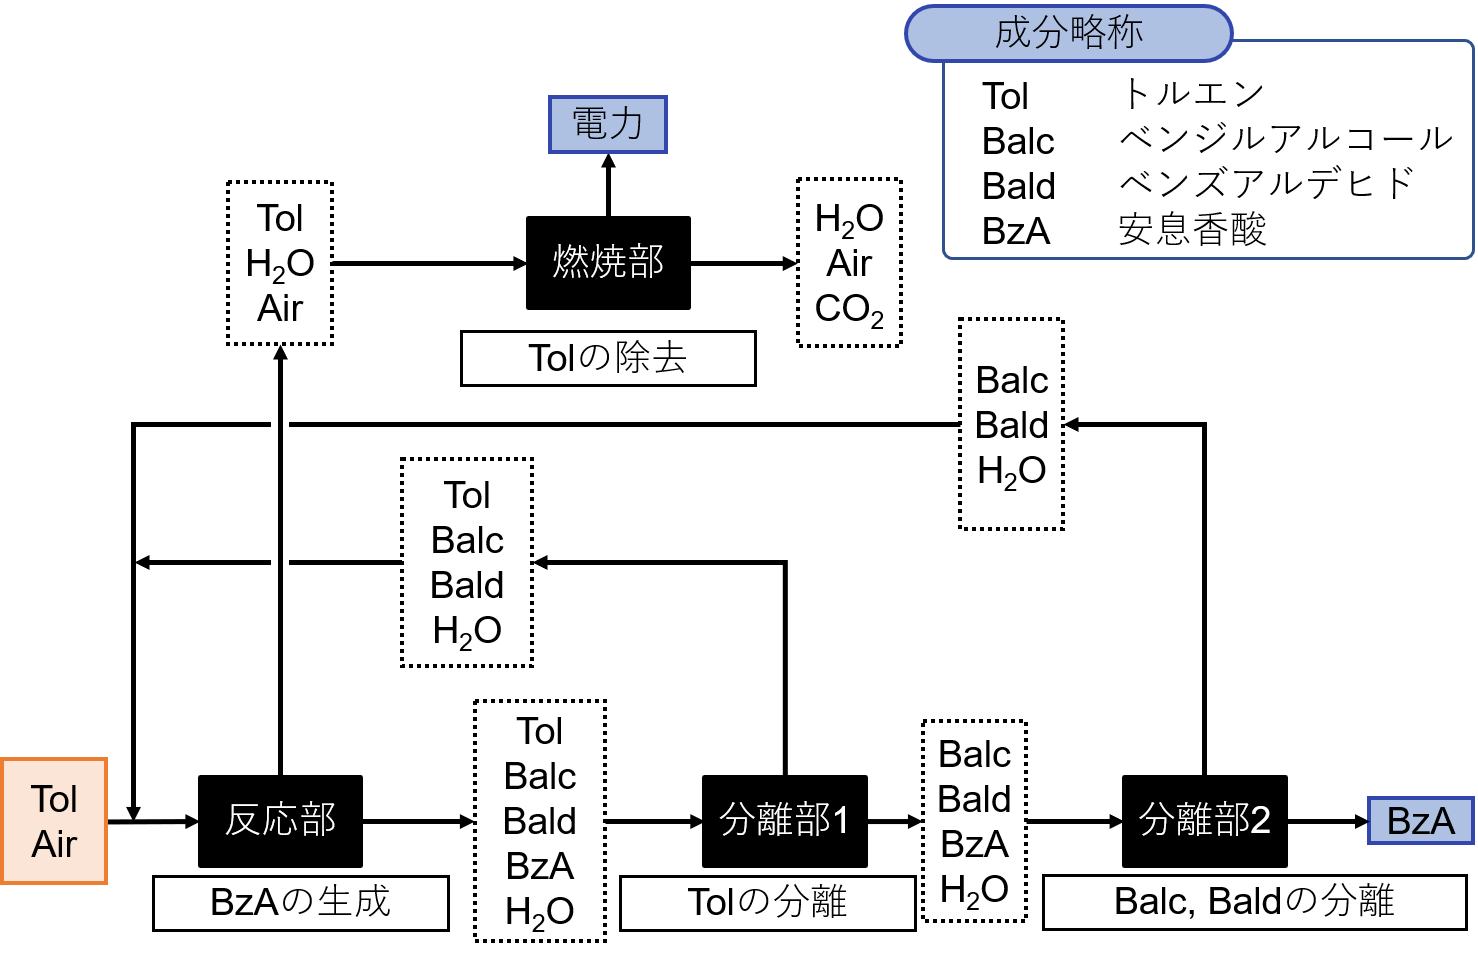
\includegraphics[scale=0.6]{processOutline.png}
  \caption{プロセス全体の概略図}
  \label{プロセス全体の概略図}
\end{figure}

\section{設計条件}
プロセスを設計するにあたり,以下の条件を設定した.
\begin{enumerate}
  \item 生産要求は,99.0\,wt\%以上の安息香酸を年2万トンとする.\\
  \item 工場の稼働時間は,1日24時間,年300日とする.\\
  \item 原料として,純度100\,\%のトルエンおよび,組成を窒素79\,mol\%酸素21\,mol\%とする空気を用いる.
           ただし,両原料は25\,\si{degreeCelsius},1\,\si{\bar}で供給されるものとする.\\
  \item 減価償却期間は8年とする.\\
  \item 圧力損失,熱損失,制御系については考慮しない.\\
  \item HYSISを用いての物性推算はUNIQUAC式によって行う.
\end{enumerate}


\clearpage
\chapter{反応部}
トルエンを空気酸化させ,安息香酸に転化させることを目的とする工程である.
反応部の概略図を図 \ref{反応部設計結果の概略図} に示す.
反応器にフィードされる液は,原料およびリサイクルによって回収された未反応トルエン,ベンジルアルコール,ベンズアルデヒド,水であり,反応器入り口において7\,\si{\bar},170\,\si{\degreeCelsius}に加熱および加圧され,反応器に供給される.また,反応器底部からは空気が1\,\si{\bar},25\,\si{\degreeCelsius}で供給されており,攪拌されながら反応器上方に向かう.反応器内は外部熱煤によって加熱され,7\,\si{\bar},170\,\si{\degreeCelsius}に保たれており,攪拌によって液中に溶けた酸素と未反応物質は触媒酸化反応を起こす.また,気液間物質移動により,液中のトルエンおよび水が盛んに蒸発するが,蒸発したトルエンおよび水を含む空気は反応器からコンデンサーに流入し凝縮される.凝縮したトルエンおよび水はデカンターへ送られ,密度差分離によりトルエンのみを反応器に還流し,水はパージする.また,凝縮しなかったトルエンは,環境安全上の理由からそのまま排出することはできないので,濃度を減少させるために燃焼部へと送られる.反応器からの流出液は次の工程である分離部1へと送られる.
\begin{figure}[htbp]
  \centering
  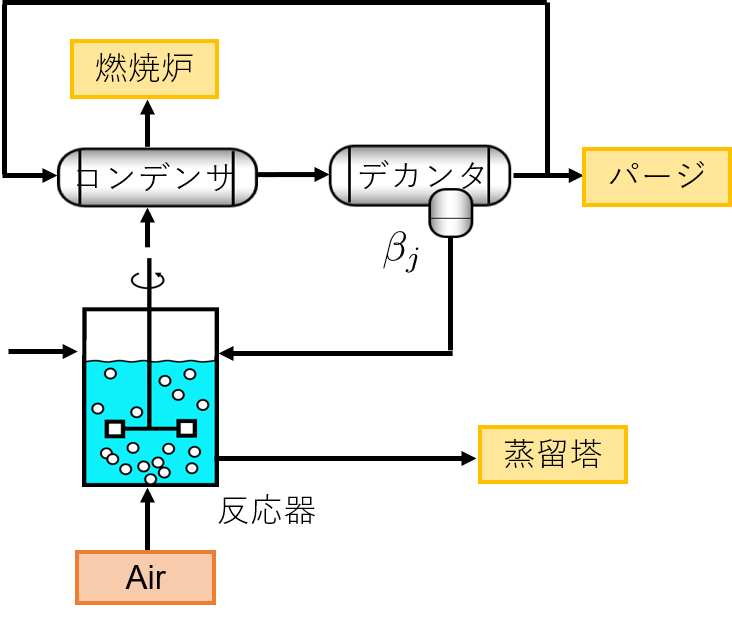
\includegraphics[scale=0.7]{ReactionSection.png}
  \caption{反応部概略図}
  \label{反応部設計結果の概略図}
\end{figure}

\section{反応機構}
今回用いた反応を以下に示す.それぞれの反応速度式および,298\,\si{\kelvin}における反応エンタルピーも示している.トルエンは経路によらず最終的に安息香酸へと転化する.
\begin{center}
\begin{tabular}{lcrlll}
  \ce{Tol} & + & \ce{O2} & \ce{-> Bald + H2O} & $r_1 = k_1 \cdot C_\text{Tol}$ & $\varDelta _\mathrm{r} H_1 = -385.23$ \, \si{\kilo \joule \per \mole} \\
  \ce{Tol} & + & 1/2 \ce{O2} & \ce{-> Balc} & $r_2 = k_2 \cdot C_\text{Tol}$ & $\varDelta _\mathrm{r} H_2 = -167.30$ \, \si{\kilo \joule \per \mole} \\
  \ce{Balc} & + & 1/2 \ce{O2} & \ce{-> Bald + H2O} & $r_4 = k_3 \cdot C_\text{Balc}$ & $\varDelta _\mathrm{r} H_3 = -317.30$ \, \si{\kilo \joule \per \mole} \\
  \ce{Bald} & + & 1/2 \ce{O2} & \ce{-> BzA} & $r_3 = k_4 \cdot C_\text{Bald}$ & $\varDelta _\mathrm{r} H_4 = -298.20$ \, \si{\kilo \joule \per \mole}
\end{tabular}
\end{center}

ただし,トルエンをTol,ベンジルアルコールをBalc,ベンズアルデヒドをBald,安息香酸をBzAと表記している.これらの反応は全て酸化反応であり,触媒には,酸化剤であるモリブデン酸マンガン\ce{MnMoO4}を用いることとした.これらの反応の反応速度定数は,表\ref{反応速度定数}のようである\cite{HOORN2005187}.
\begin{table}[htbp]
  \centering
  \label{反応速度定数}
  \caption{各反応式の反応速度定数}
  \begin{tabular}{ccccc}
    \hline
    & $k_1$ & $k_2$ & $k_3$ & $k_4$ \\
    \hline
    $\ln A_j \, [\si{-}]$ & 17.93 & 20.63 & 15.40 & 19.70 \\
    $E_j \, [\si{\kilo \joule \per \mole}]$ & 69.53 & 81.39 & 56.99 & 71.44 \\
    \hline
  \end{tabular}
\end{table}

また,酸化反応が激しい場合には燃焼反応によって二酸化炭素まで転化するので,反応器における反応率が高い場合には考慮する必要があるが,
今回の設計結果では単通反応率が0.265と低いため,燃焼反応は十分無視できる考えられる.

\section{反応器選定}
流通式の気液反応器の種類には,拡散速度に対して不利な順に,気泡塔,気液攪拌槽,充填塔などがある.
反応器を選定するにあたり,最大反応速度と最大拡散速度の比を表す八田数を概算し,八田数が0.1より小さいなら気泡塔,5より大きければ充填塔,中間域ならば気液攪拌槽を選択することとした\cite{化工便覧}.
今回は気液攪拌槽型反応器を選択した.実際のプロセスでは気泡塔も選択される.

反応器内攪拌には6枚羽根タービン翼を用い,空気流入による冷却作用が大きいため,ジャケットを取り付け,ジャケット内部に熱媒を流している.
また,空気を反応器内に送るスパージャー直径は反応器直径の1/3とした.反応装置はL/D比が2であり,うち半分は液相部のみの体積が占める.\\

八田数の定義式
\begin{equation}
    \gamma = \frac{\text{(最大反応速度)}}{\text{(最大拡散速度)}} = \frac{(C_\mathrm{B} k D_\mathrm{B})^{1/2}}{k_\mathrm{L}}
\end{equation}

\section{設計方程式}
両相の滞留時間の大きさが十分異なると考えられることから,
液相は完全混合状態として,気相は鉛直方向に向かう押し出し流れと仮定できると判断した.
設計時に用いた仮定は以下のようである.
\begin{itemize}
    \item[-] 気相は水平方向に一様な濃度分布を持つ.
    \item[-] 気相側境膜抵抗は無視できる
    \item[-] 液相は完全混合状態である.
    \item[-] 窒素,酸素はヘンリー則に従い,その他の物質はラウール則に従う.
\end{itemize}
以上の仮定および,蒸発油分を還流する機構を含めて,設計方程式\eqref{液相物質収支式},\eqref{気相物質収支式},\eqref{熱収支式}を立式した.
\begin{equation}
    \label{液相物質収支式}
    0 = F^\text{in}_{\text{liq},j} - F^\text{out}_{\text{liq},j} - (1 - \beta_j) k_\mathrm{L} a \int^{V_\text{tot}}_0(C_j - C^\text{sat}_j) \diff V + r_j V_\mathrm{L}
\end{equation}
\begin{equation}
    \label{気相物質収支式}
    \frac{\diff F_{\text{gas},j}}{\diff V} = k_\mathrm{L} a (C_j - C^\text{sat}_j)
\end{equation}
\begin{equation}
    \label{熱収支式}
    \sum_jF_{j,\mathrm{in}}H_{j,\mathrm{in}}-\sum_jF_{j,\text{out}}H_{j,\text{out}} = UA(T_\mathrm{s}-T)
\end{equation}

解析方法としては,まず油分を全還流として近似的に各液相中濃度を決定した.そして,トルエンおよび,酸素,窒素について濃度を仮定した後に,
気相の物質収支式をRunge-kutta法によって計算し,各蒸発量が収支式と一致する濃度を求めた.
また,物質移動容量係数が十分大きいと判断し,最適化中の解析に用いる場合には,気相は迅速に平衡状態へ達すると仮定した.

\section{物質移動容量係数の推算}
物質移動容量係数は,反応装置形状,反応器内部流体の様々な物性,流れの状態に依存する.攪拌槽型反応器に対し,物質移動容量係数の推算に用いた各相関式を記す.

\noindent 液相側物質移動係数の相関式\cite{化工便覧}
\begin{align}
  \text{小気泡の場合 : } &k_\mathrm{L} = 0.31Sc_\mathrm{L}^{-2/3}(g \varDelta \rho \mu_\mathrm{L}/\rho_\mathrm{L}^2)^{1/3} \\
  \text{大気泡の場合 : } &k_\mathrm{L} = 0.42Sc_\mathrm{L}^{-1/2}(g \varDelta \rho \mu_\mathrm{L}/\rho_\mathrm{L}^2)^{1/3}
\end{align}

\noindent 比表面積の相関式\cite{化工便覧}
\begin{equation}
    a = 1.44 \left( \frac{P_\mathrm{V}^{0.4} \rho_\mathrm{L}^{0.2} }{ \sigma^{0.6}} \right) \left( \frac{u_\mathrm{G}}{u_\mathrm{t}} \right)^{0.5} \left( \frac{P_\mathrm{T}}{P_\mathrm{G}} \right) \left( \frac{\rho_\mathrm{G}}{\rho_\mathrm{a}} \right)^{0.16}
\end{equation}

上記の2式を利用するために用いた相関式を以下に記す.

\noindent ガスホールドアップの相関式\cite{化工便覧}
\begin{equation}
    \varepsilon_{{\mathrm G}} = \left( \frac{u_{{\mathrm G}}\varepsilon_{{\mathrm G}}}{u_{{\mathrm t}}} \right) + 0.000216 \times \left( \frac{P_\mathrm{V}^{0.4} \rho_\mathrm{L}^{0.2} }{ \sigma^{0.6}} \right) \left( \frac{u_\mathrm{G}}{u_\mathrm{t}} \right)^{0.5} \left( \frac{P_\mathrm{T}}{P_\mathrm{G}} \right) \left( \frac{\rho_\mathrm{G}}{\rho_\mathrm{a}} \right)^{0.16}
\end{equation}

\noindent 気泡の体積平均径の相関式\cite{化工便覧}
\begin{equation}
    d_\mathrm{vs} = 4.15 \left( \frac{\sigma^{0.6}}{P_\mathrm{V}^{0.4} \rho_\mathrm{L}^{0.2}} \right) \left( \frac{P_\mathrm{G}}{P_\mathrm{T}} \right) \left( \frac{\rho_\mathrm{a}}{\rho_\mathrm{G}} \right) ^{0.16} \varepsilon_\mathrm{G}^{0.5} + 0.0009
\end{equation}

\noindent 気泡の終末速度の相関式\cite{化工便覧}
\begin{equation}
    u_\mathrm{t} = \left( \frac{4\varDelta \rho g d_\mathrm{vs}}{3C_\mathrm{D} \rho_\mathrm{L}} \right)^{0.5}
\end{equation}

さらに,上記の相関式を利用するために用いた物性値の推算式,および変数の定義式などの諸式を以下に記す.

\noindent 抗力係数の相関式\cite{19952357}
\begin{equation}
    C_\mathrm{D} = \max \left[ \frac{24}{Re}(1+0.15Re^{0.687}), \, \frac{8}{3} \frac{Eo}{Eo+4} \right]
\end{equation}
拡散係数の推算\\
wilke-changの式\cite{wilke}
\begin{equation}
    D_{12} = \frac{2.946\times 10^{-11}(\beta M_{\mathrm{r,2}})^{1/2} T} {\mu_2 V_{\mathrm{b},1}^{0.6}}
\end{equation}
Einstin-Stokesの式\cite{実験テキスト}
\begin{equation}
    \frac{D \mu}{T} = \text{const}
\end{equation}

\noindent 界面張力の推算

\noindent 界面張力の温度依存性に関する相関式\cite{化工便覧}
\begin{equation}
    \sigma \propto \{ 1-(T/T_\mathrm{c}) \}^n
\end{equation}

\noindent 気泡レイノルズ数の定義式\cite{19952357}
\begin{equation}
    Re = \frac{\rho_\mathrm{L}u_\mathrm{t} d_\mathrm{vs}}{\mu_\mathrm{L}}
\end{equation}
\noindent エトベス数の定義式\cite{19952357}
\begin{equation}
    Eo = \frac{g \varDelta \rho d_\mathrm{vs}^2}{\sigma}
\end{equation}

また,空気の沸点における分子容を\,29.9\si{\cubic \centi \metre \per \mole}とし\cite{化工便覧},
トルエンの界面張力を$\sigma=0.81 \,\si{\newton \per \metre \squared}$とし\cite{界面張力},
会合度を1とした\cite{TPP}.

以上の諸式を用いて物質移動容量係数を推算した.結果は反応器設計結果で示す.

\section{反応器設計結果}
最終結果における反応器の詳細を表\ref{反応器設計結果の表}に示す.ただし,反応器内温度は,外部熱煤を用いることで,
170\,\si{\degreeCelsius}に保たれているとした.
\begin{table}[htbp]
  \centering
  \caption{反応器設計結果}
  \label{反応器設計結果の表}
  \begin{tabular}{cc}
    \hline
    項目 & 値 \\
    \hline
    反応器内圧力 \, [\si{bar}] & 7.00 \\
    反応器内温度 \, [\si{\degreeCelsius}] & 170 \\
    反応器体積 \, [\si{\cubic \metre}] & 14.6 \\
    気液総体積 \, [\si{\cubic \metre}] & 8.25 \\
    単通販能率 \, [\si{-}] &0.265\\
    ガスホールドアップ \, [\si{-}] & 0.115  \\
    液平均滞留時間 \, [\si{\hour}] & 0.478  \\
    物質移動容量係数 \, [\si{\per \second}] & 0.470  \\
    液相物質移動係数 \, [\si{\metre \per \second}] & 0.00172 \\
    比界面積 \, [\si{\per \metre}] & 273 \\
    反応器空間率 \, [\si{-}] & 0.435 \\
    総攪拌動力 \, [\si{\kilo \watt}] & 8.25 \\
    気泡体積平均径 \, [\si{\milli \metre}] & 2.53 \\
    エトベス数 \, [\si{-}] & 1480 \\
    気泡レイノルズ数 \, [\si{-}] & 1170 \\
    \hline
  \end{tabular}
\end{table}

\section{反応部設計結果}
最適化後の最終結果における反応部の物質収支を図\ref{反応部設計結果の図}中に示す.最適化方法については最適化の章で述べる.
\begin{figure}[htbp]
  \centering
  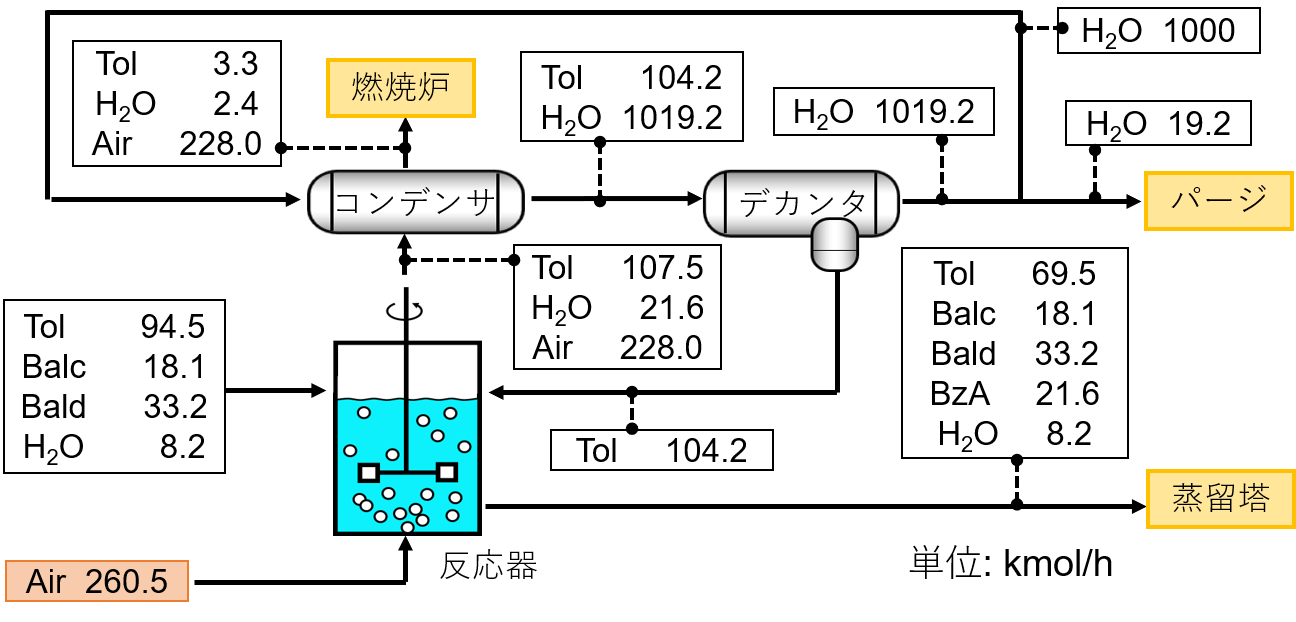
\includegraphics[scale=0.7]{ReactionSectionConclusion.png}
  \caption{反応部設計結果}
  \label{反応部設計結果の図}
\end{figure}


\clearpage
\chapter{分離部1}
反応器からの流出液のうち,主に未反応トルエンを分離することを目的とする工程である.トルエンおよび低沸点成分である水は蒸留によってほぼ全量が回収され,回収しきれなかったベンジルアルコールやベンズアルデヒド,安息香酸およびモリブデン酸マンガン触媒は分離工程2へと送られる.
\section{蒸留塔設計}
未反応トルエンのうち99\,\%以上を回収することを目的とした.
設計条件として,蒸留塔段数を10段,蒸留塔供給段は6段,還流比を1.0とした.

蒸留塔圧力を変更し,全体の利益を最大とする点について探索を行った.
反応器流出液圧力が7\,\si{\bar}であるため,最適な圧力であることが予想される.
蒸留塔の圧力を変化させ,人件費を除く全体の利益を評価関数としてプロットした
図\ref{蒸留塔圧力最適化}から,確かに7\,\si{\bar}で全体の利益が最大化されることを確認した.
\begin{figure}[htbp]
  \centering
  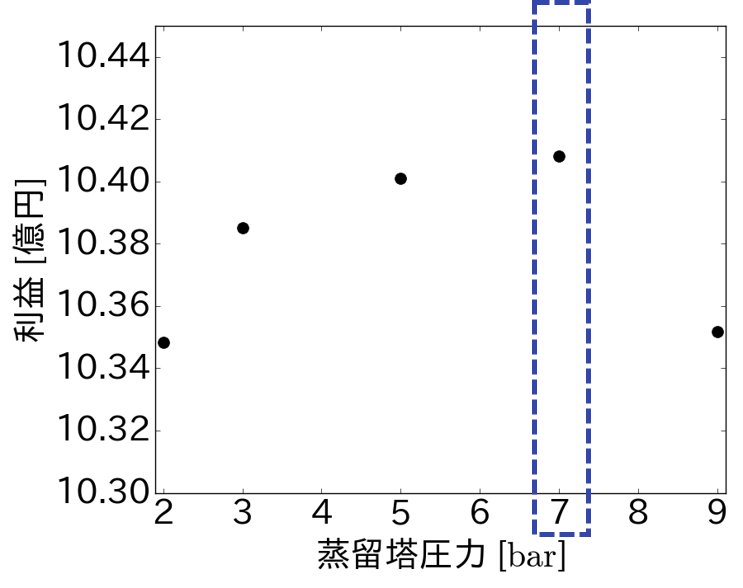
\includegraphics[scale=0.7]{DistillationPressue.png}
  \caption{蒸留塔圧力最適化}
  \label{蒸留塔圧力最適化}
\end{figure}

設計結果を表\ref{蒸留塔設計結果}に記す.
\begin{table}[htbp]
  \label{蒸留塔設計結果}
  \caption{蒸留塔設計結果}
  \centering
  \begin{tabular}{cc}
      \hline
      項目 & 値 \\
      \hline
      塔径 \, [\si{\metre}] & 1.0 \\
      塔高 \, [\si{\metre}] & 6.1 \\
      塔内圧力 \, [\si{\bar}] &7 \\
      コンデンサ内温度 \, [\si{\degreeCelsius}] & 232 \\
      リボイラー内温度 \, [\si{\degreeCelsius}] & 316 \\
      \hline
  \end{tabular}
\end{table}

\section{分離部1設計結果}
最適化後の最終結果における分離部1の流量関係を図\ref{分離部1設計結果の図}中に示す.
\begin{figure}[htbp]
  \centering
  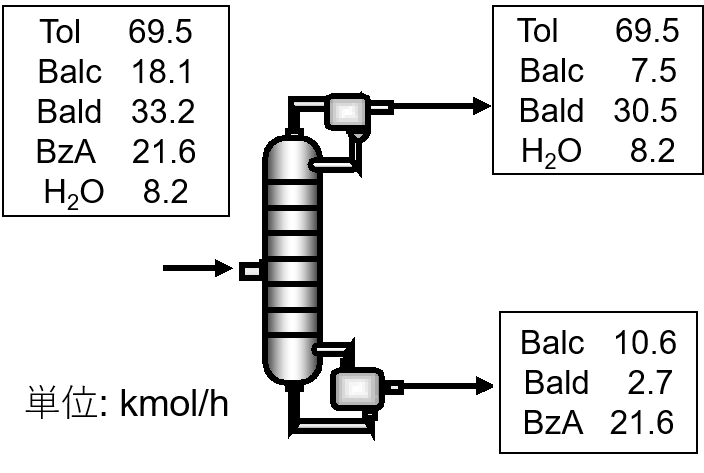
\includegraphics[scale=0.7]{Separation1Conclusion.png}
  \caption{分離部1設計結果}
  \label{分離部1設計結果の図}
\end{figure}


\clearpage
\chapter{分離部2}
他成分を分離し,安息香酸の製品結晶を得る工程である.蒸留塔の流出液に含まれるベンジルアルコール,ベンズアルデヒド,安息香酸,モリブデン酸マンガン触媒を抽出塔に送り,晶析後の安息香酸水溶液をリサイクルして同時に抽出塔に入れ,安息香酸とその他の成分を分離する.安息香酸飽和水溶液は晶析器に運ばれ,製品結晶を取り出す.その他の成分については回収し,反応器へと循環させる.

\section{晶析器選定}
結晶,溶液をともに連続的に流通させることができる連続式の晶析装置を選択した.
溶解度の温度依存性が大きいことと,目的とする結晶生産量が大きいことから,連続式攪拌槽型反応装置を選定した.
結晶は針状であり,一般的な球形の結晶よりも装置内に詰まる恐れがある\cite{化工便覧}.よって製品結晶のみが固体状で装置内を占めると想定して,空間率が0.9以上となるように十分な装置容積をとる必要があるため,晶析装置内液相部の2倍の装置容積を用意するものとして設計した.
L/D比は2とした.


\noindent 溶解度の温度依存性の相関式
\begin{equation}
    C^*=2.03\times 10^{-5}T^4 +2.03^{-5}\times T^4 + 2.97\times 10^{-4}T^3 + 4.70\times 10^{-2}T^2 + 1.43T + 24.71
\end{equation}
ただし,温度$T \, [\si{\degreeCelsius}]$,溶解度$C^* \, [\si{\gram \per \kilo \solventgram}]$
\begin{figure}[htbp]
  \centering
  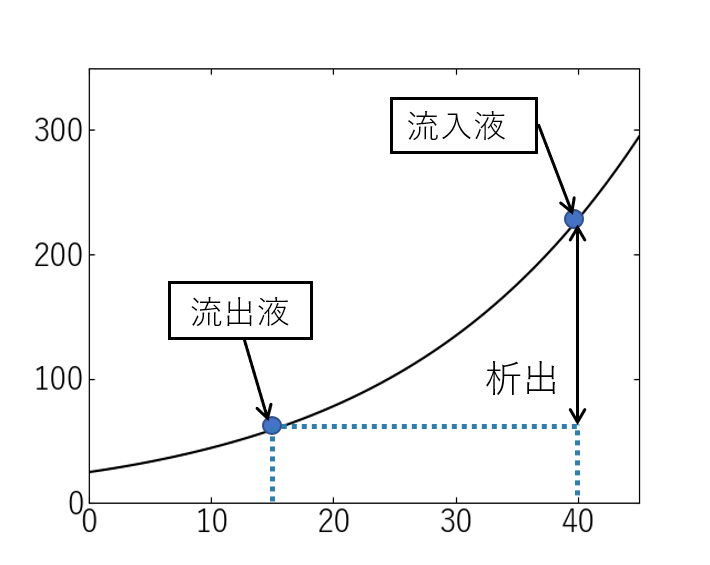
\includegraphics[scale=0.7]{BzAsolvent.png}
  \caption{溶解度の温度依存性}
  \label{溶解度の温度依存性}
\end{figure}

\section{設計方程式}
以下の仮定を用いた.
\begin{itemize}
    \setlength{\parskip}{0pt}
    \setlength{\itemsep}{2pt}
    \item[-] 結晶表面拡散は迅速に行われる.
    \item[-] 晶析器内は完全混合状態である.
    \item[-] 二次核発生の影響は無視する.
\end{itemize}

\cite{晶析}により,以下の実験式および理論式を用いて設計を行った.\\
一次核発生速度
\begin{equation}
    B^0 = k_\mathrm{b} M_\mathrm{T}^j \varDelta C^b
\end{equation}
結晶成長速度
\begin{equation}
    G = k_\mathrm{g} \varDelta C^g
\end{equation}
結晶成長速度定数
\begin{equation}
    k_\mathrm{g} = k_\mathrm{g0} \exp \left( -\frac{E_\mathrm{g}}{RT} \right)
\end{equation}
個数収支式
\begin{equation}
    n=n^0 \exp \left( -\frac{L}{G\tau} \right)
\end{equation}
懸濁密度
\begin{equation}
    M_\mathrm{T} = c_0-c = 6k_\mathrm{v} \rho_\mathrm{c} n^0 (G\tau)^4
\end{equation}
各パラメータは以下の通りである.
\begin{align*}
    &k_\mathrm{g0} = 1.06\times10^7 \, \si{(\micro \meter)(\gram / \solventgram)^{\textit{-g}}} \\
    &B^{\mathrm{0}} = 40.05 \, \si{\kilo \joule \per \mole} \\
    &k_\mathrm{b} = 9.16 \times 10^{12} \, \si{(\# / \cubic \meter \second) (\gram / \milli \liter)^{\textit{-j}} (\gram / \solventgram)^{\textit{-b}}} \\
    &g = 0.44 \\
    &j = 1.78 \\
    &b = 1.2 \\
    &k_\mathrm{v} = 0.1 \\
    &\rho_\mathrm{c} = 1.32 \, \si{\gram \per \centi \metre \cubed}
\end{align*}

\section{晶析器設計結果}
最適化の結果によって得られた晶析器の設計結果を表\ref{晶析器設計結果}に記す.
\begin{table}[htbp]
  \centering
  \caption{晶析器設計結果}
  \label{晶析器設計結果}
  \begin{tabular}{cc}
    \hline
    項目 & 値 \\
    \hline
    晶析器体積 \, [\si{\cubic \metre}] &7.16 \\
    晶析器液体積 \, [\si{\cubic \metre}] &3.58 \\
    晶析器フィード液温 \, [\si{\degreeCelsius}] & 40.0 \\
    晶析器内温度 \, [\si{\degreeCelsius}] &13.3 \\
    晶析器内圧力 \, [\si{bar}] &1.00 \\
    滞留時間 \, [\si{min}] &9.71 \\
    単通結晶収率 \, [\si{-}] &0.690 \\
    結晶化可能量基準収率 \, [\si{-}] &0.902 \\
    結晶の体積平均径 \, [\si{\micro \metre}] &3.41 \\
    \hline
  \end{tabular}
\end{table}

\section{抽出塔設計}
十分に塔内へ液を滞留させることによって安息香酸を水中に飽和させることを目的とした.
十分なデータを得られなかったため,2時間の装置内滞留によって安息香酸がトルエン溶媒中に飽和し,
その他ベンジルアルコール,ベンズアルデヒドの溶解度については無視できると仮定した.

\section{分離部2設計結果}
分離部2のみの流量関係を簡易的に図\ref{分離部2設計結果}中に示す.
蒸留塔から送られてきた油液は冷却され,抽出塔内に供給される.晶析器で用いた安息香酸水溶液を加熱し,溶解度を上昇させて抽出塔内に供給する.
抽出塔内では安息香酸が水中に溶解し,ベンジルアルコール,ベンズアルデヒドおよび触媒は溶解せずに回収され,反応部へ送られる.安息香酸水溶液を晶析器に供給し,製品結晶を得ている.

\begin{figure}[htbp]
  \centering
  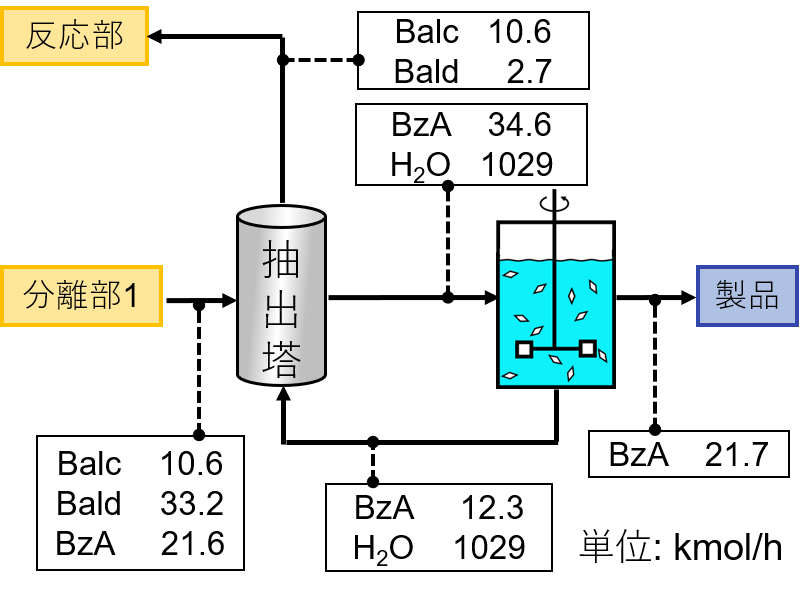
\includegraphics[scale=0.7]{Separion2Conclusion.png}
  \caption{分離部2設計結果}
  \label{分離部2設計結果}
\end{figure}


\clearpage
\chapter{燃焼部}
トルエンは人体に有害な物質であり,吸引によって神経系などに深刻な被害を与えることもある.
排出指針値としてトルエンを扱う作業環境において50\,ppmその他の場所については0.7\,ppmと定められている\cite{トルエン排出基準}.この基準を満たすため,反応部のコンデンサーで凝縮しなかったトルエンを燃焼させることでその濃度を減じる.
燃焼炉内ではトルエンが完全燃焼し,二酸化炭素および水へ転化すると仮定し,量論的に燃焼に必要な量と等量の酸素を供給して燃焼炉へと送るものとした.
燃焼熱は熱媒の作成に使用され,足りない分は燃料を投入して賄っているものと考えた.

\clearpage
\chapter{最適化}
\section{方法}
最適化を行うにあたり,最適化変数として以下の3つを選択した.
\begin{itemize}
  \item 反応器体積
  \item 晶析器体積
  \item 晶析器温度
\end{itemize}

これらの変数を選択した理由を述べる.反応器体積が大きいとき,反応器の装置コストは大きくなる.一方で,反応器出口から排出される未反応トルエンの量が減るため,蒸留塔のリボイラーで必要な熱量が減少し,熱煤のコストは減少する.反応器体積が小さいときは,反応器の装置コストは小さくなるが,熱煤のコストは大きくなる.晶析器体積が大きいとき,晶析器の装置コストは大きくなる.しかし,晶析する安息香酸の量が増えるため,リサイクルに回る安息香酸の量が少なくなり,それを保持するための純水の量が減少し,純水の費用は抑えられる.晶析器の体積が小さいときは,逆になる.晶析器温度が低い時,必要な外部冷媒の温度が低くなるため,冷媒の単価は高くなる.しかし,晶析する安息香酸の量が大きくなるため,リサイクルに回る安息香酸の量が小さくなり,必要な純水の量が減るため,純水を冷やすために用いている冷媒の量は小さく抑えられる.晶析器温度が高いときは,冷媒の単価は安くなるが,冷媒の必要量が大きくなる.このように,最適化変数に選択した変数は,その大小によって,なんらかのトレードオフの関係を生じる.そのため,これらの変数の値を変化させることで,利益が最大となる最適点を探索することが可能であると考えた.

次に,最適化の具体的な手法について述べる.プロセスを最適化するにあたり,3つの最適化変数変数全てを同時に最適化することを考えた.そこで,反応器体積は,$13.5 \sim 16.0 \, \si{\cubic \metre}$の範囲で6点,晶析器体積は,$6 \sim 12 \, \si{\cubic \metre}$の範囲で13点,晶析器温度は,$5.0 \sim 20.0 \, \si{\degreeCelsius}$の範囲で16点,計1248点のデータを取った.そして,それぞれのデータについてフィッティングを行った後に,それぞれの範囲を100当分し,データの個数を$100 \times 100 \times 100$点に増やした.それらのデータを用いて,横軸に晶析器温度,縦軸に晶析器体積を設定し,反応器体積の値を逐次的に変化させることで,100枚のヒートマップを作成した.ヒートマップが表す値は,
\begin{equation}
  \text{P.I.} = \text{(売上)} - \text{(原料コスト)} - \text{(装置コスト)} -\text{(用役コスト)}
\end{equation}
で表される評価関数の値とした.また,各ヒートマップ上で,評価関数の値が最大となる点をプロットした.さらに,そのプロットがどのように変化するかを見るために,横軸に反応器体積,縦軸に評価関数の値を取り,折れ線グラフを作成した.

\section{最適化結果}
評価関数の値が最大となった点での,ヒートマップおよび,評価関数の最大値の変化を表したグラフは図\ref{最適化結果}のようになった.また,作成したgifはgithubにアップしているので,興味のある方はご覧ください(\url{https://github.com/miyamo-sou/processdesign}).最適点での反応器体積は14.69\, \si{\cubic \metre},晶析器体積は7.16\, \si{\cubic \metre},晶析器温度は13.3\, \si{\degreeCelsius}となった.また,その時の評価関数の値は10.35億円となった.
\begin{figure}[htbp]
  \centering
  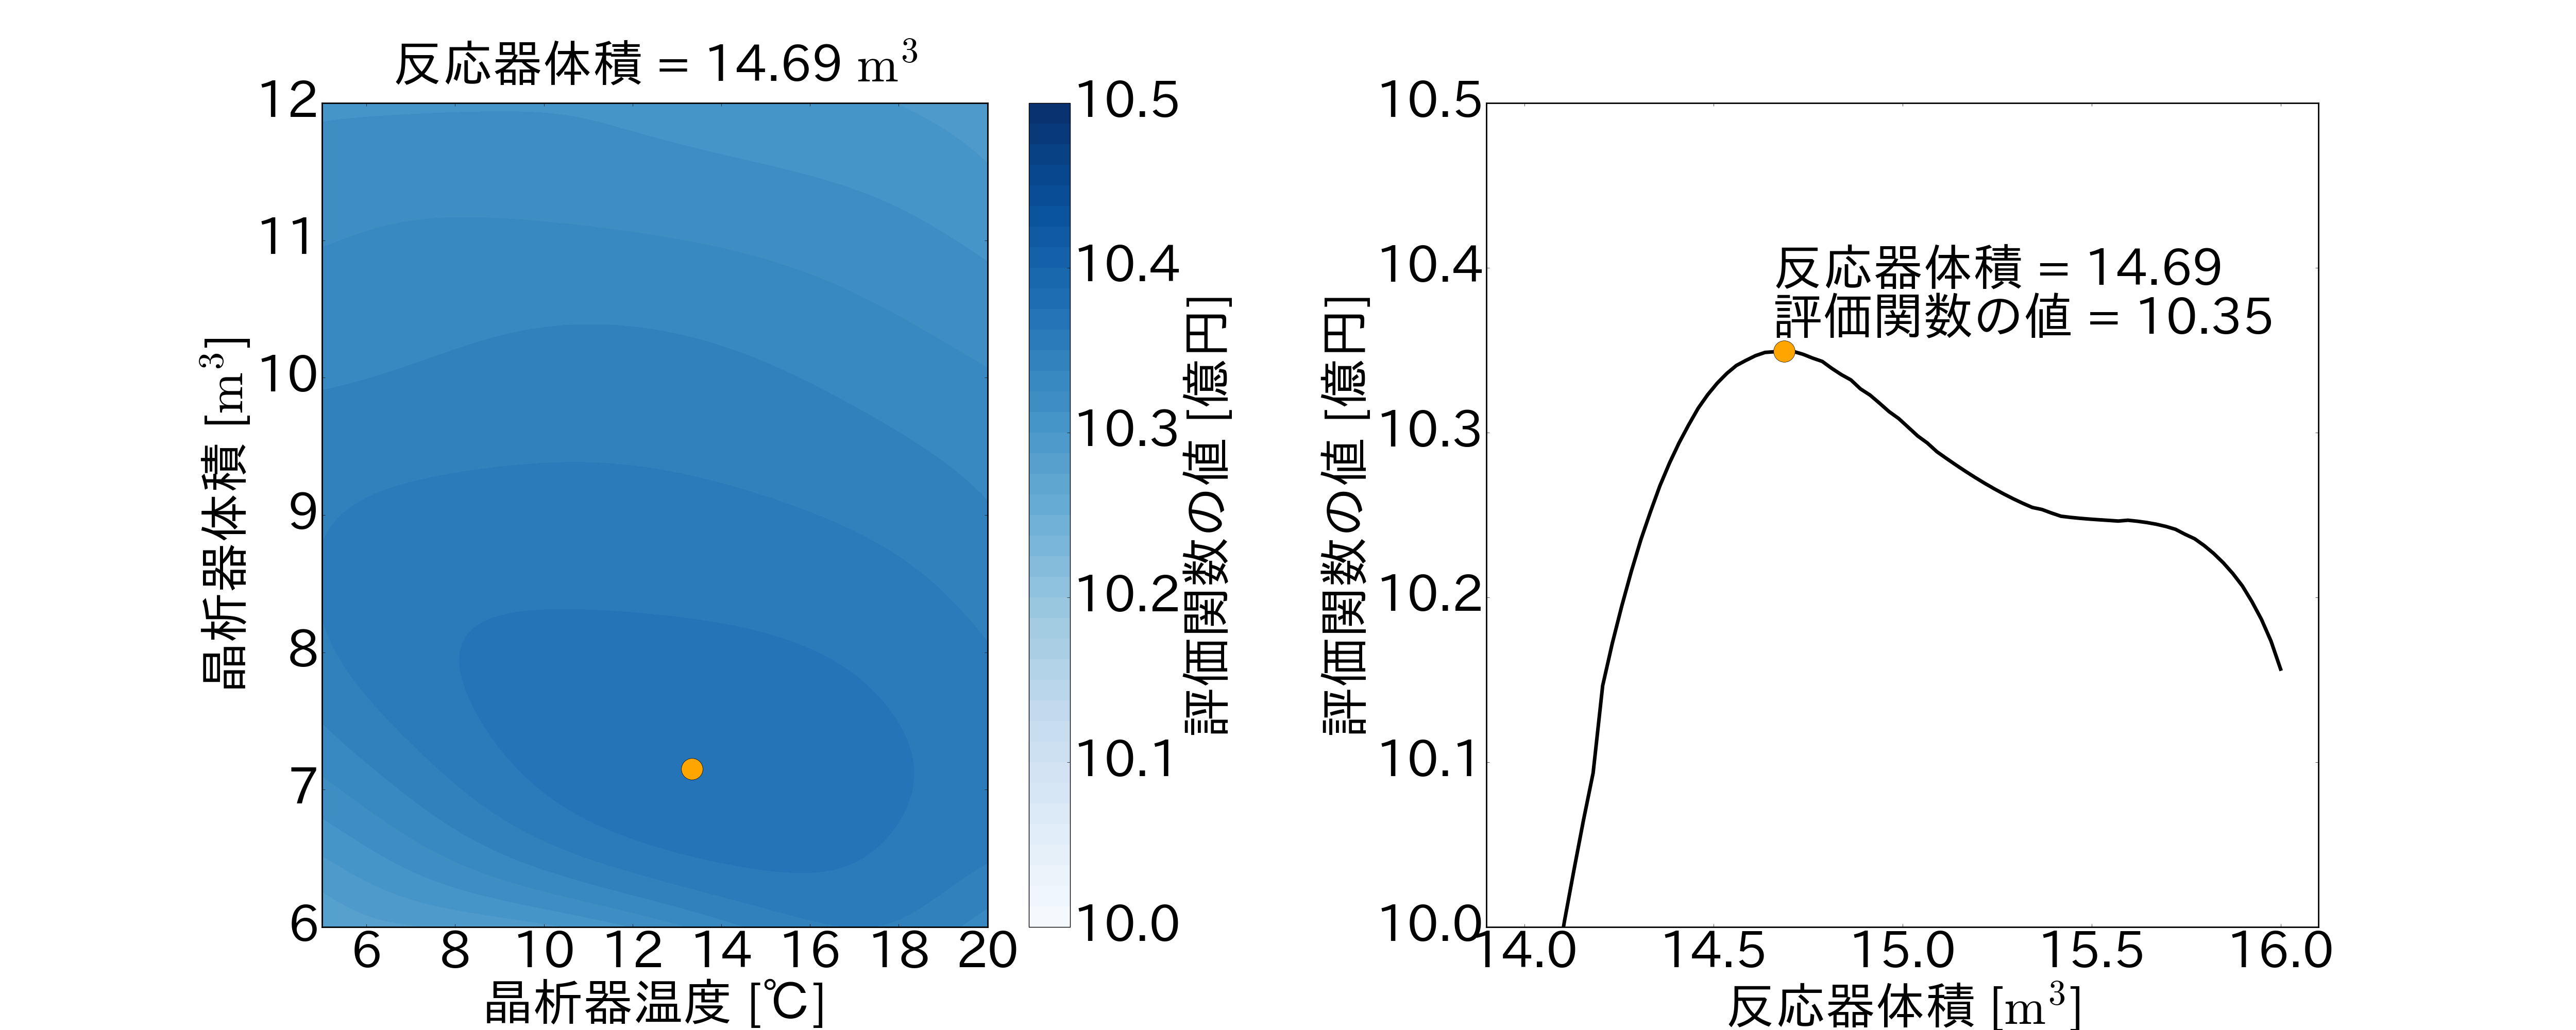
\includegraphics[scale=0.1]{snapshot.png}
  \caption{評価関数の値が最大となる点でのヒートマップと最適点の推移}
  \label{最適化結果}
\end{figure}

このよに,評価関数は大きなピークが存在する形になっていることが分かる.これは,最適化方法のセクションでも述べたが,反応器体積,晶析器体積,晶析器温度を変化させると,装置費と用役費がトレードオフの関係となって,コストが変化する.そのため,このようにピークが生じたと考えられる.


\clearpage
\chapter{物質収支 $\cdot$ 熱収支}
全体のフロー図は図\ref{フロー図}のようになった.
\begin{figure}[htbp]
  \centering
  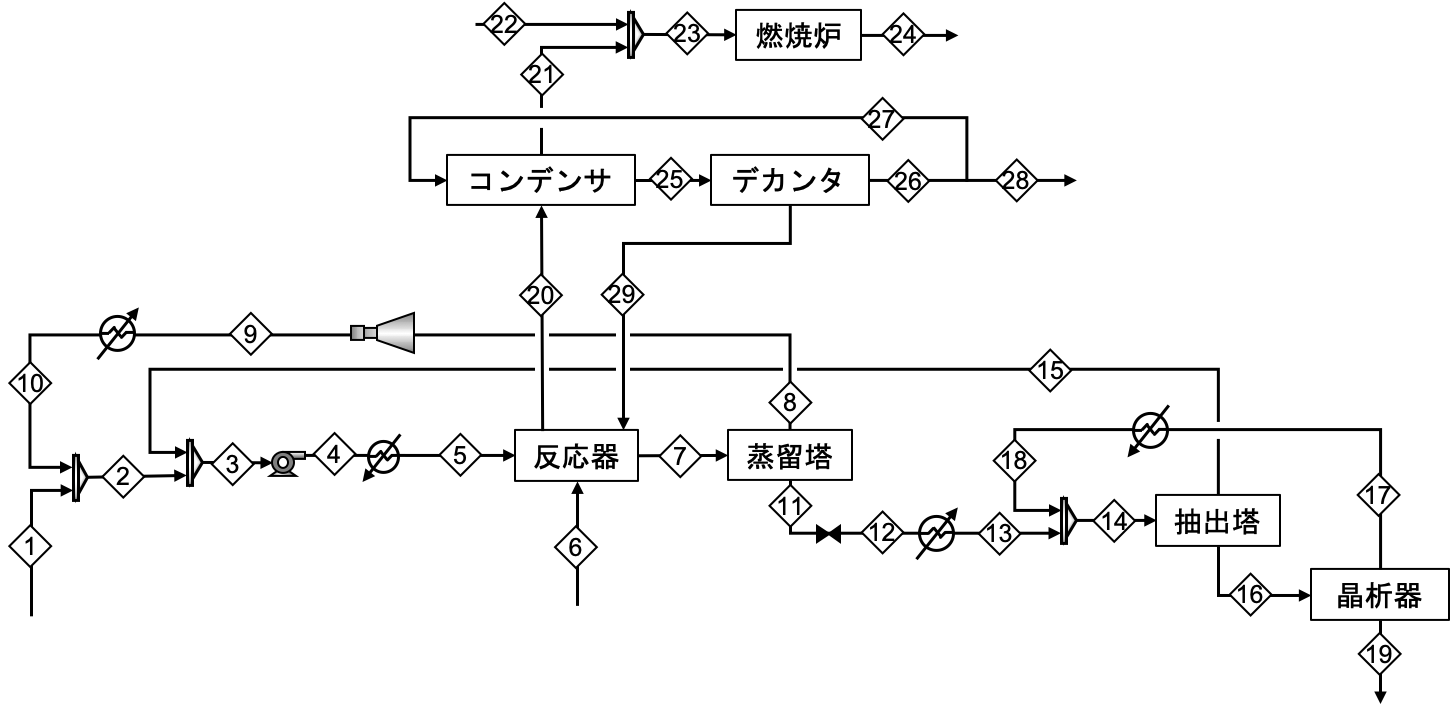
\includegraphics[scale=0.6]{mat_flow.png}
  \caption{フロー図}
  \label{フロー図}
\end{figure}

また,フロー図に記載されているフローの組成および温度,圧力は表\ref{流量関係1},\ref{流量関係2},\ref{流量関係3}のようになった.
\begin{table}[htbp]
  \centering
  \caption{流量関係}
  \label{流量関係1}
  \begin{tabular}{ccccccccccccccc}
    \hline
    [\si{\kilo \mole \per \hour}] & 1 & 2 & 3 & 4 & 5 & 6 & 7 & 8 & 9 & 10 \\
    \hline
    トルエン & 25 & 94.5 & 94.5 & 94.5 & 94.5 & 0 & 69.5 & 69.5 & 69.5 & 69.5 \\
    ベンジルアルコール & 0 & 7.5 & 18.1 & 18.1 & 18.1 & 0 & 18.1 & 7.5 & 7.5 & 7.5 \\
    ベンズアルデヒド & 0 & 30.5 & 33.2 & 33.2 & 33.2 & 0 & 33.2 & 30.5 & 30.5 & 30.5 \\
    安息香酸 & 0 & 0 & 0 & 0 & 0 & 0 & 21.6 & 0 & 0 & 0 \\
    水 & 0 & 8.2 & 8.2 & 8.2 & 8.2 & 0 & 8.2 & 8.2 & 8.2 & 8.2 \\
    空気 & 0 & 0 & 0 & 0 & 0 & 260.5 & 0 & 0 & 0 & 0 \\
    二酸化炭素 & 0 & 0 & 0 & 0 & 0 & 0 & 0 & 0 & 0 & 0 \\
    \hline
    合計 & 25 & 140.7 & 154 & 154 & 154 & 260.5 & 150.6 & 115.7 & 115.7 & 115.7 \\
    \hline
    温度 \, [\si{\degreeCelsius}] & 25 & 79.9 & 75.56 & 76.04 & 170 & 25 & 170 & 231.5 & 194.8 & 90.88 \\
    圧力 \, [\si{\bar}] & 1 & 1 & 1 & 7 & 7 & 1 & 7 & 7 & 1 & 1 \\
    \hline
  \end{tabular}
\end{table}

\begin{table}[htbp]
  \centering
  \caption{流量関係}
  \label{流量関係2}
  \begin{tabular}{ccccccccccccccc}
    \hline
    [\si{\kilo \mole \per \hour}] & 11 & 12 & 13 & 14 & 15 & 16 & 17 & 18 & 19 & 20 \\
    \hline
    トルエン & 0 & 0 & 0 & 0 & 0 & 0 & 0 & 0 & 0 & 107.5 \\
    ベンジルアルコール & 10.6 & 10.6 & 10.6 & 10.6 & 10.6 & 0 & 0 & 0 & 0 & 0 \\
    ベンズアルデヒド & 2.7 & 2.7 & 2.7 & 2.7 & 2.7 & 0 & 0 & 0 & 0 & 0 \\
    安息香酸 & 21.6 & 21.6 & 21.6 & 34.6 & 0 & 34.6 & 13 & 13 & 21.6 & 0 \\
    水 & 0 & 0 & 0 & 1029 & 0 & 1029 & 1029 & 1029 & 0 & 21.6 \\
    空気 & 0 & 0 & 0 & 0 & 0 & 0 & 0 & 0 & 0 & 228 \\
    二酸化炭素 & 0 & 0 & 0 & 0 & 0 & 0 & 0 & 0 & 0 & 0 \\
    \hline
    合計 & 34.9 & 34.9 & 34.9 & 1076.9 & 13.3 & 1063.6 & 1042 & 1042 & 21.6 & 357.1 \\
    \hline
    温度 \, [\si{\degreeCelsius}] & 315.6 & 230.9 & 25 & 25 & 40 & 40 & 13.3 & 40 & 13.3 & 25 \\
    圧力 \, [\si{\bar}] & 7 & 1 & 1 & 1 & 1 & 1 & 1 & 1 & 1 & 1 \\
    \hline
  \end{tabular}
\end{table}

\begin{table}[htbp]
  \caption{流量関係}
  \label{流量関係3}
  \centering
  \begin{tabular}{ccccccccccccccc}
    \hline
    [\si{\kilo \mole \per \hour}] & 21 & 22 & 23 & 24 & 25 & 26 & 27 & 28 &  &  \\
    \hline
    トルエン & 3.4 & 0 & 3.4 & 0 & 104.1 & 0 & 0 & 0 &  &  \\
    ベンジルアルコール & 0 & 0 & 0 & 0 & 0 & 0 & 0 & 0 &  &  \\
    ベンズアルデヒド & 0 & 0 & 0 & 0 & 0 & 0 & 0 & 0 &  &  \\
    安息香酸 & 0 & 0 & 0 & 0 & 0 & 0 & 0 & 0 &  &  \\
    水 & 2.4 & 0 & 2.4 & 15.8 & 0 & 0 & 0 & 0 &  &  \\
    空気 & 228 & 39.4 & 267.4 & 237.8 & 1019.2 & 1019.2 & 1000 & 19.2 &  &  \\
    二酸化炭素 & 0 & 0 & 0 & 23.4 & 0 & 0 & 0 & 0 &  &  \\
    \hline
    合計 & 233.8 & 39.4 & 273.2 & 277 & 1123.3 & 1019.2 & 1000 & 19.2 &  &  \\
    \hline
    温度 \, [\si{\degreeCelsius}] & 25 & 25 & 25 & 25 & 25 & 25 & 25 & 25 &  &  \\
    圧力 \, [\si{\bar}] & 1 & 1 & 1 & 1 & 1 & 1 & 1 & 1 &  &  \\
    \hline
  \end{tabular}
\end{table}

\clearpage
フロー全体の与熱流体および,受熱流体は図\ref{与熱流体と受熱流体}のようになった.図中の流体の熱量関係は表\ref{与熱流体}および,\ref{受熱流体}のようになった.
\begin{figure}[htbp]
  \centering
  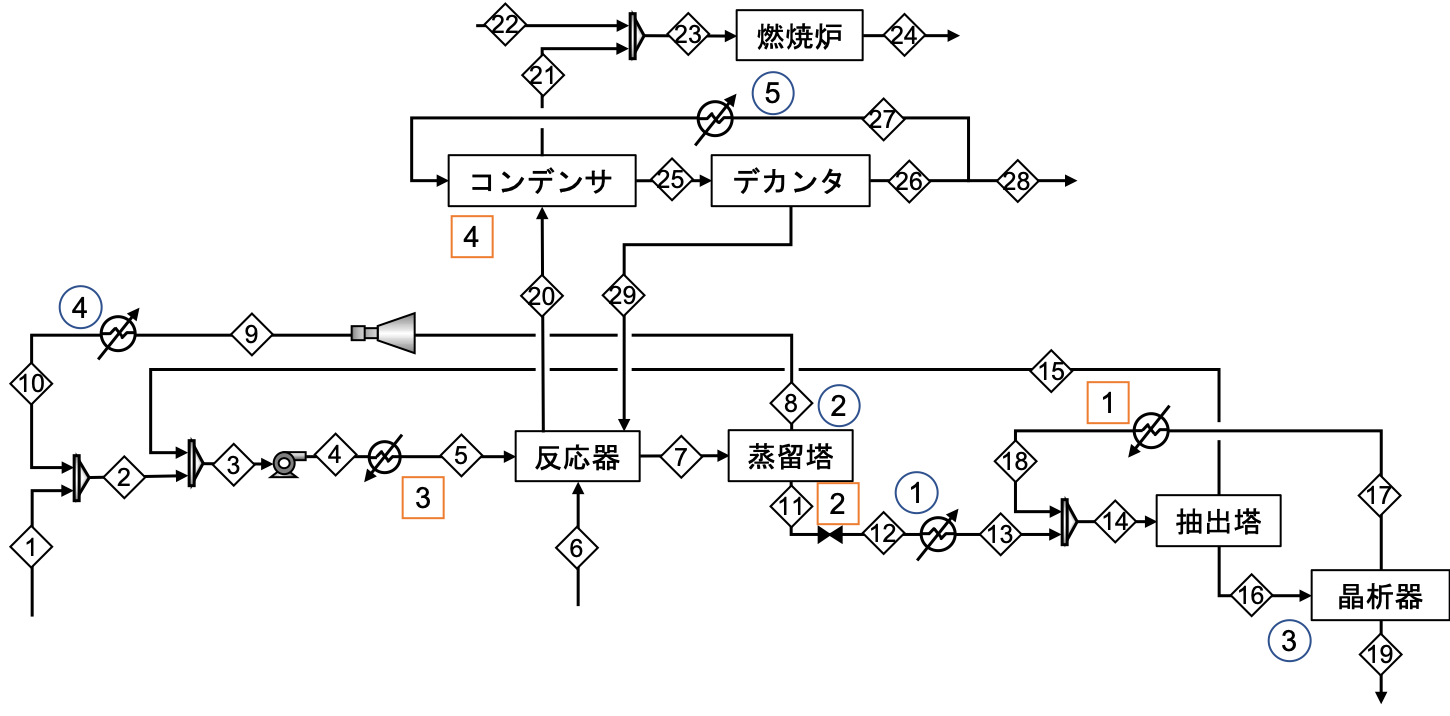
\includegraphics[scale=0.6]{heat_flow.png}
  \caption{与熱流体と受熱流体}
  \label{与熱流体と受熱流体}
\end{figure}

\begin{table}[htbp]
  \centering
  \caption{与熱流体}
  \label{与熱流体}
  \begin{tabular}{lccc}
    \hline
    与熱流体 & 変化前温度 \, [\si{\degreeCelsius}] & 変化後温度 \, [\si{\degreeCelsius}] & 与熱量 \, [\si{\mega \joule \per \hour}] \\
    \hline
    \textcircled{\scriptsize 1} 蒸留塔留出液 & 194.8 & 90.9 & 6338.4 \\
    \textcircled{\scriptsize 2} 蒸留塔コンデンサー & 248.3 & 231.5 & 5111.8 \\
    \textcircled{\scriptsize 3} 晶析器流入流体 & 40.0 & 13.3 & 2252.7 \\
    \textcircled{\scriptsize 4} 蒸留塔缶出液 & 230.9 & 25 & 2436.7 \\
    \textcircled{\scriptsize 5} デカンタ流出純水 & 40.0 & 25 & 1130.6 \\
    \hline
  \end{tabular}
\end{table}

\begin{table}[htbp]
  \centering
  \caption{受熱流体}
  \label{受熱流体}
  \begin{tabular}{lccc}
    \hline
    受熱流体 & 変化前温度 \, [\si{\degreeCelsius}] & 変化後温度 \, [\si{\degreeCelsius}] & 受熱量 \, [\si{\mega \joule \per \hour}] \\
    \hline
    \fbox{\scriptsize 1} 晶析器リサイクル & 13.3 & 40.0 & 2149.3 \\
    \fbox{\scriptsize 2} 蒸留塔リボイラー & 304.0 & 315.6 & 11735.8 \\
    \fbox{\scriptsize 3} 反応器入り口流体 & 76.0 & 170.0 & 2922.4 \\
    \fbox{\scriptsize 4} デカンタ流入純水 & 25.0 & 40.0 & 1130.6 \\
    \hline
  \end{tabular}
\end{table}


\clearpage
\chapter{ヒートインテグレーション}
流体同士の熱交換を行い,外部流体の利用量を削減することを目的としてヒートインテグレーションを行った.
本プロセスにおいては熱交換器は多管型熱交換器として,向流で熱交換を行った.
熱交換面積を求めるため,以下の式を用いた.
\begin{equation}
    Q=UA(\varDelta T)_\mathrm{lm}
\end{equation}
ただし$(\varDelta T)_\mathrm{lm}$は温度差の対数平均であり,熱交換によって与熱流体の温度が$T_\mathrm{h1}$から$T_\mathrm{h2}$に変化し,受熱流体の温度が$T_\mathrm{c2}$から$T_\mathrm{c1}$に変化するとき,
\begin{equation}
    (\varDelta T)_\mathrm{lm} = \frac{(T_\mathrm{h1} - T_\mathrm{c1}) - (T_\mathrm{h2} - T_\mathrm{c2})}{\ln\{(T_\mathrm{h1} - T_\mathrm{c1}) / (T_\mathrm{h2} - T_\mathrm{c2})\}}
\end{equation}
と表される.総括熱伝達係数として,両熱交換流体の相状態にのみ依存するとして表\ref{総括熱伝達係数}の値を用いた.
\begin{table}[htbp]
  \centering
  \caption{総括熱伝達係数}
  \label{総括熱伝達係数}
  \begin{tabular}{ccc}
    \hline
    流体1 & 流体2 & 総括伝熱係数[\si{\watt \per \metre \per \second}] \\
    \hline
    ガス & ガス &150 \\
    ガス & 液 &200 \\
    ガス & ガス(凝縮) & 500 \\
    ガス & 液(蒸発) & 500 \\
    液 & 液 & 300 \\
    液 & ガス(凝縮) & 1000 \\
    液 & 液(蒸発) & 1000 \\
    ガス(凝縮) & 液(蒸発) &1500 \\
    \hline
  \end{tabular}
\end{table}

以下に,用いた外部熱媒の温度と熱量を表\ref{用いた外部熱煤}に示す.
\begin{table}
  \centering
  \caption{用いた外部熱煤}
  \label{用いた外部熱煤}
  \begin{tabular}{ccc}
    \hline
    熱煤 & 温度 [\si{\degreeCelsius}] & 交換熱量 [\si{\kilo \joule \per \hour}] \\
    \hline
    熱煤1 & 330.0 & 11735.8 \\
    熱煤2 & 55.0 & 1085.7 \\
    熱煤3 & 2.3 & 1761.1 \\
    \hline
  \end{tabular}
\end{table}

図\ref{TQ線図}に最終的な設計結果におけるTQ線図を示す.
\begin{figure}[htbp]
  \centering
  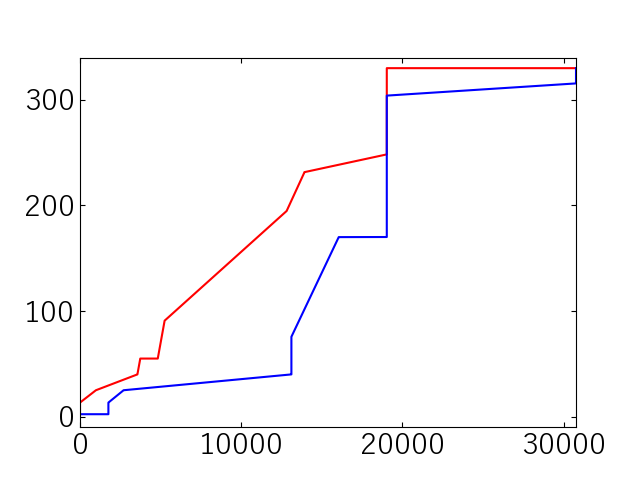
\includegraphics[scale=0.7]{TQ.png}
  \caption{TQ線図}
  \label{TQ線図}
\end{figure}

ヒートインテグレーションを行うことで,必要な外部熱煤の費用は3.6億円から1.2億円にまで削減することができた.

\clearpage
\chapter{経済評価}
減価償却を8年とした場合の経済評価は表\ref{経済評価}のようになった.なお,各装置費の推算式は,Appendix Aに示した通りである.
また,トルエンは500\,\$/\si{\tonne},安息香酸は1013\,\$/\si{\tonne}とした.
\begin{table}[htbp]
    \centering
    \caption{経済評価 [億円/年]}
    \label{経済評価}
    \begin{tabular}{c|c|cc|c}
      \hline
      収入 & 製品 & 安息香酸 & 23.7 & 23.7 \\
      \hline
      \multirow{14}{*}{支出} & 原料コスト & トルエン & 10.4 & 10.4 \\
      \cline{2-5}
      & \multirow{10}{*}{装置コスト} & 晶析器 & 0.39 & \multirow{10}{*}{18.31} \\
      & & 反応器 & 0.34 & \\
      & & 熱交換器 & 0.33 & \\
      & & 抽出塔 & 0.14 & \\
      & & コンデンサ & 0.05 & \\
      & & 燃焼炉 & 0.05 & \\
      & & 蒸留塔 & 0.04 & \\
      & & デカンタ & 0.04 & \\
      & & ポンプ & 0.02 & \\
      & & コンプレッサー & 0.02 & \\
      \cline{2-5}
      & \multirow{3}{*}{運転コスト} & 用役コスト & 1.24 & \multirow{3}{*}{6.60} \\
      & & 触媒 & 0.36 & \\
      & & 人件費 & 5 & \\
      \hline
    \end{tabular}
\end{table}


\clearpage
\chapter{結言}
設計目標を純度99.0\,wt\%の安息香酸を年2万ton製造するものとして,設計を行った.
文献値を参考として気液反応器,および晶析装置を主に設計した.気液反応器については,装置形状や内部流体の物性から気液間物質移動を含めた詳細な解析を行った.
また,晶析装置については各速度過程を考慮しつつ解析を行った.
プロセス中にはリサイクルフローを多く配置し,原料の有効利用を行うことができた.未反応物質を最大限回収し,原料を全量有効活用できるプロセスとなった.
環境保護の観点についても十分配慮を行った.
プロセスを最適化するにあたり,反応器体積,晶析器体積,晶析器内温度の3変数を同時に最適化し, 多変数によってプロセス全体を考慮した上での最適値を得ることができた.
結果として年間5.39億円の利益を見込めるプロセスとなった.

残った課題としては,
蒸発トルエンのさらなる回収を行うため,燃焼炉ではなく吸着装置を用いるプロセスと比較検討することや,
晶析装置について結晶粒系分布を考慮すること,
各装置,特に抽出塔についてさらに詳細に設計することがあげられる.
また,熱交換構成について具体的な熱交換器の形状,システムを考慮する必要がある.
本プロセスはダウ法フェノール製造工程の一部を参考に設計を行っているため,安息香酸からフェノールの製造プロセスを検討することも検討を行うことも挙げられる.


\clearpage
\chapter*{謝辞}
\addcontentsline{toc}{chapter}{謝辞}
今回のプロセス設計では,様々な方々にお世話になりました.山本教授,谷口准教授を
はじめとする多くの化学工学の先生方,集中講義を実施してくださった玉川先生に感謝の意を申し上げます.

また,1講座の先輩方の協力無しには私たちのプロセス設計は実現できませんでした.
プロセスの内容や発表に対し,的確なアドバイスをいただきました.
お忙しい中,原稿やスライドのチェック,発表練習などに協力して頂いたことで,無事に発表を終えることができました.

私たちのプロセス設計に協力してくださった先生方,先輩方に改めて御礼申し上げます.


\clearpage
\begin{thebibliography}{30}
    \bibitem{hexa} Hexa Research, Benzoic Acid Market Analysis, 2016 \url{https://www.hexaresearch.com/research-report/benzoic-acid-market}
    \bibitem{HOORN2005187}J.A.A. Hoorn and J. Van Soolingen and G.F. Versteeg, \textit{Chemical Engineering Research and Design}, \textbf{83}, 187 - 195, 2005
    \bibitem{化工便覧} 化学工学会・化学工学便覧・丸善出版
    \bibitem{19952357}冨山 明男, 片岡 勲 and 坂口 忠司, \textit{日本機械学会論文集 B編}, \textbf{61}, 2357-2364, 1995
    \bibitem{wilke}Wilke C.R. and P.Chang, \textit{AIChE J.}, \textbf{1}, 264, 1955
    \bibitem{実験テキスト} 京都大学化学プロセス工学コース 実験テキスト
    \bibitem{界面張力} Jasper, J.J. The surface tension of pure liquid compounds, \textit{J. Phys. Chem. Ref. Data}, \textbf{1}, 841–1010, 1972
    \bibitem{TPP} R.Byron Bird and Warren E. Stewart, Edwin N. Lightfoot TransPortPhenomena revised second edition willy
    \bibitem{晶析} Gary Morris and  Graham Power, \textit{et al.  Org. Process Res. Dev.}, \textbf{19}, 1891-1902, 2015
    \bibitem{トルエン排出基準}東京都福祉保健局 \url{http://www.fukushihoken.metro.tokyo.jp/kankyo/kankyo_eisei/jukankyo/indoor/sickhouse_faq/sick_faq_04.html}
    \bibitem{Li2019}Li, Wang and Zhang, Qingjun and Zeng, Aiwu, \textit{Transactions of Tianjin University}, \textbf{25}, 52-65, 2019,
    \bibitem{酢酸マンガン} 富士フィルム和光純薬(株) \url{https://labchem-wako.fujifilm.com/jp/product/detail/W01W0113-0065.html}
    \bibitem{モリブデン酸アンモニウム} キシダ化学(株) \url{http://www.kishida.co.jp/product/catalog/detail/id/960}
    \bibitem{プロセスデザインコンテスト10} 化学工学会・SIS部会・情報技術教育分科会, 第10回プロセスデザイン学生コンテスト
    \bibitem{講義資料3} 京都大学・プロセス設計講義資料3
    \bibitem{謎資料} 第6回ソフトウェアツール学生コンテスト \url{http://www.chemeng.titech.ac.jp/~sis_cont/dairokkai.html}
    \bibitem{article1} Gizli, Ali and Aytimur, Guelin and Alpay, Erden and Atalay, \textit{Chemical Engineering \& Technology}, \textbf{31}, 2008
    \bibitem{article2}Versteeg, G and L. Alsters, P and A. A. Hoorn, J, \textit{International Journal of Chemical Reactor Engineering}, \textbf{3}, 01, 2005
    \bibitem{doi:10.1021/ie070040c}Tang and Liang, Bin, \textit{Industrial \& Engineering Chemistry Research}, \textbf{46}, 6442-6448, 2007
    \bibitem{doi:10.1002/aic.690470708}Ståhl, Marie and Åslund, Bengt L. and Rasmuson, Åke, \textit{AIChE Journal}, \textbf{47}, 1544-1560, 2001
\end{thebibliography}


\clearpage
\chapter*{変数一覧}
\addcontentsline{toc}{chapter}{変数一覧}
\begin{multicols}{2}
\begin{flushleft}
    $a$:比界面積 \\
    $B^0$:一次核発生速度 \\
    $c$:重量濃度 \\
    $C$:モル濃度 \\
    $C_\mathrm{D}$:抗力係数 \\
    $D$:拡散係数 \\
    $d_\mathrm{vs}$:気泡体積平均径 \\
    $E$:活性化エネルギー \\
    $E_\mathrm{g}$:結晶化過程の活性化エネルギー \\
    $F$:モル流量 \\
    $g$:重力加速度 \\
    $G$:核成長速度 \\
    $k$:反応速度定数 \\
    $k_\mathrm{b}$:核発生速度定数 \\
    $k_\mathrm{g}$:核成長速度定数 \\
    $k_\mathrm{L}$:液相物質移動係数 \\
    $k_\mathrm{L}a$:液相物質移動容量係数 \\
    $k_\mathrm{v}$:結晶体積形状係数 \\
    $M_\mathrm{T}$:懸濁密度 \\
    $n$:結晶の個数密度 \\
    $P_\mathrm{G}$:攪拌動力 \\
    $P_\mathrm{T}$: \\
    $r$:反応速度 \\
    $T$:温度 \\
    $T_\mathrm{c}$:臨界温度 \\
    $u_\mathrm{t}$:気泡の終末速度 \\
    $u_\mathrm{G}$:気泡の空塔速度 \\
    $V$:体積 \\
    $\beta$:還流率 \\
    $\mu$:粘度 \\
    $\mu_\mathrm{L}$:液相粘度 \\
    $\sigma$:界面張力 \\
    $\rho_\mathrm{a}$:空気密度 \\
    $\rho_\mathrm{L}$:液相密度 \\
    $\rho_\mathrm{g}$:気相密度 \\
    $\varDelta\rho$:密度差 \\
    $Eo$:エトベス数 \\
    $Sc$:シュミット数 \\
    $Re$:レイノルズ数
\end{flushleft}
\end{multicols}


\appendix
\chapter{コスト推算}
為替レートは1\,ドル=111.73\,円とした.(2019年4月平均)

\section{労務費}
労務費の推算について補足する.プラントは4直3交代で運転され,1班の人数に関して次の推算式を用いた.
\begin{equation}
    (1班の人数) = (6.29 + 0.23 \times (主要機器数))^{0.5}
\end{equation}
よって,総運転員数は40人であり,主任などに10人加え,50人に平均1000\,万円の給与を支払うとして労務費を算出した.

\section{ユーティリティコスト}
用役単価を表\ref{用役単価}に示す.
\begin{table}[htbp]
  \centering
  \caption{用役単価}
  \label{用役単価}
  \begin{tabular}{cc}
    \hline
    項目 & 価格 \\
    \hline
    燃料[\$/ \si{\giga \joule}] & 1.095 \\
    触媒[円/g] & 9.616 \\
    2.3℃プロピレン冷媒[\$/ \si{\giga \joule}] & 4.804 \\
    純水[\$/ \si{\tonne}] & 45 \\
    電力[\$/ \si{\kilo \watt \hour}] & 0.1 \\
    \hline
  \end{tabular}
\end{table}
触媒であるモリブデン酸マンガンは材料である酢酸マンガン21\,gとモリブデン酸アンモニウム5.04\,gを混ぜて作られる\cite{Li2019}.
各価格について酢酸マンガンは500\,g\,-\,3100\,円とし(\cite{酢酸マンガン},\,2019/7/17確認),モリブデン酸マンガンは500\,g\,-\,11900\,円(\cite{モリブデン酸アンモニウム},\,2019/7/17確認)とした.
燃料,プロピレン冷媒(内挿値)の価格は参考文献\cite{プロセスデザインコンテスト10}より得た.
電力の価格は参考文献\cite{講義資料3}から得た.

さらに排水処理費用としてデカンターからパージする純水に1\,\si{\tonne}あたり0.041\,\$かかるとした\cite{講義資料3}.

\section{機器コスト}
下記の推算は2001年のデータで行い,2001年のコストインデックス394と2018年のコストインデックス603.1を用いて値を修正している\cite{講義資料3}.
主要機器について,
\begin{itemize}
    \item[1)]常圧で運転することを想定し,炭素鋼を用いて作成されるとしてメーカー出荷地点での価格を推算
    \item[2)]関連する部分の直接費,間接費を含めた価格の推算
    \item[3)]圧力や材質利用に関する補正
\end{itemize}
という3段階によって機器の建設費を推定する方法を用いた.

まず,メーカー船積み出荷価格$C_\mathrm{p}^0$は,機器の特徴サイズ$A$と係数$K_1, \, K_2, \, K_3$を用いて
\begin{equation}
    \log_{10}C_\mathrm{p}^0 = K_1 + K_2\log_{10} A + K_3(\log_{10} A)^2
\end{equation}

直接費や間接費,特殊材料費,操作圧力を考慮すると,各装置に関係するコストは$C_\mathrm{p}^0$の数倍になる.
すなわち,
\begin{equation}
    C_\mathrm{BM} = F_\mathrm{BM} C_\mathrm{p}^0
\end{equation}
と表される.$C_\mathrm{BM}, \, F_\mathrm{BM}$はそれぞれベアモジュールコスト,ベアモジュールファクターと呼ばれる.
$F_\mathrm{BM}$は,
\begin{equation}
    F_\mathrm{BM} = B_1 + B_2 F_\mathrm{p} F_\mathrm{M}
\end{equation}
と表される.ここで,$B_1, \, B_2, \, F_\mathrm{p}, \, F_\mathrm{M}$はそれぞれ圧力,材質に依存しない部分の係数,依存する部分の係数,圧力ファクター,材質ファクターを表す.
$F_\mathrm{p}$に関しては槽型の装置に対して推算式\eqref{槽型推算式}が提示されている.
\begin{center}
\begin{equation}
    F_\mathrm{p,vessel} =
        \begin{dcases}
            \max \left\{\dfrac{(P_\mathrm{g} + 1 )D}{10.71 - 0.00756(P_\mathrm{g} + 1)}+0.5 \, , \, 1 \right\} & (P_\mathrm{g} > -0.5\, \si{\bar}) \\
            1.25 & (P_\mathrm{g} \leq -0.5\, \si{\bar})
        \end{dcases}
    \label{槽型推算式}
\end{equation}
\end{center}
ただし,$P_\mathrm{g}$はゲージ圧\si{[\bar]}である.槽型以外の装置については,次式を用いた.
\begin{equation}
    \log_{10}F_\mathrm{p} = C_1 + C_2\log_{10} P_\mathrm{g} + C_3(\log_{10} P_\mathrm{g})^2
\end{equation}

各機器のコスト算出に当たって用いた係数を表\ref{BM係数}に示す.
\begin{table}[htbp]
  \centering
  \caption{ベアモジュールファクター算出に用いた係数}
  \label{BM係数}
  \scalebox{0.9}{
  \begin{tabular}{cccccccccccc}
  \hline
  & $A$ & $K_1$ & $K_2$ & $K_3$ & $B_1$ & $B_2$ & $C_1$ & $C_2$ & $C_3$ & 材質 & $F_\mathrm{M}$  \\
  \hline
  反応器 & 体積[\si{\cubic\metre}] & 4.5587 & 0.2986 & 0.002  & 1.49 & 1.52 & - & - & - & Ti clad & 4.8 \\
  晶析器 & 体積[\si{\cubic\metre}] & 4.5097 & 0.1781 & 0.1344 & 1.49 & 1.52 & - & - & - & Ti alloy clad & 9.4 \\
  蒸留塔(槽) & 体積[\si{\cubic\metre}] & 3.4974 & 0.4485 & 0.1074 & 1.49 & 1.52 & - & - & - & Ti clad & 4.8 \\
  蒸留塔(トレイ)& 面積[\si{\square\metre}] & 2.9949 & 0.4465 & 0.3961 & 1.49 & 1.52 & - & - & - & Ti clad & 4.8 \\
  抽出塔 & 体積[\si{\cubic\metre}] & 3.4974 & 0.4485 & 0.1074 & 1.49 & 1.52 & - & - & - & Ti & 9.4 \\
  デカンター & 体積[\si{\cubic\metre}] & 3.4974 & 0.4485 & 0.1074 & 2.25 & 1.82 & - & -& - & CC & 1 \\
  燃焼炉 & 燃焼熱量[\si{\kilo \watt}] & 3.068  & 0.6597 & 0.0194 & - & - & 0 & 0& 0 &  CC & 1 \\
  ポンプ & 電力[\si{\kilo\watt}] & 3.8696 & 0.3161 & 0.122  & 1.89 & 1.35 & 0 & 0& 0 & Ni alloy & 3.9 \\
  コンプレッサー& 電力[\si{\kilo\watt}] & 2.2897 & 1.3604 & -0.103 & - & - & 0 & 0 & 0 & CC & 1  \\
  \hline
  \end{tabular}
  }
\end{table}
データが資料にない機器についてはベアモジュールファクターを1とした.

熱交換器については,伝熱面積を$A \, [\si{\square\metre}]$として次の計算式を用いた\cite{謎資料}.
\begin{equation}
    \text{(コスト [億円])} = 0.015K \times A^{0.65}
\end{equation}
ただし,$K$は定数でありコンデンサーは1,リボイラーは2とした.

\chapter{プログラム}
\section{python}
\begin{lstlisting}[caption=気液反応器の解析]
#%%


#気液反応器の解析をします.特に断りがなければSI単位です
#FlowNO; 0=反応器への流入液,1=反応器からの流出液,2=反応器への流入空気,
#          3=反応からデカンターへの蒸気
#          4=反応器への還流油分,5=デカンターからの流出空気,
#          6=デカンターに入れる冷却水,7=デカンターからの流出水
#ComponentNO; 0=Tol,1=Bol,2=Bal,3=Bac,4=H2O,5=N2,6=O2

import math as mt
import numpy as np
import matplotlib.pyplot as plt
import openpyxl as px




#------------------外部入力値----------------------------------------------------
#結果出力用ファイル設定(ソースファイルディレクトリ)
conclusionbookname = "conclusion.xlsx"

#   0. 外部入力条件を受けとります
#液相体積
VL = 0.020
#流入液体積[m3/s]
v0 = 0.020/3600.
#反応器体積
DHrate = 1.0
#全圧
Prea = 7.0e+5
#温度
Trea = 150. + 273.15
#流入液モル分率
x0 = np.array([0.9, 0., 0., 0., 0.1, 0., 0.])
#流入液全モル量[mol/s]
F0all = 0.005


#------------------------------------------------------------------------------
#   1   入力
#   1-1 計算に用いる物性パラメータを入力します
#自然定数
pi = mt.pi
Rgas = 8.314
gra = 9.81

#アレニウス型反応速度式のパラメータ
#頻度因子[s-1]
A = np.array([mt.exp(20.634), mt.exp(17.928), mt.exp(15.4), mt.exp(19.698)])
A = A / 3600.
#活性化エネルギー
E = np.array([81.389, 69.53, 56.987, 71.442])
E = E * 1000.
#反応速度定数[s-1]
k = np.array([A[i] * mt.exp(-E[i] / (Rgas * Trea)) for i in range(4)])


# 物性値(HYSIS 150℃)
rhoL = 738.6
muL = 0.1781 / 1000.
rhoG = 5.74

#物性値(推算)
#気相から液相への拡散係数   wilke-changの式とアインシュタイン-ストークスの式によって計算
DL = 0.0001 * 0.000000074 * ((1. * 92.141) ** 0.5 * 293.15)
      / (0.579 * (29.9 ** 0.6))
DL = (Trea / 293.15) * ((0.579 / 1000.) / muL) * DL


#表面張力   温度依存性の表式でデータを換算
sig = 0.0221 * ((591.7 - Trea) / (591.7 - 353.15)) ** 1.24


#   1-2 反応器の装置条件を決めます
#液相部高さ #反応器直径,断面積
Drea = (VL / (pi * DHrate)) ** (1 / 3)
hL = Drea * DHrate
Area = pi * (Drea ** 2)
#ノズル直径,断面積
Dnoz = Drea / 1.5
Anoz = pi * (Dnoz ** 2)


#   1-3 反応器の運転条件を決めます
#空間時間
tau = VL / v0
#体積当たり撹拌動力
Pv = 2000.
#反応器への空気体積流量
QG = (50. / 1000. / 3600.) * (VL / 0.00025) ** 0.8
#デカンター内温度
Tdec = 50. + 273.15
#気体の空塔速度
uG = QG / Area
#気体の投入線速度
u = QG / Anoz
#撹拌動力
PG = Pv * VL
#気体の流入運動エネルギー
PK = 0.5 * QG * rhoG * u ** 2
#気体の流入位置エネルギー
Pg = QG * rhoL * gra * hL
#総エネルギー
PT = PG + PK + Pg


#   1-3 マテリアルフローに必要な変数を入力します

T2 = 20. + 273.15

#各フローのモル分率
#x0
x1 = np.array(np.zeros(7))
y2 = np.array([0, 0, 0, 0, 0, 0.79, 0.21])
y3 = np.array(np.zeros(7))
y4 = np.array([1., 0, 0, 0, 0, 0, 0])
y5 = np.array([0., 0., 0., 0., 0., 0., 0.])
y6 = np.array([0., 0., 0., 0., 1., 0., 0.])
y7 = np.array([0, 0, 0, 0, 1., 0, 0])


#各フローのモル流量
F0 = np.array(x0 * F0all)
F1 = np.array([0.] * 7)
F2 = np.array([0., 0., 0., 0., 0., ((Prea * 0.79) / (Rgas * T2)), \
    ((Prea * 0.21) / (Rgas * T2))])
F2 = np.array(F2 * QG)
F3 = np.array([0.] * 7)
F4 = np.array([0.] * 7)
F5 = np.array([0.] * 7)
F6 = np.array([0.] * 7)
F7 = np.array([0.] * 7)

#各フローのモル濃度
C0 = np.array(F0 / v0)
C1 = np.array([0.] * 7)

#------------------------------------------------------------------------------
#   2   kLaの推算を行います


#体積平均気泡径と終末速度に関して逐次代入計算を行います.
#気泡径と終末速度の初期値です.
dvs = 0.
ut = 0.
dvsnew = 0.003
epsG = 0.
Eo = 0.
Re = 0.

#Eoはエトベス数,Reは気泡レイノルズ数,CDは抗力係数
while abs((dvs - dvsnew) / dvsnew) > 0.00001:
    dvs = dvsnew
    #定義
    Eo = gra * (rhoL - rhoG) * dvs / sig

    utnew = 0.15
    while abs(((ut - utnew) / utnew)) > 0.00001:
        ut = utnew
        #定義
        Re = dvs * ut * rhoL / muL
        #抗力係数の相関
        CD = max((24 / Re * (1 + 0.15 * Re ** 0.687)), (8 / 3 * Eo / (Eo + 4)))
        #気泡の運動方程式
        utnew = (4 / 3 / CD * (1 - rhoG / rhoL) * gra * dvs) ** 0.5


    ut = utnew
    #ガスホールドアップの相関式(二次方程式)
    Const1 = -(uG / ut) ** 0.5
    Const2 = -0.000216 * (Pv ** 0.4 * rhoL ** 0.2 / sig ** 0.6)
              * ((uG / ut) ** 0.5) * (PT / PG)
    epsG = (0.5 * (-Const1 + mt.sqrt(Const1 ** 2 - 4 * Const2))) ** 2
    #気泡径の相関
    dvsnew = 4.15 * (sig ** 0.6 / (Pv ** 0.4 * rhoL ** 0.2))
              * (PG / PT) * epsG ** 0.5 + 0.0009
dvs = dvsnew


#反応器内物質高さ,体積(液相+気相)
htot = hL / (1 - epsG)
Vtot = htot * Area
#体積当たり比表面積aの相関
a = 1.44 * ((Pv ** 0.4 * rhoL ** 0.2) / sig ** 0.6)
    * (PT / PG) * (uG / ut) ** 0.5

#液相側物質移動係数kLの相関
#気泡径0.6mm以下の時
if dvs <= 0.0006:
    kL = 0.31 * ((muL / (rhoL * DL)) ** (-2 / 3)) * ((gra * (rhoL - rhoG)
        * muL / (rhoL ** 2)) ** (1 / 3))

#気泡系0.6mm以上2.5mm以下の時
elif 0.0006 < dvs <= 0.0025:
    x = (dvs - 0.0006) / (0.0025 - 0.0006)
    kL = (1 - x) * 0.31 * ((muL / (rhoL * DL)) ** (-2 / 3))
        * ((gra * (rhoL - rhoG) * muL / (rhoL ** 2)) ** (1 / 3)) + x
        * (0.42 * ((muL / (rhoL * DL)) ** (-0.5)) * ((gra * (rhoL - rhoG)
        * muL / (rhoL ** 2)) ** (1 / 3)))

#気泡径2.5mm以上の時
else:
    kL = 0.42 * ((muL / (rhoL * DL)) ** (-0.5)) *
        ((gra * (rhoL - rhoG) * muL / (rhoL ** 2)) ** (1 / 3))

#液相物質移動容量係数kLa
kLa = kL * a

#------------------------------------------------------------------------------
#   3   液相の油分について,蒸発の影響を無視小,CSTRモデルと仮定して反応器内濃度を求めます

#tol
C1[0] = C0[0] / (1 + (k[0] + k[1]) * tau)
#Bol
C1[1] = (C0[1] + k[0] * tau * C1[0]) / (1 + k[2] * tau)
#Bal
C1[2] = (C0[2] + (k[1] * C1[0] + k[2] * C1[1]) * tau) / (1 + k[3] * tau)
#Bac
C1[3] = C0[3] + k[3] * tau * C1[2]

#各反応の反応量
Rr = np.array([k[0] * C1[0], k[1] * C1[0], k[2] * C1[1], k[3] * C1[2]])
Rr = Rr * VL
#各成分の反応量
RR = np.array([-(Rr[0] + Rr[1]), Rr[0] - Rr[2], Rr[1] + Rr[2] - Rr[3], \
      Rr[3], Rr[1] + Rr[2], 0., \
      -(0.5 * Rr[0] + Rr[1] + 0.5 * Rr[2] + 0.5 * Rr[3])])
print(C0)
print(C1)
print(RR)


#%%
#------------------------------------------------------------------------------
#   4   気相について,RK4法を用いて蒸発量を推算します
#   4-first 計算に用いる関数を定義

def Gaseq(Fgas):
# 気相側の物質収支式

    def Csatcalc(yg):
        # 平衡濃度Csatを求める関数
        Cs = np.array([0.] * 7)
        xe = np.array([0.] * 7)

        #tol,H2O=ラウール則,N2,O2=ヘンリー則で計算,残りは蒸発しないとする
        xe[0] = Prea * yg[0] / 10 ** (Aant[0] - Bant[0] / (Trea + Cant[0]))
        xe[1] = x1[1]
        xe[2] = x1[2]
        xe[3] = x1[3]
        xe[4] = Prea * yg[4] / mt.exp(Aant[4] - Bant[4] / (Trea + Cant[4]))
        xe[5] = Prea * yg[5] / HenryN2
        xe[6] = Prea * yg[6] / HenryO2

        Cs = sum(C1) * xe
        return (Cs)

    # 定義
    Csat = np.array([0.] * 7)
    dFgdz = np.array([0.] * 7)
    ygas = np.array([0.] * 7)

    #気相モル分率yを求め,平衡濃度Csatを算出
    ygas = Molefraction(Fgas)
    Csat = Csatcalc(ygas)

    #収支式の計算
    const = kLa * pi * Drea ** 2
    dFgdz = np.array(-const * (Csat - C1))

    return (dFgdz)


def Molefraction(Flow):
    fraction = np.array(Flow / sum(Flow))
    return (fraction)


#   4-1 計算に用いる気液平衡データを入力

#アントワン定数 10** or exp(A-B/(T+C))
#tol=10** #H2O=exp
Aant = np.array([4.54436 + 5.0, 0., 0., 0., 23.1964, 0., 0.])
Bant = np.array([1738.123, 0., 0., 0., 3816.44, 0., 0.])
Cant = np.array([0.394, 0., 0., 0., -46.13, 0., 0.])

#ヘンリー定数 pall*y=Henry*x
HenryN2 = 187000000.
HenryO2 = 114000000.


#   4-2 rk4法を用いて気相の物質収支式を解き,全体の物質収支と照らし合わせて収束させる

#窒素濃度の初期値.これは蒸発も溶解もしないように収束させる
C1[5] = 0.5
#水と酸素の初期値.これらは反応生成量,消費量が蒸発(溶解)量と等しくなるように収束させる
C1[4] = 10.
C1[6] = 0.5

#誤差評価関数初期値
eps = 1000.

#ステップ数
step = 50
#刻み幅
h = htot / step

j = 0
while eps >= 0.001 and j <= 100:
    j = j + 1
    x1 = Molefraction(C1)
    #計算用
    Fg = F2.copy()

    for i in range(0, step - 1):

        kk1 = np.array(h * Gaseq(Fg))
        kk2 = np.array(h * Gaseq(Fg + kk1 / 2.))
        kk3 = np.array(h * Gaseq(Fg + kk2 / 2.))
        kk4 = np.array(h * Gaseq(Fg + kk3))

        Fg += (kk1 + 2. * (kk2 + kk3) + kk4) / 6.
    next

    #結果
    F3 = Fg.copy()

    #誤差を求める
    epslist = np.array([((F3[4] - RR[4]) / RR[4]) ** 2, \
            ((F2[5] - F3[5]) / F2[5]) ** 2, \
            (((F3[6] - F2[6]) - RR[6]) / RR[6]) ** 2])
    eps = sum(epslist)

    print(eps)

    #値の改善

    C1[4] += - (F3[4] - RR[4])
    C1[5] += (F2[5] - F3[5])
    C1[6] += - ((F3[6] - F2[6]) - RR[6])


#   4-3 収束時の分布を取得

#------------------------------------------------------------------------------
#   5   デカンター周りの各流量を求め,液相の反応に対して蒸発の影響が無視できるか確認する
#   5-1 各流量を算出する.
#F5について,デカンターでTdecまで蒸気F3が冷やされ,水とトルエンが飽和状態まで凝縮する.
y3 = Molefraction(F3)
F5 = F3.copy()
y5sat = np.array([10 ** (Aant[0] - Bant[0] / (Tdec + Cant[0])) / Prea, 0, \
        0, 0, mt.exp(Aant[4] - Bant[4] / (Tdec + Cant[4])) / Prea, 0, 0])
F5[0] = y5sat[0] / (1 - y5sat[0] - y5sat[4]) * (F5[5] + F5[6])
F5[4] = y5sat[4] / (1 - y5sat[0] - y5sat[4]) * (F5[5] + F5[6])
y5 = Molefraction(F5)


#溶解度が低いため,デカンターにおける分離効率は近似的に100%とする
F4[0] = F3[0] - F5[0]

#冷却のため投入する水量F6を計算する


#F7を計算
F7[4] = F6[4] + F3[4] - F5[4]


#   6   結果を出力する

wb = px.load_workbook(conclusionbookname)
ws = wb.active

for i in range(7):
    ws.cell(row=i + 2, column=2).value = F2[i]
    ws.cell(row=i + 2, column=3).value = F3[i]
    ws.cell(row=i + 2, column=4).value = F4[i]
    ws.cell(row=i + 2, column=5).value = F5[i]

    ws.cell(row=i + 10, column=1).value = x1[i]
    ws.cell(row=i + 10, column=2).value = y2[i]
    ws.cell(row=i + 10, column=3).value = y3[i]
    ws.cell(row=i + 10, column=4).value = y4[i]
    ws.cell(row=i + 10, column=5).value = y5[i]

wb.save(filename=conclusionbookname)
\end{lstlisting}

迅速に気相が平衡に達すると仮定した場合の上記プログラムは以下のようになり,実際の解析では
こちらを用いた.
\begin{lstlisting}[caption=気液反応器の解析(迅速に平衡)]
  # 気液反応器の解析をします.特に断りがなければSI単位です

  # FlowNO     :  0=反応器への流入液, 1=反応器からの流出液,   2=反応器への流入空気,
  #               3=反応からデカンターへの蒸気
  #               4=反応器への還流油分,   5=デカンターからの流出空気,
  #               6=デカンターに入れる冷却水, 7=デカンターからの流出水
  # ComponentNO:  0=Tol,  1=Bol,  2=Bal,  3=Bac,  4=H2O,  5=N2,   6=O2
  # ver_slim   :  迅速な平衡の仮定から各流量を求めるslimなprogramです
  import math
  import numpy as np
  import xlwings as xw

  def main():

      # #-----------------Excel シートからdataを取得------------------------------
      wb = xw.Book.caller()
      F0_input = wb.sheets[0].range((43, 4), (43, 10)).value
                                                          # 反応器入口成分別モル流量
      P_input = wb.sheets[0].range('D3').value            # 反応器圧力
      VL_input = wb.sheets[0].range('D4').value           # 反応器体積
      T_input = wb.sheets[0].range('D5').value            # 反応器温度
      T_decanter = wb.sheets[0].range('D7').value         # デカンタ温度
      v0_input = wb.sheets[0].range('N43').value          # 反応器入口体積流量
      topRow = 46
      # -----------------------------------------------------------------------

      # 流れのクラスと流れに関係するメソッド
      class Flow:

          # 中身
          def __init__(self):
              # モル流量,モル分率,濃度,平衡での気液モル分率,温度を持っています
              self.MolerFlow = np.array([0.]*7)
              self.Fraction = np.array([0.]*7)
              self.Concentration = np.array([0.]*7)
              self.EquilibriumGasFraction = np.array([0.]*7)
              self.EquilibriumLiquidFraction = np.array([0.]*7)
              self.MolerEnthalpy = np.array([0.]*7)
              self.Enthalpy = np.array([0.]*7)
              self.EnthalpyTotal = 0.0
              self.Temp = 0.0

          # アントワン定数 10** or exp(A-B/(T+C))
          # tol=10**  H2O=exp
          antoineA = np.array([4.54436 + 5.0, 0., 0., 0., 23.1964, 0., 0.])
          antoineB = np.array([1738.123, 0., 0., 0., 3816.44, 0., 0.])
          antoineC = np.array([0.394, 0., 0., 0., -46.13, 0., 0.])

          # ヘンリー定数 pall*y=Henry*x
          HenryN2 = 187000000.
          HenryO2 = 114000000.

          # 標準モル生成エンタルピー
          LiquidDeltafEnthalpy = np.array([12.4  ,-94.1  ,-87.0  ,-385.2 \
                                      ,-285.83   ,0.         ,0.  ])
          GasDeltafEnthalpy    = np.array([50.4  ,154.9  ,-36.8  ,-290.4 \
                                      ,-241.818  ,0.         ,0.  ])

          # 熱容量係数
          GasheatcapacityA = np.array([-24.356   , 0.    , 0.    ,-51.295 \
                                      ,32.244    ,28.107     ,24.234   ])
          GasheatcapacityB = np.array([0.513     , 0.    , 0.    , 0.629  \
                                      ,1.92e-3   ,-3.68e-6   ,4.84e-3  ])
          GasheatcapacityC = np.array([-2.77e-5  , 0.    , 0.    , -4.24e-5 \
                                      ,1.06e-5   ,1.75e-5    ,-2.08e-5 ])
          GasheatcapacityD = np.array([4.91e-8   , 0.    , 0.    , 1.06e-7 \
                                      ,-3.60e-9  ,-1.07e-8   ,2.93e-10])
          # 熱容量係数
          LiqheatcapacityA = np.array([157.09    , 0.    , 0.    ,0. \
                                      ,75.375    , 0.    , 0.       ])
          LiqheatcapacityB = np.array([0.        , 0.    , 0.    ,0. \
                                      ,0.        , 0.    , 0.       ])
          LiqheatcapacityC = np.array([0.        , 0.    , 0.    ,0. \
                                      ,0.        , 0.    , 0.       ])
          LiqheatcapacityD = np.array([0.        , 0.    , 0.    ,0. \
                                      ,0.        , 0.    , 0.       ])


          # モル流量からモル分率を求めるメソッド
          def FractionCalc(self):
              FlowSum = np.sum(self.MolerFlow)
              self.Fraction = self.MolerFlow/FlowSum

          # 濃度からモル分率を求めるメソッド

          def FractionCalcFromConcentration(self):
              FlowSum = np.sum(self.Concentration)
              self.Fraction = self.Concentration/FlowSum

          # decanterでTolと水の平衡状態の気体モル分率を求めるメソッド

          def DecanterEquilibriumGasFractionCalc(self):
              self.EquilibriumGasFraction[0] = (
                  10 ** (self.antoineA[0] - self.antoineB[0] /
                  (Tdec + self.antoineC[0])))/Prea
              self.EquilibriumGasFraction[4] = (
                  math.exp(self.antoineA[4] - self.antoineB[4] /
                  (Tdec + self.antoineC[4])))/Prea

          # CSTR(液相)の設計方程式から油分の液相濃度を求めさせるメソッド
          def CSTRLiquidCalc(self):
              # tol
              Flow1.Concentration[0] = Flow0.Concentration[0] /
                                        (1 + (k[0] + k[1]) * tau)
              # Balc
              Flow1.Concentration[1] = (Flow0.Concentration[1] + \
                        k[0] * tau * Flow1.Concentration[0]) / (1 + k[2] * tau)
              # Bald
              Flow1.Concentration[2] = (Flow0.Concentration[2] + \
                    (k[1] * Flow1.Concentration[0] + \
                     k[2] * Flow1.Concentration[1]) * tau) / (1 + k[3] * tau)
              # BzA
              Flow1.Concentration[3] = Flow0.Concentration[3] + \
                                      k[3] * tau * Flow1.Concentration[2]

          # reactorで平衡状態の液モル分率を求めるメソッド
          def EquilibriumLiquidFractionCalc(self):
              self.EquilibriumLiquidFraction[0] = Prea * self.Fraction[0] /
                                  10 ** (self.antoineA[0] - self.antoineB[0] /
                                  (Trea + self.antoineC[0]))
              self.EquilibriumLiquidFraction[1] = Flow1.Fraction[1]
              self.EquilibriumLiquidFraction[2] = Flow1.Fraction[2]
              self.EquilibriumLiquidFraction[3] = Flow1.Fraction[3]
              self.EquilibriumLiquidFraction[4] = Prea * self.Fraction[4] /
                                  math.exp(self.antoineA[4] - self.antoineB[4] /
                                 (Trea + self.antoineC[4]))
              self.EquilibriumLiquidFraction[5] = Prea * self.Fraction[5] /
                                                  self.HenryN2
              self.EquilibriumLiquidFraction[6] = Prea * self.Fraction[6] /
                                                  self.HenryO2

          # 気流が迅速に平衡に達すると仮定してほかの流量や濃度を求めるメソッド
          def EquilibriumAssumptionCalc(self):

              Flow1.FractionCalcFromConcentration()

              # F2からF3の決定
              Flow3.MolerFlow[4] = RR[4]
              Flow3.MolerFlow[5] = Flow2.MolerFlow[5]
              Flow3.MolerFlow[6] = Flow2.MolerFlow[6] + RR[6]

              Flow3.Fraction[0] = Flow1.Fraction[0] /
                                  Prea * 10. ** \
                                  (self.antoineA[0] - self.antoineB[0] / \
                                  (Trea + self.antoineC[0]))
              sumF3 = np.sum(Flow3.MolerFlow)
              Flow3.MolerFlow[0] = Flow3.Fraction[0] /
                                  (1-Flow3.Fraction[0])*(sumF3)
              Flow3.FractionCalc()

              #迅速に平衡に達すると仮定してF1のH2O,N2,O2濃度を決定
              Flow3.EquilibriumLiquidFractionCalc()
              C1sum=np.sum(Flow1.Concentration)
              Flow1.Fraction[4] = Flow3.EquilibriumLiquidFraction[4]
              Flow1.Fraction[5] = Flow3.EquilibriumLiquidFraction[5]
              Flow1.Fraction[6] = Flow3.EquilibriumLiquidFraction[6]
              Flow1.Concentration[4] = Flow1.Fraction[4] /
                                      (1-Flow1.Fraction[4]) * C1sum
              Flow1.Concentration[5] = Flow1.Fraction[5] /
                                      (1-Flow1.Fraction[5]) * C1sum
              Flow1.Concentration[6] = Flow1.Fraction[6] /
                                      (1-Flow1.Fraction[6]) * C1sum
              Flow1.FractionCalcFromConcentration()
              Flow1.MolerFlow = Flow1.Concentration * v0

              # F5について,デカンターでTdecまで蒸気F3が冷やされ,
              # 水とトルエンが飽和状態まで凝縮するとして決定
              Flow5.MolerFlow = np.copy(Flow3.MolerFlow)
              Flow5.DecanterEquilibriumGasFractionCalc()
              Flow5.MolerFlow[0] = Flow5.EquilibriumGasFraction[0] /
                                (1 - Flow5.EquilibriumGasFraction[0] - \
                                Flow5.EquilibriumGasFraction[4]) * \
                                (Flow5.MolerFlow[5] + Flow5.MolerFlow[6])
              Flow5.MolerFlow[4] = Flow5.EquilibriumGasFraction[4] /
                                (1 - Flow5.EquilibriumGasFraction[0] - \
                                Flow5.EquilibriumGasFraction[4]) * \
                                (Flow5.MolerFlow[5] + Flow5.MolerFlow[6])
              Flow5.FractionCalc()

              # 溶解度が低いため,デカンターにおける分離効率は近似的に100%としてF4を決定
              Flow4.MolerFlow[0] = Flow3.MolerFlow[0] - Flow5.MolerFlow[0]
              #F1に蒸発の寄与を取り込む
              Flow1.MolerFlow[0] +=  -Flow5.MolerFlow[0]

              # 冷却のため投入する水量F6を決定
              #モルエンタルピーの計算
              Flow1.LiquidEnthalpyCalc()
              Flow2.GasEnthalpyCalc()
              Flow3.GasEnthalpyCalc()
              Flow4.LiquidEnthalpyCalc()
              Flow5.GasEnthalpyCalc()
              Flow6.LiquidEnthalpyCalc()
              Flow7.LiquidEnthalpyCalc()

              #連立方程式を解きF6とF7を求める
              A1list=[1,-1]
              A2list=[Flow6.MolerEnthalpy[4] , -Flow7.MolerEnthalpy[4]]
              A_matrix = np.array([A1list, A2list])
              b = np.array([Flow4.MolerFlow[4] + Flow5.MolerFlow[4] - \
                  Flow3.MolerFlow[4] ,Flow4.EnthalpyTotal + \
                  Flow5.EnthalpyTotal - Flow3.EnthalpyTotal ])
              x_vec = np.linalg.solve(A_matrix, b)
              Flow6.MolerFlow[4] = x_vec[0]
              Flow7.MolerFlow[4] = x_vec[1]


          # 気体のモルエンタルピーを求めるメソッド[J/mol]
          def GasEnthalpyCalc(self):
              self.MolerEnthalpy = self.GasDeltafEnthalpy*1000+
              self.GasheatcapacityA*(self.Temp    -298.15    ) +       \
              self.GasheatcapacityB*(self.Temp**2.-298.15**2.)/2. +   \
              self.GasheatcapacityC*(self.Temp**3.-298.15**3.)/3. +  \
              self.GasheatcapacityD*(self.Temp**4.-298.15**4.)/4.
              self.Enthalpy = self.MolerFlow * self.MolerEnthalpy
              self.EnthalpyTotal=np.sum(self.Enthalpy)

          # 液体のモル当たりエンタルピーを求めるメソッド[J/mol]
          def LiquidEnthalpyCalc(self):
              self.MolerEnthalpy = self.LiquidDeltafEnthalpy*1000 + \
                                   self.LiqheatcapacityA*(self.Temp-298.15)
              self.Enthalpy = self.MolerFlow * self.MolerEnthalpy
              self.EnthalpyTotal=np.sum(self.Enthalpy)

      # インスタンスの定義
      Flow0 = Flow()
      Flow1 = Flow()
      Flow2 = Flow()
      Flow3 = Flow()
      Flow4 = Flow()
      Flow5 = Flow()
      Flow6 = Flow()
      Flow7 = Flow()

      # ------------------外部入力値---------------------------------------------

      #   0. 外部入力条件を受けとります
      # 液相体積
      VL = VL_input
      # 流入液体積[m3/s]
      v0 = v0_input  # [m3/hour]
      v0 = v0 / 3600.
      # 反応器体積
      DHrate = 1.0
      # 全圧[Pa]
      Prea = P_input * 1.e+5
      # 温度[℃]
      Trea = T_input + 273.15
      # 流入液モル流量[mol/s]
      Flow0.MolerFlow = np.array(F0_input)  # kmol/hour
      Flow0.MolerFlow = Flow0.MolerFlow / 3.6  # mol/s
      # -----------------------------------------------------------------------

      #   1   入力  ------------------------------------------------------------
      #   1-1 計算に用いる物性パラメータを入力します
      # 自然定数
      pi = math.pi
      Rgas = 8.314
      gra = 9.81

      # アレニウス型反応速度式のパラメータ
      # 頻度因子[s-1]
      A = np.array([math.exp(20.634), math.exp(17.928),
                      math.exp(15.4), math.exp(19.698)])
      A = A / 3600.
      # 活性化エネルギー
      E = np.array([81.389, 69.53, 56.987, 71.442])
      E = E * 1000.
      # 反応速度定数[s-1]
      k = np.array([A[i] * math.exp(-E[i] / (Rgas * Trea)) for i in range(4)])

      #   1-2 反応器の装置条件を決めます
      Drea = (VL / (pi * DHrate)) ** (1 / 3)
      hL = Drea * DHrate
      Area = pi * (Drea ** 2)/4.
      Dnoz = Drea / 10
      Anoz = pi * (Dnoz ** 2)/4.

      #   1-3 反応器の運転条件を決めます
      tau = VL / v0
      QG = (50. / 1000. / 3600.) * (VL / 0.00025)*0.6
      Tdec = T_decanter + 273.15


      #global宣言
      kLa = 0.0
      htot = 0.0
      Rr = np.array([0.]*4)
      RR = np.array([0.]*7)


      #   1-4 マテリアルフローに必要な変数を入力します

      Twater = 25.0

      Flow2.Temp = 10. + 273.15
      Flow3.Temp = Trea
      Flow4.Temp = Tdec
      Flow5.Temp = Tdec
      Flow6.Temp = Twater + 273.15
      Flow7.Temp = Tdec

      # 各フローのモル分率
      Flow0.FractionCalc()
      Flow2.Fraction = np.array([0, 0, 0, 0, 0, 0.79, 0.21])
      Flow4.Fraction = np.array([1., 0, 0, 0, 0, 0, 0])
      Flow6.Fraction = np.array([0., 0., 0., 0., 1., 0., 0.])
      Flow7.Fraction = np.array([0, 0, 0, 0, 1., 0, 0])

      # 各フローのモル流量
      Flow2.MolerFlow = np.array([0., 0., 0., 0., 0., ((Prea * 0.79) / \
            (Rgas * Flow2.Temp)), ((Prea * 0.21) / (Rgas * Flow2.Temp))])
      Flow2.MolerFlow = Flow2.MolerFlow * QG

      # 各フローのモル濃度
      Flow0.Concentration = Flow0.MolerFlow / v0

      #   2   液相の油分について,蒸発の影響を無視小,
      #    CSTRモデルと仮定して反応器内濃度を求めます ------------------------

      Flow1.CSTRLiquidCalc()

      # 各反応の反応量
      Rr = np.array([k[0] * Flow1.Concentration[0], \
                      k[1] * Flow1.Concentration[0], \
                      k[2] * Flow1.Concentration[1], \
                      k[3] * Flow1.Concentration[2]])
      Rr = np.array(Rr * VL)
      # 各成分の反応量
      RR = np.array([-(Rr[0] + Rr[1]), \
                  Rr[0] - Rr[2], \
                  Rr[1] + Rr[2] - Rr[3], \
                  Rr[3],Rr[1] + Rr[2], \
                  0.,\
                  -(0.5 * Rr[0] + Rr[1] + 0.5 * Rr[2] + 0.5 * Rr[3])])


      #   3   気相について,平衡に達すると仮定してF3や他の流量をを推算します  -----------
      Flow3.EquilibriumAssumptionCalc()


      #--------------------------------出力-------------------------------------

      H7_6_cooling = Flow6.MolerFlow[4] *
                    (Flow7.MolerEnthalpy[4] - Flow6.MolerEnthalpy[4])
                    /1000. /1000. *3600
      H6_1000kmol_cooling = 1000.* 1000. / 3600.*
                    (Flow7.MolerEnthalpy[4] - Flow6.MolerEnthalpy[4])
                    /1000. /1000. *3600

      if H7_6_cooling > H6_1000kmol_cooling:
          Flow6.MolerFlow[4] = 1000. * 1000. / 3600.
          Flow7.MolerFlow[4] = Flow6.MolerFlow[4] -
                               Flow5.MolerFlow[4] +
                               Flow3.MolerFlow[4]

      Flow6.LiquidEnthalpyCalc()
      Flow7.LiquidEnthalpyCalc()

      Flow6.Temp += -273.15
      Flow7.Temp += -273.15
      F1_output = Flow1.MolerFlow * 3.6                   # 反応器出口成分別モル流量
      F2_output = Flow2.MolerFlow * 3.6                   # 反応器出口成分別モル流量
      F3_output = Flow3.MolerFlow * 3.6                   # 反応器出口成分別モル流量
      F4_output = Flow4.MolerFlow * 3.6                   # 反応器出口成分別モル流量
      F5_output = Flow5.MolerFlow * 3.6                   # 反応器出口成分別モル流量
      F6_output = Flow6.MolerFlow * 3.6                   # 反応器出口成分別モル流量
      F7_output = Flow7.MolerFlow * 3.6                   # 反応器出口成分別モル流量
      Flow1.EnthalpyTotal = Flow1.EnthalpyTotal * 1.e-9
      Flow2.EnthalpyTotal = Flow2.EnthalpyTotal * 1.e-9
      Flow3.EnthalpyTotal = Flow3.EnthalpyTotal * 1.e-9
      Flow4.EnthalpyTotal = Flow4.EnthalpyTotal * 1.e-9
      Flow5.EnthalpyTotal = Flow5.EnthalpyTotal * 1.e-9
      Flow6.EnthalpyTotal = Flow6.EnthalpyTotal * 1.e-9
      Flow7.EnthalpyTotal = Flow7.EnthalpyTotal * 1.e-9

      wb.sheets[0].range((44, 4), (44, 10)).value = F1_output        # 流出液流量
      wb.sheets[0].range(44, 12).value = Flow1.EnthalpyTotal         # 流出液流量

      wb.sheets[0].range((topRow + 0, 4), (topRow + 0, 10)).value = F2_output
                                                    # 流入空気流量
      wb.sheets[0].range((topRow + 1, 4), (topRow + 1, 10)).value = F3_output
                                                    # 反応器からデカンターへの蒸気
      wb.sheets[0].range((topRow + 2, 4), (topRow + 2, 10)).value = F4_output
                                                    # 反応器へ還流される油分
      wb.sheets[0].range((topRow + 3, 4), (topRow + 3, 10)).value = F5_output
                                                    # 吸着装置へ運ばれるTol飽和蒸気
      wb.sheets[0].range((topRow + 4, 4), (topRow + 4, 10)).value = F6_output
                                                    # 冷却のため投入する水量
      wb.sheets[0].range((topRow + 5, 4), (topRow + 5, 10)).value = F7_output
                                                    # デカンターからパージする水量
      wb.sheets[0].range((topRow + 6, 4), (topRow + 6, 10)).value
                                                    = Flow1.Concentration
                                                    # 流出液流量

      wb.sheets[0].range(topRow + 0, 15).value = Flow2.EnthalpyTotal
                                                    # 流入空気流量
      wb.sheets[0].range(topRow + 1, 15).value = Flow3.EnthalpyTotal
                                                    # 反応器からデカンターへの蒸気
      wb.sheets[0].range(topRow + 2, 15).value = Flow4.EnthalpyTotal
                                                    # 反応器へ還流される油分
      wb.sheets[0].range(topRow + 3, 15).value = Flow5.EnthalpyTotal
                                                    # 吸着装置へ運ばれるTol飽和蒸気
      wb.sheets[0].range(topRow + 4, 15).value = Flow6.EnthalpyTotal
                                                    # 冷却のため投入する水量
      wb.sheets[0].range(topRow + 5, 15).value = Flow7.EnthalpyTotal
                                                    # デカンターからパージする水量

      wb.sheets[0].range(74,6).value = H7_6_cooling
      wb.sheets[0].range(74,7).value = Flow6.Temp
      wb.sheets[0].range(74,8).value = Flow7.Temp +0.001

      wb.sheets[0].range(75,6).value = H6_1000kmol_cooling
      wb.sheets[0].range(75,7).value = Twater
      wb.sheets[0].range(75,8).value = T_decanter

      wb.sheets[0].range(76,6).value = H6_1000kmol_cooling
      wb.sheets[0].range(76,7).value = T_decanter
      wb.sheets[0].range(76,8).value = Twater
\end{lstlisting}

\begin{lstlisting}[caption=グランドコンポジットカーブおよびTQ線図を書くコード]
#   ===========================================================================
#   プログラム: 熱交換の解析
#
#   ver010
#   : グランドコンポジットカーブを描画します.
#   ver020
#   : 追加 TQ線図を描画します
#   ver030
#   : 追加 各流体の熱交換対応を解析します
#   ver040
#   : 追加 任意の等温外部熱媒の熱量計算を実装
#
#   使い方:
#       xlwings をimport したエクセルファイルに,
#           相状態 [気体,液体,凝縮ガス,蒸気液] = ["gas","liq","congas","vapliq"]
#           を書き込む
#           (一部データを入れていない総括伝熱係数の組み合わせがある)
#           等温流体には"give","receive"を明示する.
#           (エラーを吐くときは人為的に微小な温度勾配をつける)
#           外部熱媒には"exgive","exreceive"と書く
#           横の列に交換熱量,熱交換前温度,熱交換後の温度の順に書き込む.
#           熱交換流体の総数を書き込む.(外部熱媒を含む)
#           最小接近温度差を決める.
#       vbaからRunpythonコマンドで実行 .
#
#   ===========================================================================

def main():

#ライブラリ
from scipy import interpolate
from math import log
import numpy as np
import xlwings as xw
import copy
import sys
from matplotlib import pyplot as plt
from matplotlib.font_manager import FontProperties
from matplotlib import rcParams


wb = xw.Book.caller()

#==================================外部入力値====================================
readsheet               = 0                   #読み込みたいシートNO(0始まり)
writesheet              = 1                   #書きこみたいシートNO(0始まり)
row_readstart           = 64                  #読み込みたい表の左上の行
column_readstart        = 3                   #読み込みたい表の左上の列
row_writestart          = 2                   #書き込みたい表の左上の行
column_writestart       = 2                   #書き込みたい表の左上の列
#==============================================================================

sn_input = wb.sheets[readsheet].range((row_readstart-1, column_readstart-1 ))
              .value
mdt_input = wb.sheets[readsheet].range((row_readstart, column_readstart-1 ))
              .value

streamnumber            = int(sn_input)                   #熱交換流体の総数
minimumdeltaTemperture  = float(mdt_input)                #最小接近温度差

sig                     = 1                               #切り捨てる少数点以下桁数

#識別用
#授受関係
give            = "give"        #与熱流体
receive         = "receive"     #受熱流体
externalgive    = "exgive"      #外部熱媒
externalreceive = "exreceive"   #外部冷媒
gives           = [give   ,externalgive   ]
receives        = [receive,externalreceive]

#相状態関係
gas           = "gas"
liquid        = "liq"
condensategas = "congas"
vaporliquid   = "vapliq"
phaselist     = [gas, liquid, condensategas, vaporliquid]

twophaselist = []
for i in range (len(phaselist)):
    for j in range (len(phaselist)):
        if i <= j:
            twophaselist.append([phaselist[i], phaselist[j]])
    next
next

#overall_heattransfer_coefficient = 総括伝熱係数U[W/m2 K]
#       [gasgas],[gas liq],[gas congas],[gas vapgas],[liqliq],
#      [liq congas],[liq vapliq],[congascongas],[congas vapliq][vapliqvapliq]
Ulist = [150., 200., 500., 500., 300., 1000., 1000., "none", 1500.,"none" ]

#float判定用
eps = 10.**( - float(sig))

#熱媒検索用
streamindex_give               =[]
streamindex_receive            =[]
streamindex_externalgive       =[]
streamindex_externalreceive    =[]
streamindex_externalheat       =[]

class Heatstream():

    def __init__(self, number):
        self.name                 =""         #ストリーム名
        self.property             =""
                                    #(give or receive) or (exgive or exreceive)
        self.phase                =""         #状態
        self.number               = number    #ストリーム番号
        self.deltaheat            = 0.0       #交換熱量
        self.deltaheat_section    = 0.0       #区間交換熱量
        self.heatcapacity         = 0.0       #熱容量
        self.temperatureMAX       = 0.0       #高温
        self.temperatureMIN       = 0.0       #低温
        self.temperatureindexMAX  = 0         #高温検索用
        self.temperatureindexMIN  = 0         #低温検索用
        self.rebcon               =""         #reboier判別用

        self.leftend_externalheat_GCC =0.0    #外部熱媒用

    def read(self):
        # excel 連携用
        self.name            = wb.sheets[readsheet]
          .range((row_readstart + self.number + 1 ,column_readstart + 0 )).value
        self.phase           = wb.sheets[readsheet]
          .range((row_readstart + self.number + 1 ,column_readstart + 1 )).value
        self.property        = wb.sheets[readsheet]
          .range((row_readstart + self.number + 1 ,column_readstart + 2 )).value
        self.deltaheat       = wb.sheets[readsheet]
          .range((row_readstart + self.number + 1 ,column_readstart + 3 )).value
        self.temperatureMAX  = wb.sheets[readsheet]
          .range((row_readstart + self.number + 1 ,column_readstart + 4 )).value
        self.temperatureMIN  = wb.sheets[readsheet]
          .range((row_readstart + self.number + 1 ,column_readstart + 5 )).value
        self.rebcon          = wb.sheets[readsheet]
          .range((row_readstart + self.number + 1 ,column_readstart + 6 )).value


        #ねんのため
        self.name            = str(self.name)
        self.phase           = str(self.phase)
        self.property        = str(self.property)
        self.deltaheat       = float(self.deltaheat)
        self.temperatureMAX  = float(self.temperatureMAX)
        self.temperatureMIN  = float(self.temperatureMIN)

        ddmax = np.random.rand() * 0.0001 + 0.0001             #等温熱媒調整用微小項
        ddmin = np.random.rand() * 0.0001 + 0.0001             #等温熱媒調整用微小項

        if (self.temperatureMAX - self.temperatureMIN) > 0 :#与熱流体
            self.property = give
            streamindex_give.append(self.number)

        elif (self.temperatureMAX - self.temperatureMIN) < 0 :#受熱流体
            self.property = receive
            self.temperatureMAX, self.temperatureMIN
                                = self.temperatureMIN, self.temperatureMAX
            streamindex_receive.append(self.number)

        self.temperatureMAX += ddmax  #傾きがないとエラーなので微小勾配をつける
        self.temperatureMIN += -ddmin

        if self.property == externalgive :#外部与熱流体
            self.deltaheat = 0.0
            streamindex_externalgive.append(self.number)

            streamindex_externalheat.append(self.number)

        elif self.property == externalreceive :#外部受熱流体
            self.deltaheat = 0.0
            streamindex_externalreceive.append(self.number)

            streamindex_externalheat.append(self.number)

        self.heatcapacity_calc()

    def heatcapacity_calc(self):
        self.heatcapacity = self.deltaheat
                      / (self.temperatureMAX - self.temperatureMIN)


streams=[]                  #熱流体の情報読み込み
for i in range (streamnumber):
    dummy = Heatstream(i)
    streams.append(dummy)
    streams[i].read()

ascendingtemperature_TQ=[]     #温度の昇順ソート
ascendingtemperature_GCC=[]
for i in range (len(streams)):
    ascendingtemperature_TQ.append(streams[i].temperatureMAX)  #TQ線図用
    ascendingtemperature_TQ.append(streams[i].temperatureMIN)
    if streams[i].property == give:                         #GCC用
        ascendingtemperature_GCC.append(streams[i].temperatureMAX)
        ascendingtemperature_GCC.append(streams[i].temperatureMIN)
    elif streams[i].property == receive:
        ascendingtemperature_GCC
            .append(streams[i].temperatureMAX + minimumdeltaTemperture)
        ascendingtemperature_GCC
            .append(streams[i].temperatureMIN + minimumdeltaTemperture)
next

ascendingtemperature_TQ.sort()
ascendingtemperature_GCC.sort()

#整理した温度のindexを取得
for i in range (len(streams)):
    streams[i].temperatureindexMAX = ascendingtemperature_TQ
                      .index(streams[i].temperatureMAX)
    streams[i].temperatureindexMIN = ascendingtemperature_TQ
                      .index(streams[i].temperatureMIN)

heatbalance_section_GCC  =np.array([0.]*(len(ascendingtemperature_GCC)))
                                                        #各温度範囲での熱バランス
heatbalance_sum_GCC      =np.array([0.]*(len(ascendingtemperature_GCC)))
                                                        #GCCグラフ用の熱量

for i in range (len(ascendingtemperature_GCC) - 1):   #GCCカーブデータの作成
    dT = (ascendingtemperature_GCC[i+1] - ascendingtemperature_GCC[i])
    for j in range (len(streamindex_give)):
        x = streams[streamindex_give[j]]
        if  x.temperatureMIN <= ascendingtemperature_GCC[i] < x.temperatureMAX:
            heatbalance_section_GCC[i] += + x.heatcapacity * dT
    for j in range (len(streamindex_receive)):
        x = streams[streamindex_receive[j]]
        if (x.temperatureMIN + minimumdeltaTemperture) \
            <=ascendingtemperature_GCC[i] \
            < (x.temperatureMAX + minimumdeltaTemperture):
            heatbalance_section_GCC[i] += - x.heatcapacity * dT

    heatbalance_sum_GCC[i+1] = heatbalance_sum_GCC[i] - \
                               heatbalance_section_GCC[i]
next

GCCleft = np.min(heatbalance_sum_GCC)                       #カーブ左端の探索
heatbalance_sum_GCC = heatbalance_sum_GCC - GCCleft             #GCCカーブをずらす

#==============================================================================
#外部熱媒使用量の計算

GCCfunction = interpolate.interp1d(ascendingtemperature_GCC,heatbalance_sum_GCC)

def ExternalHeatFromGCCfunction(EXheatstream):   #外部熱媒の使用可能量を計算する関数
    EXHeat = 0.0

    if EXheatstream.property == externalgive: #熱媒の場合
        if EXheatstream.temperatureMIN >= ascendingtemperature_GCC[-1]:
            EXHeat = heatbalance_sum_GCC[-1]
        else :
            EXHeat = GCCfunction(EXheatstream.temperatureMIN)
            for i in range(len(ascendingtemperature_GCC)):
                if ascendingtemperature_GCC[i] >= EXheatstream.temperatureMIN:
                    EXHeat = np.min([EXHeat, heatbalance_sum_GCC[i]])
        next

    if EXheatstream.property == externalreceive: #冷媒の場合
        if EXheatstream.temperatureMIN + minimumdeltaTemperture \
            <= ascendingtemperature_GCC[0]:
            EXHeat = heatbalance_sum_GCC[0]
        else :
            EXHeat = GCCfunction(EXheatstream.temperatureMIN + \
                              minimumdeltaTemperture)
            for i in range(len(ascendingtemperature_GCC)):
                if ascendingtemperature_GCC[i]
                   <=EXheatstream.temperatureMIN + minimumdeltaTemperture:
                    EXHeat = np.min([EXHeat, heatbalance_sum_GCC[i]])
        next

    EXheatstream.deltaheat = EXHeat


for i in range (len(streamindex_externalheat)):    #外部熱媒の使用可能量を計算
    ExternalHeatFromGCCfunction(streams[streamindex_externalheat[i]])


for i in range (len(streamindex_externalgive)):
            #温度の異なる外部熱媒を用いている時,熱量を分割する処理
    for j in range (len(streamindex_externalgive)):
            #低コスト熱媒に代用可能な部分の検索
        if (streams[streamindex_externalgive[i]].temperatureMIN \
          > streams[streamindex_externalgive[j]].temperatureMIN):
               streams[streamindex_externalgive[i]].leftend_externalheat_GCC = \
                    np.max([streams[streamindex_externalgive[i]]
                        .leftend_externalheat_GCC, \
                        streams[streamindex_externalgive[j]].deltaheat])


for i in range (len(streamindex_externalreceive)):
            #温度の異なる外部冷媒を用いている時,熱量を分割する処理
    for j in range (len(streamindex_externalreceive)):
            #低コスト熱媒に代用可能な部分の検索
        if streams[streamindex_externalreceive[i]].temperatureMIN
            < streams[streamindex_externalreceive[j]].temperatureMIN:
                streams[streamindex_externalreceive[i]] \
                      .leftend_externalheat_GCC = \
                     np.max([streams[streamindex_externalreceive[i]]
                        .leftend_externalheat_GCC, \
                          streams[streamindex_externalreceive[j]].deltaheat])


#熱容量と実際の外部熱媒使用熱量の計算
for i in range (len(streamindex_externalheat)):
    streams[streamindex_externalheat[i]].deltaheat +=
              - streams[streamindex_externalheat[i]].leftend_externalheat_GCC
    streams[streamindex_externalheat[i]].heatcapacity_calc()

#==============================================================================

#TQdiagramのデータ制作===========================================================

sectionheat_give            = np.array([0.]*(len(ascendingtemperature_TQ)))
sectionheat_receive         = np.array([0.]*(len(ascendingtemperature_TQ)))
heatsum_give                = np.array([0.]*(len(ascendingtemperature_TQ)))
heatsum_receive             = np.array([0.]*(len(ascendingtemperature_TQ)))

for i in range (len(ascendingtemperature_TQ)-1):
    dT = (ascendingtemperature_TQ[i+1] - ascendingtemperature_TQ[i])
    for j in range (len(streams)):
        if streams[j].property in gives :
            if streams[j].temperatureindexMIN \
                <= i < streams[j].temperatureindexMAX:
                sectionheat_give[i] += streams[j].heatcapacity * dT
        elif streams[j].property in receives :
            if streams[j].temperatureindexMIN \
                <= i < streams[j].temperatureindexMAX:
                sectionheat_receive[i] +=  streams[j].heatcapacity * dT

    next
    heatsum_give[i+1] = sectionheat_give[i] + heatsum_give[i]
    heatsum_receive[i+1] = sectionheat_receive[i] + heatsum_receive[i]
next

# print("Draw TQ diagram Complete")
#=========================================================================

class HeatExchanger:
    def __init__(self):
        self.exchangeheat                   =0.0
        self.streamname_give                =""
        self.streamname_receive             =""
        self.temperaturehigh_give           =0.0
        self.temperaturelow_give            =0.0
        self.temperaturehigh_receive        =0.0
        self.temperaturelow_receive         =0.0
        self.heatcapacity_give              =0.0
        self.heatcapacity_receive           =0.0
        self.deltatemperature_high          =0.0
        self.deltatemperature_low           =0.0
        self.LogMeantemperature             =0.0
        self.phase_give                     =""
        self.phase_receive                  =""
        self.U                              =0.0
        self.area                           =0.0
        self.rebconfacter                   =1.
        self.cost                           =0.0


    def heatcapacity_calc(self):
        self.heatcapacity_give    = self.exchangeheat /
            (self.temperaturehigh_give - self.temperaturelow_give)
        self.heatcapacity_receive = self.exchangeheat /
            (self.temperaturehigh_receive - self.temperaturelow_receive)

    def deltatemperature_LogMean_calc(self):
        self.deltatemperature_high  = np.abs(self.temperaturehigh_give - \
                                self.temperaturehigh_receive)
        self.deltatemperature_low   = np.abs(self.temperaturelow_give  - \
                                self.temperaturelow_receive)
        if self.deltatemperature_high == self.deltatemperature_low:
            self.LogMeantemperature = self.deltatemperature_high
        else:
            self.LogMeantemperature = (self.deltatemperature_high - \
                  self.deltatemperature_low)/ \
                  log(abs(self.deltatemperature_high/self.deltatemperature_low))


    def Rounddata(self):
        self.exchangeheat         = np.round(self.exchangeheat,sig)
        self.LogMeantemperature   = np.round(self.LogMeantemperature,sig)
        self.heatcapacity_give    = np.round(self.heatcapacity_give)
        self.heatcapacity_receive = np.round(self.heatcapacity_receive)


#複合線図を分解して熱交換器の対応を考える
#TQ関数の作成
temperature_GCCgiveinter    = interpolate.interp1d(heatsum_give, \
              ascendingtemperature_TQ ,fill_value='extrapolate', \
              bounds_error=False)
temperature_GCCreceiveinter = interpolate.interp1d(heatsum_receive, \
              ascendingtemperature_TQ ,fill_value='extrapolate', \
              bounds_error=False)

heatsum_give    = list(heatsum_give)
heatsum_receive = list(heatsum_receive)

def temperature_TQgive(Q):     #引数はascendingtemperature_TQ参照
    if Q[1] == give:
        T = ascendingtemperature_TQ[Q[2]]
    else:
        T = temperature_GCCgiveinter(Q[0])
    return(T)

def temperature_TQreceive(Q):
    if Q[1] == receive:
        T = ascendingtemperature_TQ[Q[2]]
    else:
        T = temperature_GCCreceiveinter(Q[0])
    return(T)


#熱量で区間分割
ascendingheat_TQ = []
for i in range (len(ascendingtemperature_TQ)):
    ascendingheat_TQ.append([heatsum_give[i]   ,give    ,i])
                  #Qの座標,g,rどちらの区切り点か,どの昇順温度と対応しているかを保存
    ascendingheat_TQ.append([heatsum_receive[i],receive ,i])
next
ascendingheat_TQ.sort(key=lambda x:x[0])

#各区間での熱交換リストの作成
streamlistTQsection_give    = []
streamlistTQsection_receive = []
datalist_heatexchanger      = []

countgive    = -1
countreceive = -1

#熱交換データの作成
for i in range (len(ascendingheat_TQ)-1):

    if ascendingheat_TQ[i][1]   == give: #give ,receiveの昇順温度との対応を記録
        countgive += 1
    elif ascendingheat_TQ[i][1] == receive:
        countreceive += 1

    temperaturelow_give      = temperature_TQgive(ascendingheat_TQ[i])
    temperaturelow_receive   = temperature_TQreceive(ascendingheat_TQ[i])
    temperaturehigh_give     = temperature_TQgive(ascendingheat_TQ[i+1])
    temperaturehigh_receive  = temperature_TQreceive(ascendingheat_TQ[i+1])
    deltaT_give              = temperaturehigh_give    - temperaturelow_give
    deltaT_receive           = temperaturehigh_receive - temperaturelow_receive

    #区間中に存在する熱流体のリストを作成
    for j in range (len(streams)):

        x = copy.deepcopy(streams[j])

        if x.property in gives:
            if x.temperatureindexMIN <= countgive < x.temperatureindexMAX:
                x.deltaheat_section = x.heatcapacity * deltaT_give
                streamlistTQsection_give.append(x)
        if x.property in receives:
            if x.temperatureindexMIN <= countreceive < x.temperatureindexMAX:
                x.deltaheat_section = x.heatcapacity * deltaT_receive
                streamlistTQsection_receive.append(x)
    next

    #与熱流体と受熱流体のマッチング
    while len(streamlistTQsection_give) > 0
        and len(streamlistTQsection_receive) > 0:

        #データクラス作成
        dummy = HeatExchanger()
        datalist_heatexchanger.append(dummy)

        heatlist_give_receive = [streamlistTQsection_give[0].deltaheat_section,\
                              streamlistTQsection_receive[0].deltaheat_section]

        #熱交換データの構成
        dlhe                           = datalist_heatexchanger[-1]
        dlhe.exchangeheat              = np.min(heatlist_give_receive)
        dlhe.streamname_give           = streamlistTQsection_give[0].name
        dlhe.streamname_receive        = streamlistTQsection_receive[0].name
        dlhe.temperaturehigh_give      = temperaturehigh_give
        dlhe.temperaturelow_give       = temperaturelow_give
        dlhe.temperaturehigh_receive   = temperaturehigh_receive
        dlhe.temperaturelow_receive    = temperaturelow_receive
        dlhe.heatcapacity_calc()
        dlhe.phase_give                = streamlistTQsection_give[0].phase
        dlhe.phase_receive             = streamlistTQsection_receive[0].phase

        if streamlistTQsection_give[0].rebcon == "reb"
            or streamlistTQsection_receive[0].rebcon == "reb":
            dlhe.rebcon_facter = 2.

        #熱交換反映
        streamlistTQsection_give[0].deltaheat_section    += - dlhe.exchangeheat
        streamlistTQsection_receive[0].deltaheat_section += - dlhe.exchangeheat

        #交換済流体の削除
        deleteindex = heatlist_give_receive.index(min(heatlist_give_receive))
        if deleteindex == 0:
            del streamlistTQsection_give[0]
        else:
            del streamlistTQsection_receive[0]
next

deletecounter = 0   #無視小交換を取り除く処理
for i in range(len(datalist_heatexchanger)):
    datalist_heatexchanger[i].Rounddata()
    if datalist_heatexchanger[i].exchangeheat < eps:
        datalist_heatexchanger.insert(0, datalist_heatexchanger[i])
        del datalist_heatexchanger[i+1]
        deletecounter += 1
for i in range(deletecounter):
    del datalist_heatexchanger[0]


#熱交換データの整理
sorted_datalist_heatexchanger =[]
datanumberbeforesort = len(datalist_heatexchanger)
while len(datalist_heatexchanger) > 0:
    mixcounter = 1
    sorted_datalist_heatexchanger
            .append(copy.deepcopy(datalist_heatexchanger[0]))
    for i in range(len(datalist_heatexchanger) -1):
        #交換流体と各熱容量が一致したら熱交換器をまとめる
        if      datalist_heatexchanger[i+1].streamname_give \
            == datalist_heatexchanger[0].streamname_give \
            and datalist_heatexchanger[i+1].streamname_receive \
            == datalist_heatexchanger[0].streamname_receive \
            and np.abs(datalist_heatexchanger[i+1].heatcapacity_give \
                - datalist_heatexchanger[0].heatcapacity_give) < eps   \
            and np.abs(datalist_heatexchanger[i+1].heatcapacity_receive \
                - datalist_heatexchanger[0].heatcapacity_receive) < eps   :

            sorted_datalist_heatexchanger[-1].exchangeheat
                += datalist_heatexchanger[i+1].exchangeheat        #熱量の加算
            sorted_datalist_heatexchanger[-1].temperaturehigh_give
                = datalist_heatexchanger[i+1].temperaturehigh_give #温度範囲の拡張
            sorted_datalist_heatexchanger[-1].temperaturehigh_receive
                = datalist_heatexchanger[i+1].temperaturehigh_receive

            datalist_heatexchanger.insert(0, datalist_heatexchanger[i+1])
            del datalist_heatexchanger[i+2]
            mixcounter += 1
    next
    for i in range(mixcounter):
        del datalist_heatexchanger[0]
    next
datanumberaftersort = len(sorted_datalist_heatexchanger)

totalcost=0.0
totalheat=0.0

#対数平均温度差dT,総括伝熱係数U,熱交換器面積Aの計算
for i in range(len(sorted_datalist_heatexchanger)):

    sorted_datalist_heatexchanger[i].deltatemperature_LogMean_calc()
    sorted_datalist_heatexchanger[i].Rounddata()

    for j in range (len(twophaselist)):
        if [sorted_datalist_heatexchanger[i].phase_give, \
            sorted_datalist_heatexchanger[i].phase_receive] == twophaselist[j] \
            or [sorted_datalist_heatexchanger[i].phase_receive , \
            sorted_datalist_heatexchanger[i].phase_give] == twophaselist[j]:
            sorted_datalist_heatexchanger[i].U = Ulist[j]
    next

    sorted_datalist_heatexchanger[i].area \
          = (1.e+6/3600.)*sorted_datalist_heatexchanger[i].exchangeheat \
          /(sorted_datalist_heatexchanger[i].U * \
            sorted_datalist_heatexchanger[i].LogMeantemperature)

    sorted_datalist_heatexchanger[i].cost = 0.015 * \
            sorted_datalist_heatexchanger[i].rebconfacter * \
            sorted_datalist_heatexchanger[i].area ** 0.62
    totalcost += sorted_datalist_heatexchanger[i].cost
    totalheat += sorted_datalist_heatexchanger[i].exchangeheat
next

#出力
wb.sheets[writesheet].clear_contents()
for i in range (len(streams)):
    wb.sheets[readsheet].range((row_readstart + streams[i].number + 1, \
                column_readstart + 2 )).value = streams[i].property
    wb.sheets[readsheet].range((row_readstart + streams[i].number + 1, \
                column_readstart + 3 )).value = streams[i].deltaheat

wb.sheets[writesheet].range((row_writestart, column_writestart +0 )).value
      = "熱交換器番号"
wb.sheets[writesheet].range((row_writestart, column_writestart +1 )).value
      = "与熱流体"
wb.sheets[writesheet].range((row_writestart, column_writestart +2 )).value
      = "受熱流体"
wb.sheets[writesheet].range((row_writestart, column_writestart +3 )).value
      = "対数平均温度差[K]"
wb.sheets[writesheet].range((row_writestart, column_writestart +4 )).value
      = "交換熱量[MJ/h]"
wb.sheets[writesheet].range((row_writestart, column_writestart +5 )).value
      = "伝熱面積[m2]"
wb.sheets[writesheet].range((row_writestart, column_writestart +6 )).value
      = "価格[億円]"
wb.sheets[writesheet].range((row_writestart, column_writestart +7 )).value
      = "総コスト[億円/year]"
wb.sheets[writesheet].range((row_writestart, column_writestart +8 )).value
      = "総交換熱量[MJ/h]"
wb.sheets[writesheet].range((row_writestart, column_writestart +10 )).value
      = "温度差1"
wb.sheets[writesheet].range((row_writestart, column_writestart +11 )).value
      = "温度差2"

wb.sheets[writesheet].range((row_writestart+1  ,column_writestart +7 )).value
    = totalcost/7.
wb.sheets[writesheet].range((row_writestart+1  ,column_writestart +8 )).value
    = totalheat

for i in range (len(sorted_datalist_heatexchanger)):
    wb.sheets[writesheet].range((row_writestart +i+1 ,column_writestart +0 ))
              .value = i+1
    wb.sheets[writesheet].range((row_writestart +i+1 ,column_writestart +1 ))
              .value = sorted_datalist_heatexchanger[i].streamname_give
    wb.sheets[writesheet].range((row_writestart +i+1 ,column_writestart +2 ))
              .value = sorted_datalist_heatexchanger[i].streamname_receive
    wb.sheets[writesheet].range((row_writestart +i+1 ,column_writestart +3 ))
              .value = sorted_datalist_heatexchanger[i].LogMeantemperature
    wb.sheets[writesheet].range((row_writestart +i+1 ,column_writestart +4 ))
              .value = sorted_datalist_heatexchanger[i].exchangeheat
    wb.sheets[writesheet].range((row_writestart +i+1 ,column_writestart +5 ))
              .value = sorted_datalist_heatexchanger[i].area
    wb.sheets[writesheet].range((row_writestart +i+1 ,column_writestart +6 ))
              .value = sorted_datalist_heatexchanger[i].cost

    wb.sheets[writesheet].range((row_writestart +i+1  ,column_writestart+10 ))
              .value = sorted_datalist_heatexchanger[i].deltatemperature_high
    wb.sheets[writesheet].range((row_writestart +i+1 ,column_writestart +11 ))
              .value = sorted_datalist_heatexchanger[i].deltatemperature_low
next


#==============================================================================
# #グランドコンポジットカーブのデータ出力

rcParams['font.family'] = 'sans-serif'
rcParams['font.sans-serif'] = ['Hiragino Maru Gothic Pro', 'Yu Gothic', \
                              'Meirio', 'Takao', 'IPAexGothic', 'IPAPGothic', \
                              'VL PGothic', 'Noto Sans CJK JP']
rcParams['font.size'] = 22

# fig1=plt.figure()
# ax1 = fig1.add_subplot()
# ax1.plot(heatbalance_sum_GCC, \
    ascendingtemperature_GCC,label="グランドコンポジットカーブ")
# # plt.xlim(0,40)
# # plt.ylim(0,250)
# # ax1.set_xlabel(xlabel="熱量 [MJ/h]")
# # ax1.set_ylabel(ylabel="温度 [℃]")
# plt.gca().xaxis.set_tick_params(which='both',direction='in', \
      bottom=True ,top=True ,left=True ,right=True)
# plt.gca().yaxis.set_tick_params(which='both',direction='in', \
      bottom=True ,top=True ,left=True ,right=True)
# # plt.rcParams["legend.fancybox"] = False # 丸角
# # plt.rcParams["legend.framealpha"] = 1 # 透明度の指定,0で塗りつぶしなし
# # plt.rcParams["legend.edgecolor"] = 'black' # edgeの色を変更
# # plt.legend()
# plt.show()



# print("Draw GCC diagram Complete")

#TQ線図出力
fig2 = plt.figure()
ax_give = fig2.add_subplot()
ax_receive = fig2.add_subplot()
heatsum_give = list(heatsum_give)
heatsum_receive = list(heatsum_receive)
ascendingtemperature_TQ = list(ascendingtemperature_TQ)

ax_give.plot(heatsum_give, ascendingtemperature_TQ ,color ="r")
ax_receive.plot(heatsum_receive, ascendingtemperature_TQ ,color ="b")
plt.xlim(0,heatsum_receive[-1])
plt.ylim(-10,ascendingtemperature_TQ[-1]+10)
# ax_give.set_xlabel(xlabel="熱量 [MJ/h]")
# ax_give.set_ylabel(ylabel="温度 [℃]")
plt.gca().xaxis.set_tick_params(which='both',direction='in',bottom=True ,\
      top=True ,left=True ,right=True)
plt.gca().yaxis.set_tick_params(which='both',direction='in',bottom=True ,\
      top=True ,left=True ,right=True)
# plt.rcParams["legend.fancybox"] = False # 丸角
# plt.rcParams["legend.framealpha"] = 1 # 透明度の指定,0で塗りつぶしなし
# plt.rcParams["legend.edgecolor"] = 'black' # edgeの色を変更
# plt.legend()
plt.tick_params(axis = 'x', colors ='k')
plt.tick_params(axis = 'y', colors = 'k')
plt.show()
\end{lstlisting}

\section{VBA}
\begin{lstlisting}[caption=変数宣言]
Option Explicit

Public Const TolMolarMass = 92.141    'トルエンモル質量      [kg/kmol]
Public Const BzAMolarMass = 122.124   '安息香酸モル質量      [kg/kmol]
Public Const WaterMolarMass = 18.015  '水モル質量            [kg/kmol]

Public Const OxygenFraction = 0.2
Public Const NytrogenFraction = 0.8

Public hycase As Object

Public AdditionalAirHYSYS As ProcessStream
Public AdopterHYSYS As ProcessStream
Public BoilerBottomOutHYSYS As ProcessStream
Public BoilerTopOutHYSYS As ProcessStream
Public CrystallizationInHYSYS As ProcessStream
Public CrystallizedRecycleHYSYS As ProcessStream
Public DecanterOutHYSYS As ProcessStream
Public DistillationInHYSYS As ProcessStream
Public DistillationLiqOutHYSYS As ProcessStream
Public DistillationVapOutHYSYS As ProcessStream
Public DistVapOutXHYSYS As ProcessStream
Public ExternalOutHYSYS As ProcessStream
Public ExtractedBzAHYSYS As ProcessStream
Public ExtractedOthersHYSYS As ProcessStream
Public ExtractedWaterHYSYS As ProcessStream
Public FeedHYSYS As ProcessStream
Public MixerInHYSYS As ProcessStream
Public PostDistillationVapOutHYSYS As ProcessStream
Public PostDistVapOutXHYSYS As ProcessStream
Public PostReactorOutHYSYS As ProcessStream
Public PreAdopterHYSYS As ProcessStream
Public PreCrystallizedRecycleHYSYS As ProcessStream
Public PreReactorInHYSYS As ProcessStream
Public ProductHYSYS As ProcessStream
Public PumpInHYSYS As ProcessStream
Public ReactorInHYSYS As ProcessStream
Public ReactorOutHYSYS As ProcessStream
Public ValveOutHYSYS As ProcessStream

Public PreReactorInHeaterHYSYS As ProcessStream
Public ReactorOutPumpHYSYS As ProcessStream
Public CondenserHYSYS As ProcessStream
Public ReboilerHYSYS As ProcessStream
Public ExternalOutCoolerHYSYS As ProcessStream
Public PreCrystallizedRecycleHeaterHYSYS As ProcessStream
Public ValveOutCoolerHYSYS As ProcessStream
Public PowerOfPumpHYSYS As ProcessStream
Public DistVapOutCoolerHYSYS As ProcessStream
Public DistVapOutExpandHYSYS As ProcessStream
\end{lstlisting}

\begin{lstlisting}[caption=HYSYSとpythonを繋ぐコード]
Option Explicit

Sub main()

Dim topRow As Integer
topRow = 18

Dim resultSheet As Worksheet
Set resultSheet = ThisWorkbook.Sheets(1)

With resultSheet
    .Cells(10, 4) = ""
    .Cells(11, 4) = ""
    .Range(.Cells(18, 4), .Cells(48, 12)) = ""
    .Range(.Cells(18, 11), .Cells(50, 12)) = 0
End With


Dim i As Integer
Dim j As Integer
Dim m As Integer
Dim n As Integer
Dim h As Integer
Dim p As Integer
Dim q As Integer

Dim flowRange  As Variant     'excelシートからarrayへのadopter
Dim reactorErr As Double      '反応器収束用誤差
Dim reactorEps As Double      '反応器収束用
Dim crystallizerErr As Double '晶析器収束用誤差
Dim crystallizerEps As Double '晶析器収束用

reactorErr = 1
crystallizerErr = 1
reactorEps = 0.001
crystallizerEps = 0.001

'------------------------------------------------------------------------------
Dim k As Variant                      '[h-1]     反応速度定数
Dim reactorPres As Double             '[bar]     反応器圧力
Dim reactorVol As Double              '[m3]      反応器体積
Dim reactorTemp As Double             '[℃]      反応器温度
Dim F0 As Double                      '[kmol/h]  feedトルエン流量
Dim extractorTemp As Double           '[℃]      抽出温度
Dim crystallizerVolume As Double      '[℃]      晶析器体積
Dim crystallizerTemp As Double        '[℃]      晶析器温度

With resultSheet
    reactorPres = .Cells(3, 4)
    reactorVol = .Cells(4, 4)
    reactorTemp = .Cells(5, 4) + 273.15
    F0 = .Cells(6, 4)
    extractorTemp = 40
    crystallizerVolume = .Cells(8, 4)
    crystallizerTemp = .Cells(9, 4)
End With
Call Utils.solve_k(reactorTemp, k)
'------------------------------------------------------------------------------

'------------------------------------------------------------------------------
Set hycase = GetObject(ThisWorkbook.Path & "¥main.hsc")

With hycase.Flowsheet.MaterialStreams
    Set AdditionalAirHYSYS = .Item("AdditionalAir")
    Set AdopterHYSYS = .Item("Adopter")
    Set BoilerBottomOutHYSYS = .Item("BoilerBottomOut")
    Set BoilerTopOutHYSYS = .Item("BoilerTopOut")
    Set CrystallizationInHYSYS = .Item("CrystallizationIn")
    Set CrystallizedRecycleHYSYS = .Item("CrystallizedRecycle")
    Set DecanterOutHYSYS = .Item("DecanterOut")
    Set DistillationInHYSYS = .Item("DistillationIn")
    Set DistillationLiqOutHYSYS = .Item("DistillationLiqOut")
    Set DistillationVapOutHYSYS = .Item("DistillationVapOut")
    Set DistVapOutXHYSYS = .Item("DistVapOutX")
    Set ExternalOutHYSYS = .Item("ExternalOut")
    Set ExtractedBzAHYSYS = .Item("ExtractedBzA")
    Set ExtractedOthersHYSYS = .Item("ExtractedOthers")
    Set ExtractedWaterHYSYS = .Item("ExtractedWater")
    Set FeedHYSYS = .Item("Feed")
    Set MixerInHYSYS = .Item("MixerIn")
    Set PostDistillationVapOutHYSYS = .Item("PostDistillationVapOut")
    Set PostDistVapOutXHYSYS = .Item("PostDistVapOutX")
    Set PostReactorOutHYSYS = .Item("PostReactorOut")
    Set PreAdopterHYSYS = .Item("PreAdopter")
    Set PreCrystallizedRecycleHYSYS = .Item("PreCrystallizedRecycle")
    Set PreReactorInHYSYS = .Item("PreReactorIn")
    Set ProductHYSYS = .Item("Product")
    Set PumpInHYSYS = .Item("PumpIn")
    Set ReactorInHYSYS = .Item("ReactorIn")
    Set ReactorOutHYSYS = .Item("ReactorOut")
    Set ValveOutHYSYS = .Item("ValveOut")
End With

With hycase.Flowsheet.EnergyStreams
    Set PreReactorInHeaterHYSYS = .Item("PreReactorInHeater")
    Set ReactorOutPumpHYSYS = .Item("ReactorOutPump")
    Set CondenserHYSYS = .Item("Condenser")
    Set ReboilerHYSYS = .Item("Reboiler")
    Set ExternalOutCoolerHYSYS = .Item("ExternalOutCooler")
    Set PreCrystallizedRecycleHeaterHYSYS =  _
        .Item("PreCrystallizedRecycleHeater")
    Set ValveOutCoolerHYSYS = .Item("ValveOutCooler")
    Set PowerOfPumpHYSYS = .Item("PowerOfPump")
    Set DistVapOutCoolerHYSYS = .Item("DistVapOutCooler")
    Set DistVapOutExpandHYSYS = .Item("DistVapOutExpand")
End With

Dim DistillationHYSYS As ColumnOp

Dim ToReb As ProcessStream
Dim BoilUp As ProcessStream
Dim ToCond As ProcessStream
Dim Reflux As ProcessStream

Set DistillationHYSYS = hycase.Flowsheet.Operations.Item("T-100")
With DistillationHYSYS.ColumnFlowsheet.MaterialStreams
    Set ToReb = .Item("To Reboiler")
    Set BoilUp = .Item("Boilup")
    Set ToCond = .Item("To Condenser")
    Set Reflux = .Item("Reflux")
End With
'------------------------------------------------------------------------------

'------------------------------------------------------------------------------
With resultSheet
    AdditionalAirHYSYS.Pressure.SetValue .Cells(topRow + 0, 1), "bar"
    AdopterHYSYS.Pressure.SetValue .Cells(topRow + 1, 1), "bar"
    CrystallizedRecycleHYSYS.Pressure.SetValue .Cells(topRow + 5, 1), "bar"
    DecanterOutHYSYS.Pressure.SetValue .Cells(topRow + 6, 1), "bar"
    DistillationInHYSYS.Pressure.SetValue .Cells(topRow + 7, 1), "bar"
    DistVapOutXHYSYS.Pressure.SetValue .Cells(topRow + 10, 1), "bar"
    ExternalOutHYSYS.Pressure.SetValue .Cells(topRow + 11, 1), "bar"
    ExtractedBzAHYSYS.Pressure.SetValue .Cells(topRow + 12, 1), "bar"
    ExtractedOthersHYSYS.Pressure.SetValue .Cells(topRow + 13, 1), "bar"
    ExtractedWaterHYSYS.Pressure.SetValue .Cells(topRow + 14, 1), "bar"
    FeedHYSYS.Pressure.SetValue .Cells(topRow + 15, 1), "bar"
    PostDistillationVapOutHYSYS.Pressure.SetValue .Cells(topRow + 17, 1), "bar"
    PostDistVapOutXHYSYS.Pressure.SetValue .Cells(topRow + 18, 1), "bar"
    PostReactorOutHYSYS.Pressure.SetValue .Cells(topRow + 19, 1), "bar"
    PreAdopterHYSYS.Pressure.SetValue .Cells(topRow + 20, 1), "bar"
    PreCrystallizedRecycleHYSYS.Pressure.SetValue .Cells(topRow + 21, 1), "bar"
    PreReactorInHYSYS.Pressure.SetValue .Cells(topRow + 22, 1), "bar"
    ProductHYSYS.Pressure.SetValue .Cells(topRow + 23, 1), "bar"
    ReactorInHYSYS.Pressure.SetValue .Cells(topRow + 25, 1), "bar"
    ReactorOutHYSYS.Pressure.SetValue .Cells(topRow + 26, 1), "bar"
    ValveOutHYSYS.Pressure.SetValue .Cells(topRow + 27, 1), "bar"


    AdditionalAirHYSYS.Temperature.SetValue .Cells(topRow + 0, 2), "C"
    AdopterHYSYS.Temperature.SetValue .Cells(topRow + 1, 2), "C"
    CrystallizedRecycleHYSYS.Temperature.SetValue .Cells(topRow + 5, 2), "C"
    DecanterOutHYSYS.Temperature.SetValue .Cells(topRow + 6, 2), "C"
    ExternalOutHYSYS.Temperature.SetValue .Cells(topRow + 11, 2), "C"
    ExtractedBzAHYSYS.Temperature.SetValue .Cells(topRow + 12, 2), "C"
    ExtractedOthersHYSYS.Temperature.SetValue .Cells(topRow + 13, 2), "C"
    ExtractedWaterHYSYS.Temperature.SetValue .Cells(topRow + 14, 2), "C"
    FeedHYSYS.Temperature.SetValue .Cells(topRow + 15, 2), "C"
    PreAdopterHYSYS.Temperature.SetValue .Cells(topRow + 20, 2), "C"
    PreCrystallizedRecycleHYSYS.Temperature.SetValue .Cells(topRow + 21, 2), "C"
    ProductHYSYS.Temperature.SetValue .Cells(topRow + 23, 2), "C"
    ReactorInHYSYS.Temperature.SetValue .Cells(topRow + 25, 2), "C"
    ReactorOutHYSYS.Temperature.SetValue .Cells(topRow + 26, 2), "C"
End With
'------------------------------------------------------------------------------

'------------------------------------------------------------------------------
Dim feedMolarFlow As Double 'feedモル流量           [kmol/h]
Dim feedVolumeFlow As Double 'feed体積流量           [m3/h]
Dim feedComponentMolarFlow As Variant 'feed成分別モル流量     [kmol/h]
Dim feedComponentVolumeFlow As Variant 'feed成分別体積流量     [m3/h]
Dim feedComponentMolarFractin As Variant 'feedモル分率           [-]

Dim reactorInMolarFlow As Double 'CSTR入口モル流量       [kmol/h]
Dim reactorInVolumeFlow As Double 'CSTR入口体積流量       [m3/h]
Dim reactorInComponentMolarFlow As Variant 'CSTR入口成分別モル流量 [kmol/h]
Dim reactorInComponentVolumeFlow As Variant 'CSTR入口成分別体積流量 [m3/h]
Dim reactorInComponentMolarFraction As Variant 'CSTR入口モル分率       [-]

Dim reactorOutMolarFlow As Double 'CSTR出口モル流量       [kmol/h]
Dim reactorOutVolumeFlow As Double 'CSTR出口体積流量       [m3/h]
Dim reactorOutComponentMolarFlow As Variant 'CSTR出口成分別モル流量 [kmol/h]
Dim reactorOutComponentVolumeFlow As Variant 'CSTR出口成分別体積流量 [m3/h]
Dim reactorOutComponentMolarFraction As Variant 'CSTR出口モル分率       [-]

Dim decanterOutComponentMolarFlow As Variant 'デカンタ気体出口成分別モル流量   [kmol/h]

Dim boilerInComponentMolarFlow As Variant 'ボイラー入口成分別モル流量   [kmol/h]
Dim distillationLiqOutComponentMolarFlow As Variant
                                          '蒸留塔缶出液成分別モル流量   [kmol/h]

Dim extractedWaterMolarFlow As Double '抽出器出口水モル流量
Dim extractedWaterComponentMolarFlow As Variant '抽出器出口水成分別モル流量

Dim extractedBzAMolarFlow As Double '抽出器出口安息香酸モル流量
Dim extractedBzAComponentMolarFlow As Variant '抽出器出口安息香酸成分別モル流量

Dim extractedOthersMolarFlow As Double '抽出器出口不純物モル流量
Dim extractedOthersComponentMolarFlow As Variant '抽出器出口不純物成分別モル流量

Dim adopterComponentMolarFlow As Variant 'リサイクル計算用蒸留塔缶出液流量 [kmol/h]

Dim ToCrystallizationMolarFlow As Double '晶析器入口モル流量         [kmol/h]
Dim ToCrystallizationVolumeFlow As Double '晶析器入口体積流量         [m3/h]
Dim ToCrystallizationBzAMolarFraction As Double '晶析器入口安息香酸モル分率 [-]
Dim ToCrystallizationBzAMolarFlow As Double '晶析器入口安息香酸モル流量 [kmol/h]
Dim ToCrystallizationWaterMolarFlow As Double '晶析器入口水モル流量       [kmol/h]

Dim BzAConcentration As Double '晶析器入口安息香酸濃度     [kg/m3]
Dim CrystallizedBzA As Double '晶析した安息香酸モル流量   [kmole/h]
Dim products As Variant '晶析した安息香酸
Dim restOfProducts As Variant '晶析しなかった残り
Dim RestOfBzA As Double '晶析しなかった安息香酸
Dim RestOfWater As Double '晶析器から流出する水

Dim necessaryOxygen As Double 'トルエン完全燃焼に必要な酸素 [kmol/h]
Dim lackingOxygen As Double '不足している酸素             [kmol/h]
Dim additionalOxygen As Double '追加する酸素                 [kmol/h]
Dim additionalNytrogen As Double '追加する窒素                 [kmol/h]
Dim additionalAir As Variant '追加する空気                 [kmol/h]
Dim isAirNeed As Boolean 'whether additional air is needed
isAirNeed = False

Dim distillationVapOutTmp As Double '蒸留塔留出液の温度
Dim distillationVapOutComponentMolarFlow As Variant
                                    '蒸留塔留出液の成分別モル流量 [kmol/h]
'------------------------------------------------------------------------------

'------------------------------------------------------------------------------
feedComponentMolarFlow = Array(F0, 0, 0, 0, 0, 0, 0, 0, 0)
feedComponentVolumeFlow = Array(0, 0, 0, 0, 0, 0, 0, 0, 0)
feedComponentMolarFractin = Array(1, 0, 0, 0, 0, 0, 0, 0, 0)

reactorInComponentMolarFlow = Array(F0, 0, 0, 0, 0, 0, 0, 0, 0)
reactorInComponentVolumeFlow = Array(0, 0, 0, 0, 0, 0, 0, 0, 0)
reactorInComponentMolarFraction = Array(1, 0, 0, 0, 0, 0, 0, 0, 0)
Call Utils.solveComponentVolumeFlow(reactorInComponentMolarFlow, _
              reactorInComponentVolumeFlow)
reactorInMolarFlow = Utils.sumOfFlow(reactorInComponentMolarFlow)
reactorInVolumeFlow = Utils.sumOfFlow(reactorInComponentVolumeFlow)

reactorOutComponentMolarFlow = Array(0, 0, 0, 0, 0, 0, 0, 0, 0)
reactorOutComponentVolumeFlow = Array(0, 0, 0, 0, 0, 0, 0, 0, 0)
reactorOutComponentMolarFraction = Array(0, 0, 0, 0, 0, 0, 0, 0, 0)


boilerInComponentMolarFlow = Array(0, 0, 0, 0, 0, 0, 0, 0, 0)
decanterOutComponentMolarFlow = Array(0, 0, 0, 0, 0, 0, 0, 0, 0)

distillationLiqOutComponentMolarFlow = Array(0, 0, 0, 0, 0, 0, 0, 0, 0)

extractedBzAComponentMolarFlow = Array(0, 0, 0, 0, 0, 0, 0, 0, 0)
extractedOthersComponentMolarFlow = Array(0, 0, 0, 0, 0, 0, 0, 0, 0)
extractedWaterComponentMolarFlow = Array(0, 0, 0, 0, 0, 0, 0, 0, 0)

adopterComponentMolarFlow = Array(0, 0, 0, 0, 0, 0, 0, 0, 0)

distillationVapOutComponentMolarFlow = Array(0, 0, 0, 0, 0, 0, 0, 0, 0)
'------------------------------------------------------------------------------


'------------------------------------------------------------------------------
FeedHYSYS.ComponentMolarFlow.SetValues feedComponentMolarFlow, "kgmole/h"
i = 0
Do While (reactorErr > reactorEps And i < 600)
    With resultSheet
        .Range(.Cells(topRow + 25, 4), .Cells(topRow + 25, 12)) = _
              reactorInComponentMolarFlow
        .Cells(topRow + 25, 14) = reactorInVolumeFlow
        ' 単通反応率
        .Cells(12, 4) = (reactorInComponentMolarFlow(0) - _
                        reactorOutComponentMolarFlow(0)) / _
                        reactorInComponentMolarFlow(0)
    End With

    Call RunPython("import analyzer_nowrite; analyzer_nowrite.main()")

    ' 反応器出口のモル流量をシートから取得する.
    resultSheet.Cells(topRow + 26, 9) = 0
    resultSheet.Cells(topRow + 26, 10) = 0
    flowRange = resultSheet.Range(resultSheet.Cells(topRow + 26, 4), _
                resultSheet.Cells(topRow + 26, 12))
    For j = 1 To 9
        reactorOutComponentMolarFlow(j - 1) = flowRange(1, j)
    Next j
    reactorOutComponentMolarFlow(5) = 0
    reactorOutComponentMolarFlow(6) = 0

    ' デカンタから蒸発するモル流量をシートから取得する.
    flowRange = resultSheet.Range(resultSheet.Cells(topRow + 31, 4), _
                resultSheet.Cells(topRow + 31, 12))
    For j = 1 To 9
        decanterOutComponentMolarFlow(j - 1) = flowRange(1, j)
    Next j

    ' HYSYSに反応器出口とデカンタ出口のモル流量を渡す.
    ReactorOutHYSYS.ComponentMolarFlow.SetValues _
                reactorOutComponentMolarFlow, "kgmole/h"
    DecanterOutHYSYS.ComponentMolarFlow.SetValues _
                decanterOutComponentMolarFlow, "kgmole/h"

    ' 蒸留塔留出液のつじつま合わせ.
    distillationVapOutTmp = PostDistillationVapOutHYSYS. _
                  Temperature.GetValue("C")
    distillationVapOutComponentMolarFlow = PostDistillationVapOutHYSYS. _
                  ComponentMolarFlow.GetValues("kgmole/h")
    distillationVapOutComponentMolarFlow(5) = 0
    distillationVapOutComponentMolarFlow(6) = 0

    DistVapOutXHYSYS.Temperature.SetValue distillationVapOutTmp, "C"
    DistVapOutXHYSYS.ComponentMolarFlow.SetValues _
                distillationVapOutComponentMolarFlow, "kgmole/h"


    ' 蒸留塔缶出液のモル流量をHYSYSから取得し,疑似抽出を行う.
    distillationLiqOutComponentMolarFlow = DistillationLiqOutHYSYS. _
                ComponentMolarFlow.GetValues("kgmole/h")

    Call pseudo_extractor.main(distillationLiqOutComponentMolarFlow, _
                                extractedBzAComponentMolarFlow, _
                                extractedOthersComponentMolarFlow, _
                                extractedWaterComponentMolarFlow, _
                                extractorTemp)

    ExtractedBzAHYSYS.ComponentMolarFlow.SetValues _
              extractedBzAComponentMolarFlow, "kgmole/h"
    ExtractedOthersHYSYS.ComponentMolarFlow.SetValues _
              extractedOthersComponentMolarFlow, "kgmole/h"
    ExtractedWaterHYSYS.ComponentMolarFlow.SetValues _
              extractedWaterComponentMolarFlow, "kgmole/h"

    ' 疑似抽出の結果を晶析器に渡す.
    ToCrystallizationBzAMolarFlow = extractedBzAComponentMolarFlow(3)
    ToCrystallizationWaterMolarFlow = extractedWaterComponentMolarFlow(4)
    ToCrystallizationVolumeFlow = CrystallizationInHYSYS. _
                                  StdLiqVolFlow.GetValue("m3/h")

    BzAConcentration = (ToCrystallizationBzAMolarFlow * BzAMolarMass) / _
                        (ToCrystallizationWaterMolarFlow * WaterMolarMass)

    CrystallizedBzA = crystallization.MSMPR(crystallizerTemp, _
                                            BzAConcentration, _
                                            ToCrystallizationVolumeFlow, _
                                            crystallizerVolume, _
                                            ToCrystallizationBzAMolarFlow)

    RestOfBzA = ToCrystallizationBzAMolarFlow - CrystallizedBzA
    RestOfWater = ToCrystallizationWaterMolarFlow
    products = Array(0, 0, 0, CrystallizedBzA, 0, 0, 0, 0, 0)
    restOfProducts = Array(0, 0, 0, RestOfBzA, RestOfWater, 0, 0, 0, 0)
    ProductHYSYS.ComponentMolarFlow.SetValues products, "kgmole/h"
    PreCrystallizedRecycleHYSYS.ComponentMolarFlow.SetValues _
              restOfProducts, "kgmole/h"

    ' 収束判定を行う.
    reactorErr = Abs((distillationLiqOutComponentMolarFlow(3) + _
                      decanterOutComponentMolarFlow(0) - F0)) / F0

    reactorInComponentMolarFlow = ReactorInHYSYS. _
                    ComponentMolarFlow.GetValues("kgmole/h")
    reactorInVolumeFlow = ReactorInHYSYS.StdLiqVolFlow.GetValue("m3/h")


    i = i + 1
Loop

'----------反応器収束後,シートに計算結果を書き込むバージョンのpythonを実行する.--------
Call RunPython("import analyzer_final; analyzer_final.main()")
resultSheet.Cells(topRow + 26, 9) = 0
resultSheet.Cells(topRow + 26, 10) = 0
flowRange = resultSheet.Range(resultSheet.Cells(topRow + 26, 4), _
            resultSheet.Cells(topRow + 26, 12))
For j = 1 To 9
    reactorOutComponentMolarFlow(j - 1) = flowRange(1, j)
Next j
flowRange = resultSheet.Range(resultSheet.Cells(topRow + 31, 4), _
            resultSheet.Cells(topRow + 31, 12))
For j = 1 To 9
    decanterOutComponentMolarFlow(j - 1) = flowRange(1, j)
Next j
reactorOutComponentMolarFlow(8) = 0
ReactorOutHYSYS.ComponentMolarFlow.SetValues _
          reactorOutComponentMolarFlow, "kgmole/h"
DecanterOutHYSYS.ComponentMolarFlow.SetValues _
          decanterOutComponentMolarFlow, "kgmole/h"

distillationLiqOutComponentMolarFlow = _
          DistillationLiqOutHYSYS.ComponentMolarFlow.GetValues("kgmole/h")

Call pseudo_extractor.main(distillationLiqOutComponentMolarFlow, _
                            extractedBzAComponentMolarFlow, _
                            extractedOthersComponentMolarFlow, _
                            extractedWaterComponentMolarFlow, _
                            extractorTemp)

ExtractedWaterHYSYS.ComponentMolarFlow.SetValues _
              extractedWaterComponentMolarFlow, "kgmole/h"
ExtractedBzAHYSYS.ComponentMolarFlow.SetValues _
              extractedBzAComponentMolarFlow, "kgmole/h"
ExtractedOthersHYSYS.ComponentMolarFlow.SetValues _
              extractedOthersComponentMolarFlow, "kgmole/h"

ToCrystallizationBzAMolarFlow = extractedBzAComponentMolarFlow(3)
ToCrystallizationWaterMolarFlow = extractedWaterComponentMolarFlow(4)
ToCrystallizationVolumeFlow = CrystallizationInHYSYS. _
                StdLiqVolFlow.GetValue("m3/h")

BzAConcentration = (ToCrystallizationBzAMolarFlow * BzAMolarMass) / _
                    (ToCrystallizationWaterMolarFlow * WaterMolarMass)

CrystallizedBzA = crystallization.MSMPR(crystallizerTemp, _
                                        BzAConcentration, _
                                        ToCrystallizationVolumeFlow, _
                                        crystallizerVolume, _
                                        ToCrystallizationBzAMolarFlow)

RestOfBzA = ToCrystallizationBzAMolarFlow - CrystallizedBzA
RestOfWater = ToCrystallizationWaterMolarFlow
products = Array(0, 0, 0, CrystallizedBzA, 0, 0, 0, 0, 0)
restOfProducts = Array(0, 0, 0, RestOfBzA, RestOfWater, 0, 0, 0, 0)
ProductHYSYS.ComponentMolarFlow.SetValues products, "kgmole/h"
PreCrystallizedRecycleHYSYS.ComponentMolarFlow.SetValues _
                      restOfProducts, "kgmole/h"

'--------------------------------------------------------------------------



'--------------------抽出器の収束計算を行う--------------------
' 蒸留塔出口のモル流量は操作できないので,晶析のリサイクルを行うために,
' Adopterを設置し,そこにで流量を操作する.
' まず,preAdopterの成分別モル流量を設定する.
AdopterHYSYS.ComponentMolarFlow.SetValues _
        PreAdopterHYSYS.ComponentMolarFlow.GetValues("kgmole/h"), "kgmole/h"

i = 0
Do While (crystallizerErr > crystallizerEps And i < 100)
    adopterComponentMolarFlow = AdopterHYSYS. _
              ComponentMolarFlow.GetValues("kgmole/h")

    Call pseudo_extractor.main(adopterComponentMolarFlow, _
                                extractedBzAComponentMolarFlow, _
                                extractedOthersComponentMolarFlow, _
                                extractedWaterComponentMolarFlow, _
                                extractorTemp)

    ExtractedWaterHYSYS.ComponentMolarFlow.SetValues _
                extractedWaterComponentMolarFlow, "kgmole/h"
    ExtractedBzAHYSYS.ComponentMolarFlow.SetValues _
                extractedBzAComponentMolarFlow, "kgmole/h"
    ExtractedOthersHYSYS.ComponentMolarFlow.SetValues _
                extractedOthersComponentMolarFlow, "kgmole/h"

    ToCrystallizationBzAMolarFlow = extractedBzAComponentMolarFlow(3)
    ToCrystallizationWaterMolarFlow = extractedWaterComponentMolarFlow(4)
    ToCrystallizationVolumeFlow = CrystallizationInHYSYS. _
                StdLiqVolFlow.GetValue("m3/h")

    BzAConcentration = (ToCrystallizationBzAMolarFlow * BzAMolarMass) / _
                        (ToCrystallizationWaterMolarFlow * WaterMolarMass)

    CrystallizedBzA = crystallization.MSMPR(crystallizerTemp, _
                                            BzAConcentration, _
                                            ToCrystallizationVolumeFlow, _
                                            crystallizerVolume, _
                                            ToCrystallizationBzAMolarFlow)

    RestOfBzA = ToCrystallizationBzAMolarFlow - CrystallizedBzA
    RestOfWater = ToCrystallizationWaterMolarFlow
    products = Array(0, 0, 0, CrystallizedBzA, 0, 0, 0, 0, 0)
    restOfProducts = Array(0, 0, 0, RestOfBzA, RestOfWater, 0, 0, 0, 0)
    ProductHYSYS.ComponentMolarFlow.SetValues products, "kgmole/h"
    PreCrystallizedRecycleHYSYS.ComponentMolarFlow.SetValues _
                  restOfProducts, "kgmole/h"

    adopterComponentMolarFlow(3) = distillationLiqOutComponentMolarFlow(3) + _
                                    restOfProducts(3)
    AdopterHYSYS.ComponentMolarFlow.SetValues _
                            adopterComponentMolarFlow, "kgmole/h"

    crystallizerErr = Abs((distillationLiqOutComponentMolarFlow(3) + _
                      restOfProducts(3)) - (products(3) + restOfProducts(3)))
    i = i + 1
Loop
'------------------------------------------------------------------------------

'------------------------------------------------------------------------------
decanterOutComponentMolarFlow = _
        DecanterOutHYSYS.ComponentMolarFlow.GetValues("kgmole/h")

' 量論関係から,トルエンを全量燃焼させるのに必要な酸素量を求める.
' Tol + 9 O2 -> 4 H2O + 7 CO2
necessaryOxygen = decanterOutComponentMolarFlow(0) * 9
lackingOxygen = necessaryOxygen - decanterOutComponentMolarFlow(6)
additionalOxygen = lackingOxygen
additionalNytrogen = lackingOxygen * (NytrogenFraction / OxygenFraction)


If (additionalOxygen < 0) Then
    additionalOxygen = 0
    additionalNytrogen = 0
    isAirNeed = True
End If

additionalAir = Array(0, 0, 0, 0, 0, additionalNytrogen, additionalOxygen, 0, 0)
AdditionalAirHYSYS.ComponentMolarFlow.SetValues additionalAir, "kgmole/h"
'--------------------------------------------------------------------------------

'--------------------------------------------------------------------------------
With resultSheet
    For i = 0 To 8
        .Cells(topRow + 0, i + 4) = _
              AdditionalAirHYSYS.ComponentMolarFlow(i) * 3600
        .Cells(topRow + 1, i + 4) = _
              AdopterHYSYS.ComponentMolarFlow(i) * 3600
        .Cells(topRow + 2, i + 4) = _
              BoilerBottomOutHYSYS.ComponentMolarFlow(i) * 3600
        .Cells(topRow + 3, i + 4) = _
              BoilerTopOutHYSYS.ComponentMolarFlow(i) * 3600
        .Cells(topRow + 4, i + 4) = _
              CrystallizationInHYSYS.ComponentMolarFlow(i) * 3600
        .Cells(topRow + 5, i + 4) = _
              CrystallizedRecycleHYSYS.ComponentMolarFlow(i) * 3600
        .Cells(topRow + 6, i + 4) = _
              DecanterOutHYSYS.ComponentMolarFlow(i) * 3600
        .Cells(topRow + 7, i + 4) = _
              DistillationInHYSYS.ComponentMolarFlow(i) * 3600
        .Cells(topRow + 8, i + 4) = _
              DistillationLiqOutHYSYS.ComponentMolarFlow(i) * 3600
        .Cells(topRow + 9, i + 4) = _
              DistillationVapOutHYSYS.ComponentMolarFlow(i) * 3600
        .Cells(topRow + 10, i + 4) = _
              DistVapOutXHYSYS.ComponentMolarFlow(i) * 3600
        .Cells(topRow + 11, i + 4) = _
              ExternalOutHYSYS.ComponentMolarFlow(i) * 3600
        .Cells(topRow + 12, i + 4) = _
              ExtractedBzAHYSYS.ComponentMolarFlow(i) * 3600
        .Cells(topRow + 13, i + 4) = _
              ExtractedOthersHYSYS.ComponentMolarFlow(i) * 3600
        .Cells(topRow + 14, i + 4) = _
              ExtractedWaterHYSYS.ComponentMolarFlow(i) * 3600
        .Cells(topRow + 15, i + 4) = _
              FeedHYSYS.ComponentMolarFlow(i) * 3600
        .Cells(topRow + 16, i + 4) = _
              MixerInHYSYS.ComponentMolarFlow(i) * 3600
        .Cells(topRow + 17, i + 4) = _
              PostDistillationVapOutHYSYS.ComponentMolarFlow(i) * 3600
        .Cells(topRow + 18, i + 4) = _
              PostDistVapOutXHYSYS.ComponentMolarFlow(i) * 3600
        .Cells(topRow + 19, i + 4) = _
              PostReactorOutHYSYS.ComponentMolarFlow(i) * 3600
        .Cells(topRow + 20, i + 4) = _
              PreAdopterHYSYS.ComponentMolarFlow(i) * 3600
        .Cells(topRow + 21, i + 4) = _
              PreCrystallizedRecycleHYSYS.ComponentMolarFlow(i) * 3600
        .Cells(topRow + 22, i + 4) = _
              PreReactorInHYSYS.ComponentMolarFlow(i) * 3600
        .Cells(topRow + 23, i + 4) = _
              ProductHYSYS.ComponentMolarFlow(i) * 3600
        .Cells(topRow + 24, i + 4) = _
              PumpInHYSYS.ComponentMolarFlow(i) * 3600
        .Cells(topRow + 25, i + 4) = _
              ReactorInHYSYS.ComponentMolarFlow(i) * 3600
        .Cells(topRow + 26, i + 4) = _
              ReactorOutHYSYS.ComponentMolarFlow(i) * 3600
        .Cells(topRow + 27, i + 4) = _
              ValveOutHYSYS.ComponentMolarFlow(i) * 3600
    Next

    .Cells(topRow + 0, 13) = _
        AdditionalAirHYSYS.molarFlow.GetValue("kgmole/h")
    .Cells(topRow + 1, 13) = _
        AdopterHYSYS.molarFlow.GetValue("kgmole/h")
    .Cells(topRow + 2, 13) = _
        BoilerBottomOutHYSYS.molarFlow.GetValue("kgmole/h")
    .Cells(topRow + 3, 13) = _
        BoilerTopOutHYSYS.molarFlow.GetValue("kgmole/h")
    .Cells(topRow + 4, 13) = _
        CrystallizationInHYSYS.molarFlow.GetValue("kgmole/h")
    .Cells(topRow + 5, 13) = _
        CrystallizedRecycleHYSYS.molarFlow.GetValue("kgmole/h")
    .Cells(topRow + 6, 13) = _
        DecanterOutHYSYS.molarFlow.GetValue("kgmole/h")
    .Cells(topRow + 7, 13) = _
        DistillationInHYSYS.molarFlow.GetValue("kgmole/h")
    .Cells(topRow + 8, 13) = _
        DistillationLiqOutHYSYS.molarFlow.GetValue("kgmole/h")
    .Cells(topRow + 9, 13) = _
        DistillationVapOutHYSYS.molarFlow.GetValue("kgmole/h")
    .Cells(topRow + 10, 13) = _
        DistVapOutXHYSYS.molarFlow.GetValue("kgmole/h")
    .Cells(topRow + 11, 13) = _
        ExternalOutHYSYS.molarFlow.GetValue("kgmole/h")
    .Cells(topRow + 12, 13) = _
        ExtractedBzAHYSYS.molarFlow.GetValue("kgmole/h")
    .Cells(topRow + 13, 13) = _
        ExtractedOthersHYSYS.molarFlow.GetValue("kgmole/h")
    .Cells(topRow + 14, 13) = _
        ExtractedWaterHYSYS.molarFlow.GetValue("kgmole/h")
    .Cells(topRow + 15, 13) = _
        FeedHYSYS.molarFlow.GetValue("kgmole/h")
    .Cells(topRow + 16, 13) = _
        MixerInHYSYS.molarFlow.GetValue("kgmole/h")
    .Cells(topRow + 17, 13) = _
        PostDistillationVapOutHYSYS.molarFlow.GetValue("kgmole/h")
    .Cells(topRow + 18, 13) = _
        PostDistVapOutXHYSYS.molarFlow.GetValue("kgmole/h")
    .Cells(topRow + 19, 13) = _
        PostReactorOutHYSYS.molarFlow.GetValue("kgmole/h")
    .Cells(topRow + 20, 13) = _
        PreAdopterHYSYS.molarFlow.GetValue("kgmole/h")
    .Cells(topRow + 21, 13) = _
        PreCrystallizedRecycleHYSYS.molarFlow.GetValue("kgmole/h")
    .Cells(topRow + 22, 13) = _
        PreReactorInHYSYS.molarFlow.GetValue("kgmole/h")
    .Cells(topRow + 23, 13) = _
        ProductHYSYS.molarFlow.GetValue("kgmole/h")
    .Cells(topRow + 24, 13) = _
        PumpInHYSYS.molarFlow.GetValue("kgmole/h")
    .Cells(topRow + 25, 13) = _
        ReactorInHYSYS.molarFlow.GetValue("kgmole/h")
    .Cells(topRow + 26, 13) = _
        ReactorOutHYSYS.molarFlow.GetValue("kgmole/h")
    .Cells(topRow + 27, 13) = _
        ValveOutHYSYS.molarFlow.GetValue("kgmole/h")

    .Cells(topRow + 0, 14) = _
      AdditionalAirHYSYS.StdLiqVolFlow.GetValue("m3/h")
    .Cells(topRow + 1, 14) = _
      AdopterHYSYS.StdLiqVolFlow.GetValue("m3/h")
    .Cells(topRow + 2, 14) = _
      BoilerBottomOutHYSYS.StdLiqVolFlow.GetValue("m3/h")
    .Cells(topRow + 3, 14) = _
      BoilerTopOutHYSYS.StdLiqVolFlow.GetValue("m3/h")
    .Cells(topRow + 4, 14) = _
      CrystallizationInHYSYS.StdLiqVolFlow.GetValue("m3/h")
    .Cells(topRow + 5, 14) = _
      CrystallizedRecycleHYSYS.StdLiqVolFlow.GetValue("m3/h")
    .Cells(topRow + 6, 14) = _
      DecanterOutHYSYS.StdLiqVolFlow.GetValue("m3/h")
    .Cells(topRow + 7, 14) = _
      DistillationInHYSYS.StdLiqVolFlow.GetValue("m3/h")
    .Cells(topRow + 8, 14) = _
      DistillationLiqOutHYSYS.StdLiqVolFlow.GetValue("m3/h")
    .Cells(topRow + 9, 14) = _
      DistillationVapOutHYSYS.StdLiqVolFlow.GetValue("m3/h")
    .Cells(topRow + 10, 14) = _
      DistVapOutXHYSYS.StdLiqVolFlow.GetValue("m3/h")
    .Cells(topRow + 11, 14) = _
      ExternalOutHYSYS.StdLiqVolFlow.GetValue("m3/h")
    .Cells(topRow + 12, 14) = _
      ExtractedBzAHYSYS.StdLiqVolFlow.GetValue("m3/h")
    .Cells(topRow + 13, 14) = _
      ExtractedOthersHYSYS.StdLiqVolFlow.GetValue("m3/h")
    .Cells(topRow + 14, 14) = _
      ExtractedWaterHYSYS.StdLiqVolFlow.GetValue("m3/h")
    .Cells(topRow + 15, 14) = _
      FeedHYSYS.StdLiqVolFlow.GetValue("m3/h")
    .Cells(topRow + 16, 14) = _
      MixerInHYSYS.StdLiqVolFlow.GetValue("m3/h")
    .Cells(topRow + 17, 14) = _
      PostDistillationVapOutHYSYS.StdLiqVolFlow.GetValue("m3/h")
    .Cells(topRow + 18, 14) = _
      PostDistVapOutXHYSYS.StdLiqVolFlow.GetValue("m3/h")
    .Cells(topRow + 19, 14) = _
      PostReactorOutHYSYS.StdLiqVolFlow.GetValue("m3/h")
    .Cells(topRow + 20, 14) = _
      PreAdopterHYSYS.StdLiqVolFlow.GetValue("m3/h")
    .Cells(topRow + 21, 14) = _
      PreCrystallizedRecycleHYSYS.StdLiqVolFlow.GetValue("m3/h")
    .Cells(topRow + 22, 14) = _
      PreReactorInHYSYS.StdLiqVolFlow.GetValue("m3/h")
    .Cells(topRow + 23, 14) = _
      ProductHYSYS.StdLiqVolFlow.GetValue("m3/h")
    .Cells(topRow + 24, 14) = _
      PumpInHYSYS.StdLiqVolFlow.GetValue("m3/h")
    .Cells(topRow + 25, 14) = _
      ReactorInHYSYS.StdLiqVolFlow.GetValue("m3/h")
    .Cells(topRow + 26, 14) = _
      ReactorOutHYSYS.StdLiqVolFlow.GetValue("m3/h")
    .Cells(topRow + 27, 14) = _
      ValveOutHYSYS.StdLiqVolFlow.GetValue("m3/h")

    .Cells(topRow + 0, 15) = _
      AdditionalAirHYSYS.HeatFlow.GetValue("GJ/h")
    .Cells(topRow + 1, 15) = _
      AdopterHYSYS.HeatFlow.GetValue("GJ/h")
    .Cells(topRow + 2, 15) = _
      BoilerBottomOutHYSYS.HeatFlow.GetValue("GJ/h")
    .Cells(topRow + 3, 15) = _
      BoilerTopOutHYSYS.HeatFlow.GetValue("GJ/h")
    .Cells(topRow + 4, 15) = _
      CrystallizationInHYSYS.HeatFlow.GetValue("GJ/h")
    .Cells(topRow + 5, 15) = _
      CrystallizedRecycleHYSYS.HeatFlow.GetValue("GJ/h")
    .Cells(topRow + 6, 15) = _
      DecanterOutHYSYS.HeatFlow.GetValue("GJ/h")
    .Cells(topRow + 7, 15) = _
      DistillationInHYSYS.HeatFlow.GetValue("GJ/h")
    .Cells(topRow + 8, 15) = _
      DistillationLiqOutHYSYS.HeatFlow.GetValue("GJ/h")
    .Cells(topRow + 9, 15) = _
      DistillationVapOutHYSYS.HeatFlow.GetValue("GJ/h")
    .Cells(topRow + 10, 15) = _
      DistVapOutXHYSYS.HeatFlow.GetValue("GJ/h")
    .Cells(topRow + 11, 15) = _
      ExternalOutHYSYS.HeatFlow.GetValue("GJ/h")
    .Cells(topRow + 12, 15) = _
      ExtractedBzAHYSYS.HeatFlow.GetValue("GJ/h")
    .Cells(topRow + 13, 15) = _
      ExtractedOthersHYSYS.HeatFlow.GetValue("GJ/h")
    .Cells(topRow + 14, 15) = _
      ExtractedWaterHYSYS.HeatFlow.GetValue("GJ/h")
    .Cells(topRow + 15, 15) = _
      FeedHYSYS.HeatFlow.GetValue("GJ/h")
    .Cells(topRow + 16, 15) = _
      MixerInHYSYS.HeatFlow.GetValue("GJ/h")
    .Cells(topRow + 17, 15) = _
      PostDistillationVapOutHYSYS.HeatFlow.GetValue("GJ/h")
    .Cells(topRow + 18, 15) = _
      PostDistVapOutXHYSYS.HeatFlow.GetValue("GJ/h")
    .Cells(topRow + 19, 15) = _
      PostReactorOutHYSYS.HeatFlow.GetValue("GJ/h")
    .Cells(topRow + 20, 15) = _
      PreAdopterHYSYS.HeatFlow.GetValue("GJ/h")
    .Cells(topRow + 21, 15) = _
      PreCrystallizedRecycleHYSYS.HeatFlow.GetValue("GJ/h")
    .Cells(topRow + 22, 15) = _
      PreReactorInHYSYS.HeatFlow.GetValue("GJ/h")
    .Cells(topRow + 23, 15) = _
      ProductHYSYS.HeatFlow.GetValue("GJ/h")
    .Cells(topRow + 24, 15) = _
      PumpInHYSYS.HeatFlow.GetValue("GJ/h")
    .Cells(topRow + 25, 15) = _
      ReactorInHYSYS.HeatFlow.GetValue("GJ/h")
    .Cells(topRow + 26, 15) = _
      ReactorOutHYSYS.HeatFlow.GetValue("GJ/h")
    .Cells(topRow + 27, 15) = _
      ValveOutHYSYS.HeatFlow.GetValue("GJ/h")


    .Cells(10, 4) = reactorErr
    .Cells(11, 4) = crystallizerErr


    .Cells(topRow + 47, 6) = CondenserHYSYS.HeatFlow.GetValue("MJ/h")
    .Cells(topRow + 47, 7) = ToCond.Temperature.GetValue("C")
    .Cells(topRow + 47, 8) = Reflux.Temperature.GetValue("C")

    .Cells(topRow + 48, 6) = _
      DistVapOutExpandHYSYS.HeatFlow.GetValue("MJ/h")
    .Cells(topRow + 48, 7) = _
      DistillationVapOutHYSYS.Temperature.GetValue("C")
    .Cells(topRow + 48, 8) = _
      PostDistillationVapOutHYSYS.Temperature.GetValue("C")

    .Cells(topRow + 49, 6) = PowerOfPumpHYSYS.HeatFlow.GetValue("MJ/h")
    .Cells(topRow + 49, 7) = PumpInHYSYS.Temperature.GetValue("C")
    .Cells(topRow + 49, 8) = PreReactorInHYSYS.Temperature.GetValue("C")

    .Cells(topRow + 50, 6) = _
        PreCrystallizedRecycleHeaterHYSYS.HeatFlow.GetValue("MJ/h")
    .Cells(topRow + 50, 7) = _
        PreCrystallizedRecycleHYSYS.Temperature.GetValue("C")
    .Cells(topRow + 50, 8) = _
        CrystallizedRecycleHYSYS.Temperature.GetValue("C")

    .Cells(topRow + 51, 6) = PreReactorInHeaterHYSYS.HeatFlow.GetValue("MJ/h")
    .Cells(topRow + 51, 7) = PreReactorInHYSYS.Temperature.GetValue("C")
    .Cells(topRow + 51, 8) = ReactorInHYSYS.Temperature.GetValue("C")

    .Cells(topRow + 52, 6) = ValveOutCoolerHYSYS.HeatFlow.GetValue("MJ/h")
    .Cells(topRow + 52, 7) = DistillationLiqOutHYSYS.Temperature.GetValue("C")
    .Cells(topRow + 52, 8) = ValveOutHYSYS.Temperature.GetValue("C")

'    .Cells(topRow + 53, 6) = ReactorOutCoolerHYSYS.HeatFlow.GetValue("MJ/h")
'    .Cells(topRow + 53, 7) = ReactorOutHYSYS.Temperature.GetValue("C")
'    .Cells(topRow + 53, 8) = DistillationInHYSYS.Temperature.GetValue("C")

    .Cells(topRow + 54, 6) = ReboilerHYSYS.HeatFlow.GetValue("MJ/h")
    .Cells(topRow + 54, 8) = BoilUp.Temperature.GetValue("C")
    .Cells(topRow + 54, 7) = ToReb.Temperature.GetValue("C")

    .Cells(topRow + 55, 6) = -((.Cells(topRow + 25, 15).Value + _
                .Cells(topRow + 28, 15).Value + .Cells(topRow + 30, 15).Value) _
                - (.Cells(topRow + 26).Value + .Cells(topRow + 29, 15).Value)) _
                * 1000
    .Cells(topRow + 55, 7) = reactorTemp - 273.15
    .Cells(topRow + 55, 8) = reactorTemp - 273.15 + 0.1

'    .Cells(topRow + 60, 6) = ReactorOutPumpHYSYS.HeatFlow.GetValue("MJ/h")
    .Cells(topRow + 60, 6) = 0
    .Cells(topRow + 60, 7) = PostReactorOutHYSYS.Temperature.GetValue("C")
    .Cells(topRow + 60, 8) = DistillationInHYSYS.Temperature.GetValue("C")

    .Cells(topRow + 61, 6) = DistVapOutCoolerHYSYS.HeatFlow.GetValue("MJ/h")
    .Cells(topRow + 61, 7) = DistVapOutXHYSYS.Temperature.GetValue("C")
    .Cells(topRow + 61, 8) = PostDistVapOutXHYSYS.Temperature.GetValue("C")

    .Cells(topRow + 70, 6) = ExternalOutCoolerHYSYS.HeatFlow.GetValue("MJ/h")

End With
'------------------------------------------------------------------------------

'------------------------------------------------------------------------------
Dim CrystallizationInEnthalpy As Double         '[MJ/h]
Dim ProductEnthalpy As Double                   '[MJ/h]
Dim PreCrystallizedRecycleEnthalpy As Double    '[MJ/h]

CrystallizationInEnthalpy = CrystallizationInHYSYS. _
                  EnthalpyEstimate.GetValue("MJ/kgmole") * _
                  CrystallizationInHYSYS.molarFlow.GetValue("kgmole/h") / 1000
ProductEnthalpy = ProductHYSYS.EnthalpyEstimate.GetValue("MJ/kgmole") * _
                  ProductHYSYS.molarFlow.GetValue("kgmole/h") / 1000
PreCrystallizedRecycleEnthalpy = PreCrystallizedRecycleHYSYS. _
                  EnthalpyEstimate.GetValue("MJ/kgmole") * _
                  PreCrystallizedRecycleHYSYS.molarFlow.GetValue("kgmole/h") _
                  / 1000


With resultSheet
    .Cells(55, 27) = PowerOfPumpHYSYS.Power.GetValue("kW")
    .Cells(55, 25) = ExternalOutCoolerHYSYS.HeatFlow.GetValue("MJ/h")
    .Cells(55, 35) = DistVapOutExpandHYSYS.Power.GetValue("kW")

    .Cells(topRow + 59, 6).Value = -(ProductEnthalpy + _
                          PreCrystallizedRecycleEnthalpy - _
                          CrystallizationInEnthalpy) * 1000
    .Cells(topRow + 59, 8).Value = crystallizerTemp
End With


Call RunPython("import heatexchange; heatexchange.main()") '
ThisWorkbook.Save
'------------------------------------------------------------------------------

Debug.Print "completed"
End Sub
\end{lstlisting}

\begin{lstlisting}[caption=抽出塔]
Option Explicit

Sub main(outletFlow As Variant, _
        BzAFlow As Variant, _
        OthersFlow As Variant, _
        WaterFlow As Variant, _
        T As Double)

Dim toluene As Double   '[kmol/h]
Dim balc As Double      '[kmol/h]
Dim bald As Double      '[kmol/h]
Dim bza As Double       '[kmol/h]
Dim h2o As Double       '[kmol/h]
Dim Nitrogen As Double  '[kmol/h]
Dim Oxygen As Double    '[kmol/h]
Dim co As Double        '[kmol/h]
Dim co2 As Double       '[kmol/h]
Dim HotWater As Double  '[kmol/h]

Dim Csat As Double      '水単位質量当たりの安息香酸の溶解度 [BzA-g/ H2O-g]


' 蒸留塔出口の成分別モル数を求める.
toluene = outletFlow(0)
balc = outletFlow(1)
bald = outletFlow(2)
bza = outletFlow(3)
h2o = outletFlow(4)
Nitrogen = outletFlow(5)
Oxygen = outletFlow(6)
co = outletFlow(7)
co2 = outletFlow(8)

' 安息香酸のモル量すべてが溶ける水の量を溶解度と温度から求める.
Csat = _
  (0.0000203 * T ^ 4 + 0.000297 * T ^ 3 + 0.047 * T ^ 2 + 1.43 * T + 24.71) / _
  1000
HotWater = ((bza * BzAMolarMass * 1000) / Csat) / WaterMolarMass / 1000


' 抽出器で,100%分離できたと考え,成分別モル流量を求める.
BzAFlow(3) = bza

OthersFlow(0) = toluene
OthersFlow(1) = balc
OthersFlow(2) = bald
OthersFlow(4) = h2o
OthersFlow(5) = Nitrogen
OthersFlow(6) = Oxygen
OthersFlow(7) = co
OthersFlow(8) = co2

WaterFlow(4) = HotWater

End Sub
\end{lstlisting}

\begin{lstlisting}[caption=晶析器]
Option Explicit

'--------------変数定義-------------------------------------------------

Private Const j_pow = 1.78
Private Const b_pow = 1.2
Private Const g_pow = 0.44
Private Const R = 8.314
Private Const kv = 0.1          '結晶体積形状係数

Private kb As Double            '核発生速度
Private kg As Double            '結晶成長速度
Private kg0 As Double           '結晶成長頻度因子
Private Eg As Double            '結晶成長活性化エネルギー
Private rhoc As Double          '結晶密度
Private GrowthRate As Double    '結晶成長速度定数
Private T_MSMPR As Double       '連続晶析器内温度
Private T_MSMPR_K As Double     '連続晶析器内温度
Private C_Feed As Double        'Feed液Bac濃度
Private Csat As Double          'Bac飽和濃度
Private delta_C As Double       '過飽和度
Private Mt As Double            '懸濁密度(体積当たり結晶生産速度)
Private B0 As Double            '一次核発生速度
Private rhoL As Double          '液溶媒密度
Private tau_MSMPR As Double     '平均滞留時間
Private n0 As Double            '個数密度
Private Vol_MSMPR  As Double    '晶析装置液体積
Private v0_MSMPR As Double      'Feed液体積流量
Private Yc As Double            '全体結晶転化率
Private Ycmax As Double         '可能結晶転化率

Function MSMPR(T_input As Double, _
                C_Feed_input As Double, _
                v0_input As Double, _
                Vol_input As Double, _
                BzAMolarFlow As Double) As Double

'諸条件から結晶生産量を求めます.

'--------------操作条件入力--------------------------------------------------
T_MSMPR = T_input     '[℃]
C_Feed = C_Feed_input '[g/g]
v0_MSMPR = v0_input   '[m3/h]
Vol_MSMPR = Vol_input '[m3]

'--------------パラメータ入力----------------------------------------------
Eg = 40.05            '[kJ/mol]
kg0 = 10600000#       '[μm/s]
kb = 9160000000000#   '[(#/m3 s)(g/mL)^j(BzA-g/H2O-g)^b]
rhoc = 1.32           '[g/cm3]
rhoL = 0.998          '[g/mL]

'--------------諸量計算-------------------------------------------------------
tau_MSMPR = Vol_MSMPR / v0_MSMPR * 60 '[min]
Csat = (0.0000203 * T_MSMPR ^ 4 + 0.000297 * T_MSMPR ^ 3 + _
    0.047 * T_MSMPR ^ 2 + 1.43 * T_MSMPR + 24.71) / 1000 '[g/g]
T_MSMPR_K = T_MSMPR + 273.15          '[K]
kg = kg0 * Exp(-(Eg * 1000) / (R * T_MSMPR_K)) '[μm/s]


'----------晶析器内濃度Cの決定(濃度誤差の二分法)-------------------------------------

Dim C1 As Double, C2 As Double, C3 As Double           '仮定晶析器内濃度
Dim Cnew1 As Double, Cnew2 As Double, Cnew3 As Double  '更新濃度
Dim err1 As Double, err2 As Double, err3 As Double     '誤差
Dim counter As Integer                                 '計算回数
Dim eps As Double                                      '収束半径

eps = 0.0000001
counter = 0
C1 = Csat * 1.00000001   '下限
C2 = C_Feed * 0.99999999 '上限

Call calc(C1, Cnew1, err1) '小さい濃度C1での誤差検出
Call calc(C2, Cnew2, err2) '大きい濃度C2での誤差検出

Do While (Abs((C1 - C2) / C1) > eps)

    C3 = (C1 + C2) / 2
    Call calc(C3, Cnew3, err3) '中間濃度C3での誤差検出
    '更新
    If err1 * err3 >= 0 Then
        C1 = C3
        err1 = err3
    Else
        C2 = C3
        err2 = err3
    End If
    counter = counter + 1
Loop

'---------------出力部----------------------------------------------------------
Yc = (C_Feed - C3) / C_Feed * 100             '[wt%]
Ycmax = (C_Feed - C3) / (C_Feed - Csat) * 100 '[wt%]

MSMPR = BzAMolarFlow * Yc * Ycmax / 10000
'MSMPR = (C_Feed - C3) * rhoL * v0_MSMPR * 1000 '[kg/h]
End Function

Sub calc(ByRef C As Double, ByRef Cnew As Double, ByRef err As Double)
'計算ユニットです

Dim Mtnew As Double

Mt = (C_Feed - C) * rhoL                                   '定義式[g/mL]
delta_C = C - Csat                                         '定義式[g/g]
GrowthRate = kg * delta_C ^ g_pow                          '実験式[μm/s]
B0 = kb * Mt ^ j_pow * delta_C ^ b_pow                     '実験式[#/m3 s]
n0 = B0 / GrowthRate                                       '定義式[m3 μm]
Mtnew = 6 * kv * rhoc * (n0 * 1000000) * _
        ((GrowthRate * 0.000001) * (tau_MSMPR * 60)) ^ 4   '個数収支式[g/mL]
Cnew = C_Feed - Mtnew / rhoL                               '個数収支式[g/g]
err = C - Cnew                                             '誤差

End Sub
\end{lstlisting}

\begin{lstlisting}[caption=関数群]
Option Explicit

Sub solve_k(Temp As Double, k As Variant)

Dim i As Integer

Dim a As Variant
Dim E As Variant
Dim R As Double

a = Array(Exp(20.634), Exp(17.928), Exp(15.4), Exp(19.698))
E = Array(81.389, 69.53, 56.987, 71.442)
k = Array(0, 0, 0, 0)
R = 8.314

For i = 0 To 3
    k(i) = a(i) * Exp(-E(i) * 1000 / R / Temp)
Next i

End Sub

Sub solveX(ByRef F As Variant, ByRef x As Variant)

Dim i As Integer
Dim sum As Long

sum = sumOfFlow(F)

For i = 0 To 8
    x(i) = F(i) / sum
Next i

End Sub

Function sumOfFlow(F As Variant) As Double

Dim i As Integer

sumOfFlow = 0

For i = 0 To 8
    sumOfFlow = sumOfFlow + F(i)
Next i

End Function

Sub solveComponentVolumeFlow(molarFlow As Variant, volumeFlow As Variant)

Dim i As Integer
Dim param As Variant

' [m3/mol]
param = Array(0.10550147646805, 0.10002241059429, 0.101176788713442, _
    0.112399721649694, 1.77522405788194E-02, 0, 0, 0, 5.32284437764362E-02)

For i = 0 To 8
    volumeFlow(i) = molarFlow(i) * param(i)
Next

End Sub
\end{lstlisting}

\begin{lstlisting}[caption=最適化を行うコード]
Option Explicit

Sub gridrun()

Dim topRow1 As Integer
Dim topRow2 As Integer

Dim leftColumn1 As Integer
Dim leftColumn2 As Integer

Dim resultSheet As Worksheet
Dim writeSheet As Worksheet
Dim saveSheet As Worksheet
Set resultSheet = ThisWorkbook.Sheets(1)
Set writeSheet = ThisWorkbook.Sheets(4)
Set saveSheet = ThisWorkbook.Sheets(5)

Dim crVolume As Double
Dim reVolume As Double



Dim i As Integer
Dim j As Integer
Dim p As Integer
Dim l As Integer

topRow1 = 8
leftColumn1 = 4

topRow2 = 3
leftColumn2 = 2

For i = 1 To 1
    j = 0

    Call process_all.main

    With writeSheet
        .Cells(topRow1 + j, leftColumn1 + i) = resultSheet.Cells(28, 22)

        If (resultSheet.Cells(10, 4) > 0.001) Then
            If (resultSheet.Cells(11, 4) > 0.001) Then
                .Cells(topRow1 + j, leftColumn1 + i).Interior.Color = _
                        RGB(255, 0, 0)
            Else
                .Cells(topRow1 + j, leftColumn1 + i).Interior.Color = _
                        RGB(0, 255, 0)
            End If
        Else
            If (resultSheet.Cells(11, 4) > 0.001) Then
                .Cells(topRow1 + j, leftColumn1 + i).Interior.Color = _
                        RGB(0, 0, 255)
            End If
        End If
    End With
Next i

End Sub
\end{lstlisting}

\end{document}
